\documentclass[twoside]{book}

% Packages required by doxygen
\usepackage{fixltx2e}
\usepackage{calc}
\usepackage{doxygen}
\usepackage[export]{adjustbox} % also loads graphicx
\usepackage{graphicx}
\usepackage[utf8]{inputenc}
\usepackage{makeidx}
\usepackage{multicol}
\usepackage{multirow}
\PassOptionsToPackage{warn}{textcomp}
\usepackage{textcomp}
\usepackage[nointegrals]{wasysym}
\usepackage[table]{xcolor}

% Font selection
\usepackage[T1]{fontenc}
\usepackage[scaled=.90]{helvet}
\usepackage{courier}
\usepackage{amssymb}
\usepackage{sectsty}
\renewcommand{\familydefault}{\sfdefault}
\allsectionsfont{%
  \fontseries{bc}\selectfont%
  \color{darkgray}%
}
\renewcommand{\DoxyLabelFont}{%
  \fontseries{bc}\selectfont%
  \color{darkgray}%
}
\newcommand{\+}{\discretionary{\mbox{\scriptsize$\hookleftarrow$}}{}{}}

% Page & text layout
\usepackage{geometry}
\geometry{%
  a4paper,%
  top=2.5cm,%
  bottom=2.5cm,%
  left=2.5cm,%
  right=2.5cm%
}
\tolerance=750
\hfuzz=15pt
\hbadness=750
\setlength{\emergencystretch}{15pt}
\setlength{\parindent}{0cm}
\setlength{\parskip}{3ex plus 2ex minus 2ex}
\makeatletter
\renewcommand{\paragraph}{%
  \@startsection{paragraph}{4}{0ex}{-1.0ex}{1.0ex}{%
    \normalfont\normalsize\bfseries\SS@parafont%
  }%
}
\renewcommand{\subparagraph}{%
  \@startsection{subparagraph}{5}{0ex}{-1.0ex}{1.0ex}{%
    \normalfont\normalsize\bfseries\SS@subparafont%
  }%
}
\makeatother

% Headers & footers
\usepackage{fancyhdr}
\pagestyle{fancyplain}
\fancyhead[LE]{\fancyplain{}{\bfseries\thepage}}
\fancyhead[CE]{\fancyplain{}{}}
\fancyhead[RE]{\fancyplain{}{\bfseries\leftmark}}
\fancyhead[LO]{\fancyplain{}{\bfseries\rightmark}}
\fancyhead[CO]{\fancyplain{}{}}
\fancyhead[RO]{\fancyplain{}{\bfseries\thepage}}
\fancyfoot[LE]{\fancyplain{}{}}
\fancyfoot[CE]{\fancyplain{}{}}
\fancyfoot[RE]{\fancyplain{}{\bfseries\scriptsize Generated by Doxygen }}
\fancyfoot[LO]{\fancyplain{}{\bfseries\scriptsize Generated by Doxygen }}
\fancyfoot[CO]{\fancyplain{}{}}
\fancyfoot[RO]{\fancyplain{}{}}
\renewcommand{\footrulewidth}{0.4pt}
\renewcommand{\chaptermark}[1]{%
  \markboth{#1}{}%
}
\renewcommand{\sectionmark}[1]{%
  \markright{\thesection\ #1}%
}

% Indices & bibliography
\usepackage{natbib}
\usepackage[titles]{tocloft}
\setcounter{tocdepth}{3}
\setcounter{secnumdepth}{5}
\makeindex

% Hyperlinks (required, but should be loaded last)
\usepackage{ifpdf}
\ifpdf
  \usepackage[pdftex,pagebackref=true]{hyperref}
\else
  \usepackage[ps2pdf,pagebackref=true]{hyperref}
\fi
\hypersetup{%
  colorlinks=true,%
  linkcolor=blue,%
  citecolor=blue,%
  unicode%
}

% Custom commands
\newcommand{\clearemptydoublepage}{%
  \newpage{\pagestyle{empty}\cleardoublepage}%
}

\usepackage{caption}
\captionsetup{labelsep=space,justification=centering,font={bf},singlelinecheck=off,skip=4pt,position=top}

%===== C O N T E N T S =====

\begin{document}

% Titlepage & ToC
\hypersetup{pageanchor=false,
             bookmarksnumbered=true,
             pdfencoding=unicode
            }
\pagenumbering{alph}
\begin{titlepage}
\vspace*{7cm}
\begin{center}%
{\Large Project }\\
\vspace*{1cm}
{\large Generated by Doxygen 1.8.13}\\
\end{center}
\end{titlepage}
\clearemptydoublepage
\pagenumbering{roman}
\tableofcontents
\clearemptydoublepage
\pagenumbering{arabic}
\hypersetup{pageanchor=true}

%--- Begin generated contents ---
\chapter{Data Structure Index}
\section{Data Structures}
Here are the data structures with brief descriptions\+:\begin{DoxyCompactList}
\item\contentsline{section}{\hyperlink{structBit__buffer}{Bit\+\_\+buffer} }{\pageref{structBit__buffer}}{}
\item\contentsline{section}{\hyperlink{structBox}{Box} }{\pageref{structBox}}{}
\item\contentsline{section}{\hyperlink{structButton}{Button} }{\pageref{structButton}}{}
\item\contentsline{section}{\hyperlink{structErrorList__FirstLast}{Error\+List\+\_\+\+First\+Last} }{\pageref{structErrorList__FirstLast}}{}
\item\contentsline{section}{\hyperlink{structErrorListElement}{Error\+List\+Element} }{\pageref{structErrorListElement}}{}
\item\contentsline{section}{\hyperlink{structLeaf__nums}{Leaf\+\_\+nums} }{\pageref{structLeaf__nums}}{}
\item\contentsline{section}{\hyperlink{structMouse}{Mouse} }{\pageref{structMouse}}{}
\item\contentsline{section}{\hyperlink{structPixel}{Pixel} }{\pageref{structPixel}}{}
\item\contentsline{section}{\hyperlink{structquad}{quad} }{\pageref{structquad}}{}
\item\contentsline{section}{\hyperlink{unionSub__tree}{Sub\+\_\+tree} }{\pageref{unionSub__tree}}{}
\item\contentsline{section}{\hyperlink{structWin}{Win} }{\pageref{structWin}}{}
\item\contentsline{section}{\hyperlink{structZone}{Zone} }{\pageref{structZone}}{}
\end{DoxyCompactList}

\chapter{File Index}
\section{File List}
Here is a list of all files with brief descriptions\+:\begin{DoxyCompactList}
\item\contentsline{section}{includes/\hyperlink{bit__buffer_8h}{bit\+\_\+buffer.\+h} }{\pageref{bit__buffer_8h}}{}
\item\contentsline{section}{includes/\hyperlink{button_8h}{button.\+h} }{\pageref{button_8h}}{}
\item\contentsline{section}{includes/\hyperlink{color_8h}{color.\+h} }{\pageref{color_8h}}{}
\item\contentsline{section}{includes/\hyperlink{create__quadtree_8h}{create\+\_\+quadtree.\+h} }{\pageref{create__quadtree_8h}}{}
\item\contentsline{section}{includes/\hyperlink{decoding_8h}{decoding.\+h} }{\pageref{decoding_8h}}{}
\item\contentsline{section}{includes/\hyperlink{decoding__graph_8h}{decoding\+\_\+graph.\+h} }{\pageref{decoding__graph_8h}}{}
\item\contentsline{section}{includes/\hyperlink{encoding_8h}{encoding.\+h} }{\pageref{encoding_8h}}{}
\item\contentsline{section}{includes/\hyperlink{encoding__graph_8h}{encoding\+\_\+graph.\+h} }{\pageref{encoding__graph_8h}}{}
\item\contentsline{section}{includes/\hyperlink{io_8h}{io.\+h} }{\pageref{io_8h}}{}
\item\contentsline{section}{includes/\hyperlink{list__errors_8h}{list\+\_\+errors.\+h} }{\pageref{list__errors_8h}}{}
\item\contentsline{section}{includes/\hyperlink{minimisation_8h}{minimisation.\+h} }{\pageref{minimisation_8h}}{}
\item\contentsline{section}{includes/\hyperlink{pixel_8h}{pixel.\+h} }{\pageref{pixel_8h}}{}
\item\contentsline{section}{includes/\hyperlink{quadtree_8h}{quadtree.\+h} }{\pageref{quadtree_8h}}{}
\item\contentsline{section}{includes/\hyperlink{window_8h}{window.\+h} }{\pageref{window_8h}}{}
\item\contentsline{section}{includes/\hyperlink{zone_8h}{zone.\+h} }{\pageref{zone_8h}}{}
\end{DoxyCompactList}

\chapter{Data Structure Documentation}
\hypertarget{structBit__buffer}{}\section{Bit\+\_\+buffer Struct Reference}
\label{structBit__buffer}\index{Bit\+\_\+buffer@{Bit\+\_\+buffer}}


{\ttfamily \#include $<$bit\+\_\+buffer.\+h$>$}

\subsection*{Data Fields}
\begin{DoxyCompactItemize}
\item 
uint8\+\_\+t \hyperlink{structBit__buffer_a6ca7d4f24eb753212a216749440aa1ae}{c}
\item 
int \hyperlink{structBit__buffer_aa0ab84e247b8a29953ab53e2068c522f}{current\+\_\+bit}
\end{DoxyCompactItemize}


\subsection{Field Documentation}
\mbox{\Hypertarget{structBit__buffer_a6ca7d4f24eb753212a216749440aa1ae}\label{structBit__buffer_a6ca7d4f24eb753212a216749440aa1ae}} 
\index{Bit\+\_\+buffer@{Bit\+\_\+buffer}!c@{c}}
\index{c@{c}!Bit\+\_\+buffer@{Bit\+\_\+buffer}}
\subsubsection{\texorpdfstring{c}{c}}
{\footnotesize\ttfamily uint8\+\_\+t Bit\+\_\+buffer\+::c}

\mbox{\Hypertarget{structBit__buffer_aa0ab84e247b8a29953ab53e2068c522f}\label{structBit__buffer_aa0ab84e247b8a29953ab53e2068c522f}} 
\index{Bit\+\_\+buffer@{Bit\+\_\+buffer}!current\+\_\+bit@{current\+\_\+bit}}
\index{current\+\_\+bit@{current\+\_\+bit}!Bit\+\_\+buffer@{Bit\+\_\+buffer}}
\subsubsection{\texorpdfstring{current\+\_\+bit}{current\_bit}}
{\footnotesize\ttfamily int Bit\+\_\+buffer\+::current\+\_\+bit}



The documentation for this struct was generated from the following file\+:\begin{DoxyCompactItemize}
\item 
includes/\hyperlink{bit__buffer_8h}{bit\+\_\+buffer.\+h}\end{DoxyCompactItemize}

\hypertarget{structBox}{}\section{Box Struct Reference}
\label{structBox}\index{Box@{Box}}


{\ttfamily \#include $<$button.\+h$>$}

\subsection*{Data Fields}
\begin{DoxyCompactItemize}
\item 
int \hyperlink{structBox_a371cdeff5e760d631a593cc72c2442ff}{top\+\_\+left\+\_\+x}
\item 
int \hyperlink{structBox_a48eaa514b4e28a5349441c4d89e7e3f5}{top\+\_\+left\+\_\+y}
\item 
int \hyperlink{structBox_a6851eb8f64b4cbe58488f7dcfe04bdb8}{height}
\item 
int \hyperlink{structBox_a46c951fd4f07b46a726c8fc38013b0f0}{width}
\end{DoxyCompactItemize}


\subsection{Field Documentation}
\mbox{\Hypertarget{structBox_a6851eb8f64b4cbe58488f7dcfe04bdb8}\label{structBox_a6851eb8f64b4cbe58488f7dcfe04bdb8}} 
\index{Box@{Box}!height@{height}}
\index{height@{height}!Box@{Box}}
\subsubsection{\texorpdfstring{height}{height}}
{\footnotesize\ttfamily int Box\+::height}

\mbox{\Hypertarget{structBox_a371cdeff5e760d631a593cc72c2442ff}\label{structBox_a371cdeff5e760d631a593cc72c2442ff}} 
\index{Box@{Box}!top\+\_\+left\+\_\+x@{top\+\_\+left\+\_\+x}}
\index{top\+\_\+left\+\_\+x@{top\+\_\+left\+\_\+x}!Box@{Box}}
\subsubsection{\texorpdfstring{top\+\_\+left\+\_\+x}{top\_left\_x}}
{\footnotesize\ttfamily int Box\+::top\+\_\+left\+\_\+x}

\mbox{\Hypertarget{structBox_a48eaa514b4e28a5349441c4d89e7e3f5}\label{structBox_a48eaa514b4e28a5349441c4d89e7e3f5}} 
\index{Box@{Box}!top\+\_\+left\+\_\+y@{top\+\_\+left\+\_\+y}}
\index{top\+\_\+left\+\_\+y@{top\+\_\+left\+\_\+y}!Box@{Box}}
\subsubsection{\texorpdfstring{top\+\_\+left\+\_\+y}{top\_left\_y}}
{\footnotesize\ttfamily int Box\+::top\+\_\+left\+\_\+y}

\mbox{\Hypertarget{structBox_a46c951fd4f07b46a726c8fc38013b0f0}\label{structBox_a46c951fd4f07b46a726c8fc38013b0f0}} 
\index{Box@{Box}!width@{width}}
\index{width@{width}!Box@{Box}}
\subsubsection{\texorpdfstring{width}{width}}
{\footnotesize\ttfamily int Box\+::width}



The documentation for this struct was generated from the following file\+:\begin{DoxyCompactItemize}
\item 
includes/\hyperlink{button_8h}{button.\+h}\end{DoxyCompactItemize}

\hypertarget{structButton}{}\section{Button Struct Reference}
\label{structButton}\index{Button@{Button}}


{\ttfamily \#include $<$button.\+h$>$}



Collaboration diagram for Button\+:\nopagebreak
\begin{figure}[H]
\begin{center}
\leavevmode
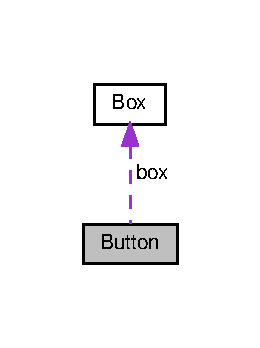
\includegraphics[width=125pt]{structButton__coll__graph}
\end{center}
\end{figure}
\subsection*{Data Fields}
\begin{DoxyCompactItemize}
\item 
\hyperlink{structBox}{Box} \hyperlink{structButton_a0d6f0cb14ea38ae20db8b479a8fce760}{box}
\item 
char $\ast$ \hyperlink{structButton_a78b139339c3b53eb0082803c3b518dad}{name}
\item 
\hyperlink{button_8h_a01cda3effbb71c7c203e4f9716e8844d}{Button\+\_\+state} \hyperlink{structButton_a375398be8d6c20f90febbd0a803b1aec}{state}
\end{DoxyCompactItemize}


\subsection{Field Documentation}
\mbox{\Hypertarget{structButton_a0d6f0cb14ea38ae20db8b479a8fce760}\label{structButton_a0d6f0cb14ea38ae20db8b479a8fce760}} 
\index{Button@{Button}!box@{box}}
\index{box@{box}!Button@{Button}}
\subsubsection{\texorpdfstring{box}{box}}
{\footnotesize\ttfamily \hyperlink{structBox}{Box} Button\+::box}

\mbox{\Hypertarget{structButton_a78b139339c3b53eb0082803c3b518dad}\label{structButton_a78b139339c3b53eb0082803c3b518dad}} 
\index{Button@{Button}!name@{name}}
\index{name@{name}!Button@{Button}}
\subsubsection{\texorpdfstring{name}{name}}
{\footnotesize\ttfamily char$\ast$ Button\+::name}

\mbox{\Hypertarget{structButton_a375398be8d6c20f90febbd0a803b1aec}\label{structButton_a375398be8d6c20f90febbd0a803b1aec}} 
\index{Button@{Button}!state@{state}}
\index{state@{state}!Button@{Button}}
\subsubsection{\texorpdfstring{state}{state}}
{\footnotesize\ttfamily \hyperlink{button_8h_a01cda3effbb71c7c203e4f9716e8844d}{Button\+\_\+state} Button\+::state}



The documentation for this struct was generated from the following file\+:\begin{DoxyCompactItemize}
\item 
includes/\hyperlink{button_8h}{button.\+h}\end{DoxyCompactItemize}

\hypertarget{structErrorList__FirstLast}{}\section{Error\+List\+\_\+\+First\+Last Struct Reference}
\label{structErrorList__FirstLast}\index{Error\+List\+\_\+\+First\+Last@{Error\+List\+\_\+\+First\+Last}}


{\ttfamily \#include $<$list\+\_\+errors.\+h$>$}



Collaboration diagram for Error\+List\+\_\+\+First\+Last\+:\nopagebreak
\begin{figure}[H]
\begin{center}
\leavevmode
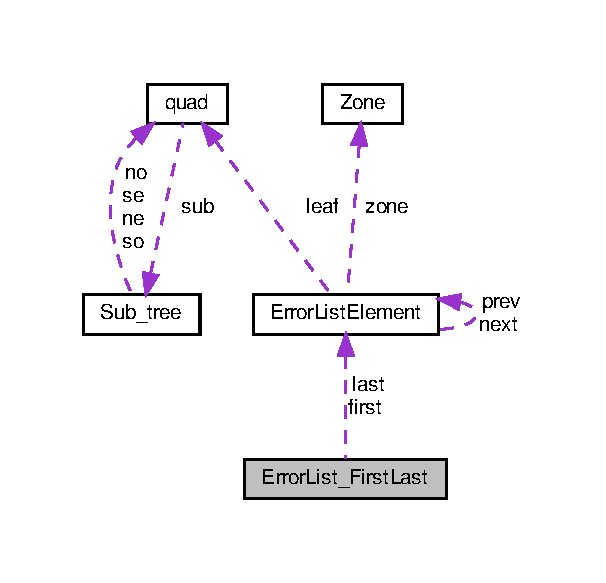
\includegraphics[width=291pt]{structErrorList__FirstLast__coll__graph}
\end{center}
\end{figure}
\subsection*{Data Fields}
\begin{DoxyCompactItemize}
\item 
\hyperlink{list__errors_8h_a90522ae3e839b4beec367e58bc649808}{Error\+List} \hyperlink{structErrorList__FirstLast_a9953e66189d7a875e3c0ce919ae0e243}{first}
\item 
\hyperlink{list__errors_8h_a90522ae3e839b4beec367e58bc649808}{Error\+List} \hyperlink{structErrorList__FirstLast_ab1810567d2d39e9b6784a3b04cde8492}{last}
\end{DoxyCompactItemize}


\subsection{Field Documentation}
\mbox{\Hypertarget{structErrorList__FirstLast_a9953e66189d7a875e3c0ce919ae0e243}\label{structErrorList__FirstLast_a9953e66189d7a875e3c0ce919ae0e243}} 
\index{Error\+List\+\_\+\+First\+Last@{Error\+List\+\_\+\+First\+Last}!first@{first}}
\index{first@{first}!Error\+List\+\_\+\+First\+Last@{Error\+List\+\_\+\+First\+Last}}
\subsubsection{\texorpdfstring{first}{first}}
{\footnotesize\ttfamily \hyperlink{list__errors_8h_a90522ae3e839b4beec367e58bc649808}{Error\+List} Error\+List\+\_\+\+First\+Last\+::first}

\mbox{\Hypertarget{structErrorList__FirstLast_ab1810567d2d39e9b6784a3b04cde8492}\label{structErrorList__FirstLast_ab1810567d2d39e9b6784a3b04cde8492}} 
\index{Error\+List\+\_\+\+First\+Last@{Error\+List\+\_\+\+First\+Last}!last@{last}}
\index{last@{last}!Error\+List\+\_\+\+First\+Last@{Error\+List\+\_\+\+First\+Last}}
\subsubsection{\texorpdfstring{last}{last}}
{\footnotesize\ttfamily \hyperlink{list__errors_8h_a90522ae3e839b4beec367e58bc649808}{Error\+List} Error\+List\+\_\+\+First\+Last\+::last}



The documentation for this struct was generated from the following file\+:\begin{DoxyCompactItemize}
\item 
includes/\hyperlink{list__errors_8h}{list\+\_\+errors.\+h}\end{DoxyCompactItemize}

\hypertarget{structErrorListElement}{}\section{Error\+List\+Element Struct Reference}
\label{structErrorListElement}\index{Error\+List\+Element@{Error\+List\+Element}}


{\ttfamily \#include $<$list\+\_\+errors.\+h$>$}



Collaboration diagram for Error\+List\+Element\+:\nopagebreak
\begin{figure}[H]
\begin{center}
\leavevmode
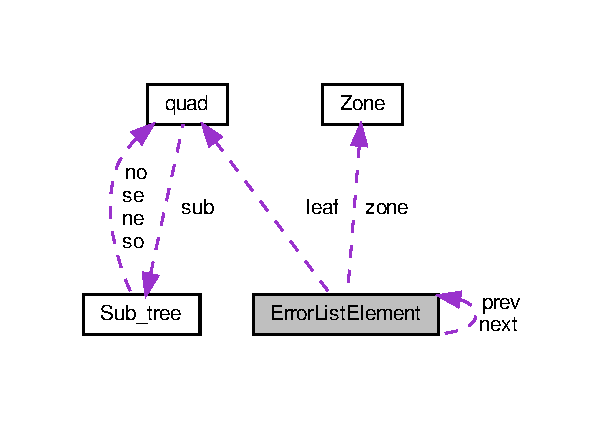
\includegraphics[width=291pt]{structErrorListElement__coll__graph}
\end{center}
\end{figure}
\subsection*{Data Fields}
\begin{DoxyCompactItemize}
\item 
\hyperlink{quadtree_8h_a184f2f10109642ad84b5619bcc5738da}{Tree} $\ast$ \hyperlink{structErrorListElement_aa720e1423b3a1835aac938181639a683}{leaf}
\item 
struct \hyperlink{structErrorListElement}{Error\+List\+Element} $\ast$ \hyperlink{structErrorListElement_a8184726f75bedf47c0b44e71457ed070}{prev}
\item 
struct \hyperlink{structErrorListElement}{Error\+List\+Element} $\ast$ \hyperlink{structErrorListElement_a04526d09e8422e2a18dcea27b81acbc8}{next}
\item 
double \hyperlink{structErrorListElement_ab91e05dff2aa062ae71a3b664f60fc71}{error}
\item 
\hyperlink{structZone}{Zone} \hyperlink{structErrorListElement_a64696b98a5f211dff6ced86e55cf8fe4}{zone}
\end{DoxyCompactItemize}


\subsection{Field Documentation}
\mbox{\Hypertarget{structErrorListElement_ab91e05dff2aa062ae71a3b664f60fc71}\label{structErrorListElement_ab91e05dff2aa062ae71a3b664f60fc71}} 
\index{Error\+List\+Element@{Error\+List\+Element}!error@{error}}
\index{error@{error}!Error\+List\+Element@{Error\+List\+Element}}
\subsubsection{\texorpdfstring{error}{error}}
{\footnotesize\ttfamily double Error\+List\+Element\+::error}

\mbox{\Hypertarget{structErrorListElement_aa720e1423b3a1835aac938181639a683}\label{structErrorListElement_aa720e1423b3a1835aac938181639a683}} 
\index{Error\+List\+Element@{Error\+List\+Element}!leaf@{leaf}}
\index{leaf@{leaf}!Error\+List\+Element@{Error\+List\+Element}}
\subsubsection{\texorpdfstring{leaf}{leaf}}
{\footnotesize\ttfamily \hyperlink{quadtree_8h_a184f2f10109642ad84b5619bcc5738da}{Tree}$\ast$ Error\+List\+Element\+::leaf}

\mbox{\Hypertarget{structErrorListElement_a04526d09e8422e2a18dcea27b81acbc8}\label{structErrorListElement_a04526d09e8422e2a18dcea27b81acbc8}} 
\index{Error\+List\+Element@{Error\+List\+Element}!next@{next}}
\index{next@{next}!Error\+List\+Element@{Error\+List\+Element}}
\subsubsection{\texorpdfstring{next}{next}}
{\footnotesize\ttfamily struct \hyperlink{structErrorListElement}{Error\+List\+Element}$\ast$ Error\+List\+Element\+::next}

\mbox{\Hypertarget{structErrorListElement_a8184726f75bedf47c0b44e71457ed070}\label{structErrorListElement_a8184726f75bedf47c0b44e71457ed070}} 
\index{Error\+List\+Element@{Error\+List\+Element}!prev@{prev}}
\index{prev@{prev}!Error\+List\+Element@{Error\+List\+Element}}
\subsubsection{\texorpdfstring{prev}{prev}}
{\footnotesize\ttfamily struct \hyperlink{structErrorListElement}{Error\+List\+Element}$\ast$ Error\+List\+Element\+::prev}

\mbox{\Hypertarget{structErrorListElement_a64696b98a5f211dff6ced86e55cf8fe4}\label{structErrorListElement_a64696b98a5f211dff6ced86e55cf8fe4}} 
\index{Error\+List\+Element@{Error\+List\+Element}!zone@{zone}}
\index{zone@{zone}!Error\+List\+Element@{Error\+List\+Element}}
\subsubsection{\texorpdfstring{zone}{zone}}
{\footnotesize\ttfamily \hyperlink{structZone}{Zone} Error\+List\+Element\+::zone}



The documentation for this struct was generated from the following file\+:\begin{DoxyCompactItemize}
\item 
includes/\hyperlink{list__errors_8h}{list\+\_\+errors.\+h}\end{DoxyCompactItemize}

\hypertarget{structLeaf__nums}{}\section{Leaf\+\_\+nums Struct Reference}
\label{structLeaf__nums}\index{Leaf\+\_\+nums@{Leaf\+\_\+nums}}


{\ttfamily \#include $<$encoding\+\_\+graph.\+h$>$}

\subsection*{Data Fields}
\begin{DoxyCompactItemize}
\item 
int \hyperlink{structLeaf__nums_a9ed5674a50ffc00ce39d92100ae7ef56}{no}
\item 
int \hyperlink{structLeaf__nums_ae3e6a701d1453d174452c61177ed4852}{ne}
\item 
int \hyperlink{structLeaf__nums_af79e494cdc8b28c367d9ea5b424ddee2}{se}
\item 
int \hyperlink{structLeaf__nums_a32b3e25b99383c612970591174f75885}{so}
\end{DoxyCompactItemize}


\subsection{Field Documentation}
\mbox{\Hypertarget{structLeaf__nums_ae3e6a701d1453d174452c61177ed4852}\label{structLeaf__nums_ae3e6a701d1453d174452c61177ed4852}} 
\index{Leaf\+\_\+nums@{Leaf\+\_\+nums}!ne@{ne}}
\index{ne@{ne}!Leaf\+\_\+nums@{Leaf\+\_\+nums}}
\subsubsection{\texorpdfstring{ne}{ne}}
{\footnotesize\ttfamily int Leaf\+\_\+nums\+::ne}

\mbox{\Hypertarget{structLeaf__nums_a9ed5674a50ffc00ce39d92100ae7ef56}\label{structLeaf__nums_a9ed5674a50ffc00ce39d92100ae7ef56}} 
\index{Leaf\+\_\+nums@{Leaf\+\_\+nums}!no@{no}}
\index{no@{no}!Leaf\+\_\+nums@{Leaf\+\_\+nums}}
\subsubsection{\texorpdfstring{no}{no}}
{\footnotesize\ttfamily int Leaf\+\_\+nums\+::no}

\mbox{\Hypertarget{structLeaf__nums_af79e494cdc8b28c367d9ea5b424ddee2}\label{structLeaf__nums_af79e494cdc8b28c367d9ea5b424ddee2}} 
\index{Leaf\+\_\+nums@{Leaf\+\_\+nums}!se@{se}}
\index{se@{se}!Leaf\+\_\+nums@{Leaf\+\_\+nums}}
\subsubsection{\texorpdfstring{se}{se}}
{\footnotesize\ttfamily int Leaf\+\_\+nums\+::se}

\mbox{\Hypertarget{structLeaf__nums_a32b3e25b99383c612970591174f75885}\label{structLeaf__nums_a32b3e25b99383c612970591174f75885}} 
\index{Leaf\+\_\+nums@{Leaf\+\_\+nums}!so@{so}}
\index{so@{so}!Leaf\+\_\+nums@{Leaf\+\_\+nums}}
\subsubsection{\texorpdfstring{so}{so}}
{\footnotesize\ttfamily int Leaf\+\_\+nums\+::so}



The documentation for this struct was generated from the following file\+:\begin{DoxyCompactItemize}
\item 
includes/\hyperlink{encoding__graph_8h}{encoding\+\_\+graph.\+h}\end{DoxyCompactItemize}

\hypertarget{structMouse}{}\section{Mouse Struct Reference}
\label{structMouse}\index{Mouse@{Mouse}}


{\ttfamily \#include $<$button.\+h$>$}

\subsection*{Data Fields}
\begin{DoxyCompactItemize}
\item 
int \hyperlink{structMouse_a136eea114b70f46392b89cc3779d4291}{x}
\item 
int \hyperlink{structMouse_a4a29b1c18faaa2fbe39ff985ba9d6737}{y}
\item 
M\+L\+V\+\_\+\+Mouse\+\_\+button \hyperlink{structMouse_a326c4f9190419c2aadac8b82c808e11f}{button}
\item 
M\+L\+V\+\_\+\+Button\+\_\+state \hyperlink{structMouse_a4e1a227cd9414b65219cbc7b42e7395d}{state}
\end{DoxyCompactItemize}


\subsection{Field Documentation}
\mbox{\Hypertarget{structMouse_a326c4f9190419c2aadac8b82c808e11f}\label{structMouse_a326c4f9190419c2aadac8b82c808e11f}} 
\index{Mouse@{Mouse}!button@{button}}
\index{button@{button}!Mouse@{Mouse}}
\subsubsection{\texorpdfstring{button}{button}}
{\footnotesize\ttfamily M\+L\+V\+\_\+\+Mouse\+\_\+button Mouse\+::button}

\mbox{\Hypertarget{structMouse_a4e1a227cd9414b65219cbc7b42e7395d}\label{structMouse_a4e1a227cd9414b65219cbc7b42e7395d}} 
\index{Mouse@{Mouse}!state@{state}}
\index{state@{state}!Mouse@{Mouse}}
\subsubsection{\texorpdfstring{state}{state}}
{\footnotesize\ttfamily M\+L\+V\+\_\+\+Button\+\_\+state Mouse\+::state}

\mbox{\Hypertarget{structMouse_a136eea114b70f46392b89cc3779d4291}\label{structMouse_a136eea114b70f46392b89cc3779d4291}} 
\index{Mouse@{Mouse}!x@{x}}
\index{x@{x}!Mouse@{Mouse}}
\subsubsection{\texorpdfstring{x}{x}}
{\footnotesize\ttfamily int Mouse\+::x}

\mbox{\Hypertarget{structMouse_a4a29b1c18faaa2fbe39ff985ba9d6737}\label{structMouse_a4a29b1c18faaa2fbe39ff985ba9d6737}} 
\index{Mouse@{Mouse}!y@{y}}
\index{y@{y}!Mouse@{Mouse}}
\subsubsection{\texorpdfstring{y}{y}}
{\footnotesize\ttfamily int Mouse\+::y}



The documentation for this struct was generated from the following file\+:\begin{DoxyCompactItemize}
\item 
includes/\hyperlink{button_8h}{button.\+h}\end{DoxyCompactItemize}

\hypertarget{structPixel}{}\section{Pixel Struct Reference}
\label{structPixel}\index{Pixel@{Pixel}}


{\ttfamily \#include $<$pixel.\+h$>$}

\subsection*{Data Fields}
\begin{DoxyCompactItemize}
\item 
int \hyperlink{structPixel_a8bdcc8f589c30333ec3f88d2c26d4e3a}{r}
\item 
int \hyperlink{structPixel_a73515f179e3c1bd28156e434da111d05}{g}
\item 
int \hyperlink{structPixel_a94b067f3c79425c953631f7bf1c7536c}{b}
\item 
int \hyperlink{structPixel_aeaad5ecfb916aef136cc8919d8e63a3c}{a}
\end{DoxyCompactItemize}


\subsection{Field Documentation}
\mbox{\Hypertarget{structPixel_aeaad5ecfb916aef136cc8919d8e63a3c}\label{structPixel_aeaad5ecfb916aef136cc8919d8e63a3c}} 
\index{Pixel@{Pixel}!a@{a}}
\index{a@{a}!Pixel@{Pixel}}
\subsubsection{\texorpdfstring{a}{a}}
{\footnotesize\ttfamily int Pixel\+::a}

\mbox{\Hypertarget{structPixel_a94b067f3c79425c953631f7bf1c7536c}\label{structPixel_a94b067f3c79425c953631f7bf1c7536c}} 
\index{Pixel@{Pixel}!b@{b}}
\index{b@{b}!Pixel@{Pixel}}
\subsubsection{\texorpdfstring{b}{b}}
{\footnotesize\ttfamily int Pixel\+::b}

\mbox{\Hypertarget{structPixel_a73515f179e3c1bd28156e434da111d05}\label{structPixel_a73515f179e3c1bd28156e434da111d05}} 
\index{Pixel@{Pixel}!g@{g}}
\index{g@{g}!Pixel@{Pixel}}
\subsubsection{\texorpdfstring{g}{g}}
{\footnotesize\ttfamily int Pixel\+::g}

\mbox{\Hypertarget{structPixel_a8bdcc8f589c30333ec3f88d2c26d4e3a}\label{structPixel_a8bdcc8f589c30333ec3f88d2c26d4e3a}} 
\index{Pixel@{Pixel}!r@{r}}
\index{r@{r}!Pixel@{Pixel}}
\subsubsection{\texorpdfstring{r}{r}}
{\footnotesize\ttfamily int Pixel\+::r}



The documentation for this struct was generated from the following file\+:\begin{DoxyCompactItemize}
\item 
includes/\hyperlink{pixel_8h}{pixel.\+h}\end{DoxyCompactItemize}

\hypertarget{structquad}{}\section{quad Struct Reference}
\label{structquad}\index{quad@{quad}}


{\ttfamily \#include $<$quadtree.\+h$>$}



Collaboration diagram for quad\+:\nopagebreak
\begin{figure}[H]
\begin{center}
\leavevmode
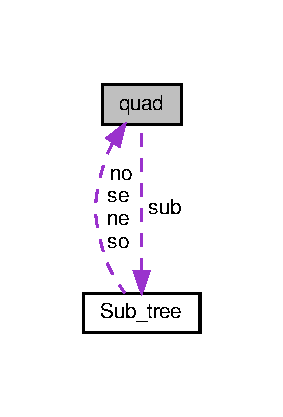
\includegraphics[width=136pt]{structquad__coll__graph}
\end{center}
\end{figure}
\subsection*{Data Fields}
\begin{DoxyCompactItemize}
\item 
\hyperlink{quadtree_8h_a4bafb4a83e1da39fd7547ca43cff608d}{Node\+\_\+type} \hyperlink{structquad_a4c74e17073371714f09bfd5777ce1cc9}{type}
\item 
\hyperlink{unionSub__tree}{Sub\+\_\+tree} $\ast$ \hyperlink{structquad_ac804ea0472312bf6c9191cf863e07ad3}{sub}
\item 
double \hyperlink{structquad_a0431b95089e823b3615f557fe0d9e1eb}{color\+\_\+error}
\end{DoxyCompactItemize}


\subsection{Field Documentation}
\mbox{\Hypertarget{structquad_a0431b95089e823b3615f557fe0d9e1eb}\label{structquad_a0431b95089e823b3615f557fe0d9e1eb}} 
\index{quad@{quad}!color\+\_\+error@{color\+\_\+error}}
\index{color\+\_\+error@{color\+\_\+error}!quad@{quad}}
\subsubsection{\texorpdfstring{color\+\_\+error}{color\_error}}
{\footnotesize\ttfamily double quad\+::color\+\_\+error}

\mbox{\Hypertarget{structquad_ac804ea0472312bf6c9191cf863e07ad3}\label{structquad_ac804ea0472312bf6c9191cf863e07ad3}} 
\index{quad@{quad}!sub@{sub}}
\index{sub@{sub}!quad@{quad}}
\subsubsection{\texorpdfstring{sub}{sub}}
{\footnotesize\ttfamily \hyperlink{unionSub__tree}{Sub\+\_\+tree}$\ast$ quad\+::sub}

\mbox{\Hypertarget{structquad_a4c74e17073371714f09bfd5777ce1cc9}\label{structquad_a4c74e17073371714f09bfd5777ce1cc9}} 
\index{quad@{quad}!type@{type}}
\index{type@{type}!quad@{quad}}
\subsubsection{\texorpdfstring{type}{type}}
{\footnotesize\ttfamily \hyperlink{quadtree_8h_a4bafb4a83e1da39fd7547ca43cff608d}{Node\+\_\+type} quad\+::type}



The documentation for this struct was generated from the following file\+:\begin{DoxyCompactItemize}
\item 
includes/\hyperlink{quadtree_8h}{quadtree.\+h}\end{DoxyCompactItemize}

\hypertarget{unionSub__tree}{}\section{Sub\+\_\+tree Union Reference}
\label{unionSub__tree}\index{Sub\+\_\+tree@{Sub\+\_\+tree}}


{\ttfamily \#include $<$quadtree.\+h$>$}



Collaboration diagram for Sub\+\_\+tree\+:\nopagebreak
\begin{figure}[H]
\begin{center}
\leavevmode
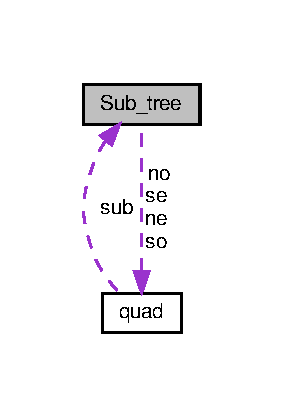
\includegraphics[width=136pt]{unionSub__tree__coll__graph}
\end{center}
\end{figure}
\subsection*{Data Fields}
\begin{DoxyCompactItemize}
\item 
\begin{tabbing}
xx\=xx\=xx\=xx\=xx\=xx\=xx\=xx\=xx\=\kill
struct \{\\
\>struct \hyperlink{structquad}{quad} $\ast$ \hyperlink{unionSub__tree_a28ad496c9c80b56a820758dc35faf753}{no}\\
\>struct \hyperlink{structquad}{quad} $\ast$ \hyperlink{unionSub__tree_a8004244a3434aad839e127a7355d6c6a}{ne}\\
\>struct \hyperlink{structquad}{quad} $\ast$ \hyperlink{unionSub__tree_a85d306e53fc4bae2f6509e444272125c}{so}\\
\>struct \hyperlink{structquad}{quad} $\ast$ \hyperlink{unionSub__tree_acf5c7fe1df5d826c00a8ddc195841b45}{se}\\
\}; \\

\end{tabbing}\item 
M\+L\+V\+\_\+\+Color \hyperlink{unionSub__tree_a956a910a10f18245339a2dd0887bde98}{color}
\end{DoxyCompactItemize}


\subsection{Field Documentation}
\mbox{\Hypertarget{unionSub__tree_a83d224f357140f214eeba416e9f6bb98}\label{unionSub__tree_a83d224f357140f214eeba416e9f6bb98}} 
\subsubsection{\texorpdfstring{"@1}{@1}}
{\footnotesize\ttfamily struct \{ ... \} }

\mbox{\Hypertarget{unionSub__tree_a956a910a10f18245339a2dd0887bde98}\label{unionSub__tree_a956a910a10f18245339a2dd0887bde98}} 
\index{Sub\+\_\+tree@{Sub\+\_\+tree}!color@{color}}
\index{color@{color}!Sub\+\_\+tree@{Sub\+\_\+tree}}
\subsubsection{\texorpdfstring{color}{color}}
{\footnotesize\ttfamily M\+L\+V\+\_\+\+Color Sub\+\_\+tree\+::color}

\mbox{\Hypertarget{unionSub__tree_a8004244a3434aad839e127a7355d6c6a}\label{unionSub__tree_a8004244a3434aad839e127a7355d6c6a}} 
\index{Sub\+\_\+tree@{Sub\+\_\+tree}!ne@{ne}}
\index{ne@{ne}!Sub\+\_\+tree@{Sub\+\_\+tree}}
\subsubsection{\texorpdfstring{ne}{ne}}
{\footnotesize\ttfamily struct \hyperlink{structquad}{quad}$\ast$ Sub\+\_\+tree\+::ne}

\mbox{\Hypertarget{unionSub__tree_a28ad496c9c80b56a820758dc35faf753}\label{unionSub__tree_a28ad496c9c80b56a820758dc35faf753}} 
\index{Sub\+\_\+tree@{Sub\+\_\+tree}!no@{no}}
\index{no@{no}!Sub\+\_\+tree@{Sub\+\_\+tree}}
\subsubsection{\texorpdfstring{no}{no}}
{\footnotesize\ttfamily struct \hyperlink{structquad}{quad}$\ast$ Sub\+\_\+tree\+::no}

\mbox{\Hypertarget{unionSub__tree_acf5c7fe1df5d826c00a8ddc195841b45}\label{unionSub__tree_acf5c7fe1df5d826c00a8ddc195841b45}} 
\index{Sub\+\_\+tree@{Sub\+\_\+tree}!se@{se}}
\index{se@{se}!Sub\+\_\+tree@{Sub\+\_\+tree}}
\subsubsection{\texorpdfstring{se}{se}}
{\footnotesize\ttfamily struct \hyperlink{structquad}{quad}$\ast$ Sub\+\_\+tree\+::se}

\mbox{\Hypertarget{unionSub__tree_a85d306e53fc4bae2f6509e444272125c}\label{unionSub__tree_a85d306e53fc4bae2f6509e444272125c}} 
\index{Sub\+\_\+tree@{Sub\+\_\+tree}!so@{so}}
\index{so@{so}!Sub\+\_\+tree@{Sub\+\_\+tree}}
\subsubsection{\texorpdfstring{so}{so}}
{\footnotesize\ttfamily struct \hyperlink{structquad}{quad}$\ast$ Sub\+\_\+tree\+::so}



The documentation for this union was generated from the following file\+:\begin{DoxyCompactItemize}
\item 
includes/\hyperlink{quadtree_8h}{quadtree.\+h}\end{DoxyCompactItemize}

\hypertarget{structWin}{}\section{Win Struct Reference}
\label{structWin}\index{Win@{Win}}


{\ttfamily \#include $<$window.\+h$>$}



Collaboration diagram for Win\+:\nopagebreak
\begin{figure}[H]
\begin{center}
\leavevmode
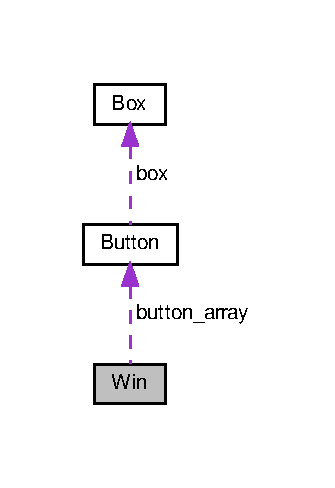
\includegraphics[width=161pt]{structWin__coll__graph}
\end{center}
\end{figure}
\subsection*{Data Fields}
\begin{DoxyCompactItemize}
\item 
int \hyperlink{structWin_a5a16a9f6347e3ce7615537086f1746f0}{nb\+\_\+button}
\item 
int \hyperlink{structWin_a4a7d68b7658b400c0d1f655ed86f2a07}{padding\+\_\+image\+\_\+area}
\item 
int \hyperlink{structWin_a42730d3dc8821c288856ee1dbd3414aa}{padding\+\_\+menu\+\_\+area}
\item 
int \hyperlink{structWin_a6ebae79242d4dff15e5693bbd684ec92}{image\+\_\+tl\+\_\+x}
\item 
int \hyperlink{structWin_a8fe955d73783eb56e0aa7fc4489f3666}{image\+\_\+tl\+\_\+y}
\item 
int \hyperlink{structWin_aa0a54f7537e96b20ed7dd1e162deb5c0}{size\+\_\+x}
\item 
int \hyperlink{structWin_a2cef9065950b7f3f368057ba5372726b}{size\+\_\+y}
\item 
M\+L\+V\+\_\+\+Image $\ast$ \hyperlink{structWin_aca3ad19ffe79c45f6efa4808af338092}{img}
\item 
char $\ast$ \hyperlink{structWin_a17e53cd335af471a25aef8748d89185f}{text\+\_\+input}
\item 
\hyperlink{structButton}{Button} $\ast$ \hyperlink{structWin_ad0f0f707d7f6bad31104bfa1013ee73c}{button\+\_\+array}
\end{DoxyCompactItemize}


\subsection{Field Documentation}
\mbox{\Hypertarget{structWin_ad0f0f707d7f6bad31104bfa1013ee73c}\label{structWin_ad0f0f707d7f6bad31104bfa1013ee73c}} 
\index{Win@{Win}!button\+\_\+array@{button\+\_\+array}}
\index{button\+\_\+array@{button\+\_\+array}!Win@{Win}}
\subsubsection{\texorpdfstring{button\+\_\+array}{button\_array}}
{\footnotesize\ttfamily \hyperlink{structButton}{Button}$\ast$ Win\+::button\+\_\+array}

\mbox{\Hypertarget{structWin_a6ebae79242d4dff15e5693bbd684ec92}\label{structWin_a6ebae79242d4dff15e5693bbd684ec92}} 
\index{Win@{Win}!image\+\_\+tl\+\_\+x@{image\+\_\+tl\+\_\+x}}
\index{image\+\_\+tl\+\_\+x@{image\+\_\+tl\+\_\+x}!Win@{Win}}
\subsubsection{\texorpdfstring{image\+\_\+tl\+\_\+x}{image\_tl\_x}}
{\footnotesize\ttfamily int Win\+::image\+\_\+tl\+\_\+x}

\mbox{\Hypertarget{structWin_a8fe955d73783eb56e0aa7fc4489f3666}\label{structWin_a8fe955d73783eb56e0aa7fc4489f3666}} 
\index{Win@{Win}!image\+\_\+tl\+\_\+y@{image\+\_\+tl\+\_\+y}}
\index{image\+\_\+tl\+\_\+y@{image\+\_\+tl\+\_\+y}!Win@{Win}}
\subsubsection{\texorpdfstring{image\+\_\+tl\+\_\+y}{image\_tl\_y}}
{\footnotesize\ttfamily int Win\+::image\+\_\+tl\+\_\+y}

\mbox{\Hypertarget{structWin_aca3ad19ffe79c45f6efa4808af338092}\label{structWin_aca3ad19ffe79c45f6efa4808af338092}} 
\index{Win@{Win}!img@{img}}
\index{img@{img}!Win@{Win}}
\subsubsection{\texorpdfstring{img}{img}}
{\footnotesize\ttfamily M\+L\+V\+\_\+\+Image$\ast$ Win\+::img}

\mbox{\Hypertarget{structWin_a5a16a9f6347e3ce7615537086f1746f0}\label{structWin_a5a16a9f6347e3ce7615537086f1746f0}} 
\index{Win@{Win}!nb\+\_\+button@{nb\+\_\+button}}
\index{nb\+\_\+button@{nb\+\_\+button}!Win@{Win}}
\subsubsection{\texorpdfstring{nb\+\_\+button}{nb\_button}}
{\footnotesize\ttfamily int Win\+::nb\+\_\+button}

\mbox{\Hypertarget{structWin_a4a7d68b7658b400c0d1f655ed86f2a07}\label{structWin_a4a7d68b7658b400c0d1f655ed86f2a07}} 
\index{Win@{Win}!padding\+\_\+image\+\_\+area@{padding\+\_\+image\+\_\+area}}
\index{padding\+\_\+image\+\_\+area@{padding\+\_\+image\+\_\+area}!Win@{Win}}
\subsubsection{\texorpdfstring{padding\+\_\+image\+\_\+area}{padding\_image\_area}}
{\footnotesize\ttfamily int Win\+::padding\+\_\+image\+\_\+area}

\mbox{\Hypertarget{structWin_a42730d3dc8821c288856ee1dbd3414aa}\label{structWin_a42730d3dc8821c288856ee1dbd3414aa}} 
\index{Win@{Win}!padding\+\_\+menu\+\_\+area@{padding\+\_\+menu\+\_\+area}}
\index{padding\+\_\+menu\+\_\+area@{padding\+\_\+menu\+\_\+area}!Win@{Win}}
\subsubsection{\texorpdfstring{padding\+\_\+menu\+\_\+area}{padding\_menu\_area}}
{\footnotesize\ttfamily int Win\+::padding\+\_\+menu\+\_\+area}

\mbox{\Hypertarget{structWin_aa0a54f7537e96b20ed7dd1e162deb5c0}\label{structWin_aa0a54f7537e96b20ed7dd1e162deb5c0}} 
\index{Win@{Win}!size\+\_\+x@{size\+\_\+x}}
\index{size\+\_\+x@{size\+\_\+x}!Win@{Win}}
\subsubsection{\texorpdfstring{size\+\_\+x}{size\_x}}
{\footnotesize\ttfamily int Win\+::size\+\_\+x}

\mbox{\Hypertarget{structWin_a2cef9065950b7f3f368057ba5372726b}\label{structWin_a2cef9065950b7f3f368057ba5372726b}} 
\index{Win@{Win}!size\+\_\+y@{size\+\_\+y}}
\index{size\+\_\+y@{size\+\_\+y}!Win@{Win}}
\subsubsection{\texorpdfstring{size\+\_\+y}{size\_y}}
{\footnotesize\ttfamily int Win\+::size\+\_\+y}

\mbox{\Hypertarget{structWin_a17e53cd335af471a25aef8748d89185f}\label{structWin_a17e53cd335af471a25aef8748d89185f}} 
\index{Win@{Win}!text\+\_\+input@{text\+\_\+input}}
\index{text\+\_\+input@{text\+\_\+input}!Win@{Win}}
\subsubsection{\texorpdfstring{text\+\_\+input}{text\_input}}
{\footnotesize\ttfamily char$\ast$ Win\+::text\+\_\+input}



The documentation for this struct was generated from the following file\+:\begin{DoxyCompactItemize}
\item 
includes/\hyperlink{window_8h}{window.\+h}\end{DoxyCompactItemize}

\hypertarget{structZone}{}\section{Zone Struct Reference}
\label{structZone}\index{Zone@{Zone}}


{\ttfamily \#include $<$zone.\+h$>$}

\subsection*{Data Fields}
\begin{DoxyCompactItemize}
\item 
int \hyperlink{structZone_af3a495f8656e34f4d2ed8429ada7aed9}{x1}
\item 
int \hyperlink{structZone_ab160ed8f9ec2dc6efef018e743f94683}{y1}
\item 
int \hyperlink{structZone_a6643320a49b430fa1cc69aac133f6da6}{x2}
\item 
int \hyperlink{structZone_a7cf6801d4594d045c56368c35fe8c7e2}{y2}
\end{DoxyCompactItemize}


\subsection{Field Documentation}
\mbox{\Hypertarget{structZone_af3a495f8656e34f4d2ed8429ada7aed9}\label{structZone_af3a495f8656e34f4d2ed8429ada7aed9}} 
\index{Zone@{Zone}!x1@{x1}}
\index{x1@{x1}!Zone@{Zone}}
\subsubsection{\texorpdfstring{x1}{x1}}
{\footnotesize\ttfamily int Zone\+::x1}

\mbox{\Hypertarget{structZone_a6643320a49b430fa1cc69aac133f6da6}\label{structZone_a6643320a49b430fa1cc69aac133f6da6}} 
\index{Zone@{Zone}!x2@{x2}}
\index{x2@{x2}!Zone@{Zone}}
\subsubsection{\texorpdfstring{x2}{x2}}
{\footnotesize\ttfamily int Zone\+::x2}

\mbox{\Hypertarget{structZone_ab160ed8f9ec2dc6efef018e743f94683}\label{structZone_ab160ed8f9ec2dc6efef018e743f94683}} 
\index{Zone@{Zone}!y1@{y1}}
\index{y1@{y1}!Zone@{Zone}}
\subsubsection{\texorpdfstring{y1}{y1}}
{\footnotesize\ttfamily int Zone\+::y1}

\mbox{\Hypertarget{structZone_a7cf6801d4594d045c56368c35fe8c7e2}\label{structZone_a7cf6801d4594d045c56368c35fe8c7e2}} 
\index{Zone@{Zone}!y2@{y2}}
\index{y2@{y2}!Zone@{Zone}}
\subsubsection{\texorpdfstring{y2}{y2}}
{\footnotesize\ttfamily int Zone\+::y2}



The documentation for this struct was generated from the following file\+:\begin{DoxyCompactItemize}
\item 
includes/\hyperlink{zone_8h}{zone.\+h}\end{DoxyCompactItemize}

\chapter{File Documentation}
\hypertarget{bit__buffer_8h}{}\section{includes/bit\+\_\+buffer.h File Reference}
\label{bit__buffer_8h}\index{includes/bit\+\_\+buffer.\+h@{includes/bit\+\_\+buffer.\+h}}
{\ttfamily \#include $<$stdio.\+h$>$}\newline
{\ttfamily \#include $<$stdint.\+h$>$}\newline
Include dependency graph for bit\+\_\+buffer.\+h\+:
\nopagebreak
\begin{figure}[H]
\begin{center}
\leavevmode
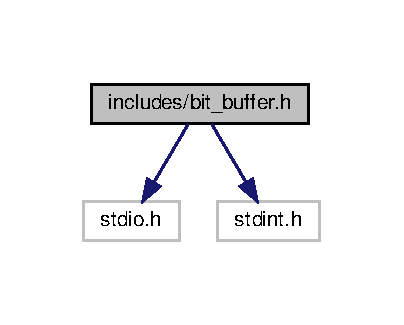
\includegraphics[width=194pt]{bit__buffer_8h__incl}
\end{center}
\end{figure}
This graph shows which files directly or indirectly include this file\+:
\nopagebreak
\begin{figure}[H]
\begin{center}
\leavevmode
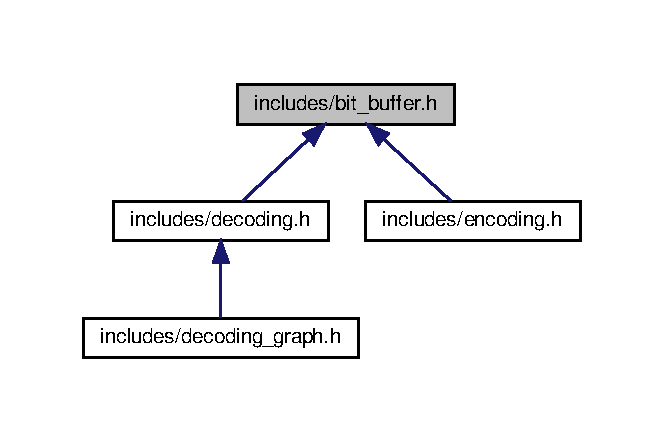
\includegraphics[width=319pt]{bit__buffer_8h__dep__incl}
\end{center}
\end{figure}
\subsection*{Data Structures}
\begin{DoxyCompactItemize}
\item 
struct \hyperlink{structBit__buffer}{Bit\+\_\+buffer}
\end{DoxyCompactItemize}
\subsection*{Functions}
\begin{DoxyCompactItemize}
\item 
void \hyperlink{bit__buffer_8h_aa7dba68df08c09b3e7aa209e01afcc79}{init\+\_\+bit\+\_\+buffer} (\hyperlink{structBit__buffer}{Bit\+\_\+buffer} $\ast$bit\+\_\+buffer)
\begin{DoxyCompactList}\small\item\em Initialize a bit\+\_\+buffer. \end{DoxyCompactList}\item 
void \hyperlink{bit__buffer_8h_acfe8e739139f45be71bf672b64c8e208}{padding\+\_\+last\+\_\+oct} (\hyperlink{structBit__buffer}{Bit\+\_\+buffer} $\ast$bit\+\_\+buffer, F\+I\+LE $\ast$file)
\begin{DoxyCompactList}\small\item\em Add \textquotesingle{}0\textquotesingle{} to bit\+\_\+buffer in order to complete the byte. \end{DoxyCompactList}\item 
void \hyperlink{bit__buffer_8h_acce7d6528363885bf2bf46f6ec3f0e6e}{write\+\_\+bit} (\hyperlink{structBit__buffer}{Bit\+\_\+buffer} $\ast$bit\+\_\+buffer, int val, F\+I\+LE $\ast$file)
\begin{DoxyCompactList}\small\item\em Fill a bit\+\_\+buffer depending of the value of \char`\"{}val\char`\"{} If val != 0, add 1 to bit\+\_\+buffer If val == 0, add 0 to bit\+\_\+buffer. \end{DoxyCompactList}\item 
void \hyperlink{bit__buffer_8h_a1ddbad580747e02386339bd894d725a7}{write\+\_\+bit\+\_\+color} (\hyperlink{structBit__buffer}{Bit\+\_\+buffer} $\ast$bit\+\_\+buffer, unsigned char color, F\+I\+LE $\ast$file)
\begin{DoxyCompactList}\small\item\em Convert color into a byte, and write it in file. \end{DoxyCompactList}\item 
int \hyperlink{bit__buffer_8h_a53ef7e8afa087bcb6769530974f3dada}{read\+\_\+bit} (\hyperlink{structBit__buffer}{Bit\+\_\+buffer} $\ast$bit\+\_\+buffer, F\+I\+LE $\ast$file)
\begin{DoxyCompactList}\small\item\em Read the current bit in bit\+\_\+buffer If we have read all the bit, fgetc in order to get the file next byte. \end{DoxyCompactList}\end{DoxyCompactItemize}


\subsection{Function Documentation}
\mbox{\Hypertarget{bit__buffer_8h_aa7dba68df08c09b3e7aa209e01afcc79}\label{bit__buffer_8h_aa7dba68df08c09b3e7aa209e01afcc79}} 
\index{bit\+\_\+buffer.\+h@{bit\+\_\+buffer.\+h}!init\+\_\+bit\+\_\+buffer@{init\+\_\+bit\+\_\+buffer}}
\index{init\+\_\+bit\+\_\+buffer@{init\+\_\+bit\+\_\+buffer}!bit\+\_\+buffer.\+h@{bit\+\_\+buffer.\+h}}
\subsubsection{\texorpdfstring{init\+\_\+bit\+\_\+buffer()}{init\_bit\_buffer()}}
{\footnotesize\ttfamily void init\+\_\+bit\+\_\+buffer (\begin{DoxyParamCaption}\item[{\hyperlink{structBit__buffer}{Bit\+\_\+buffer} $\ast$}]{bit\+\_\+buffer }\end{DoxyParamCaption})}



Initialize a bit\+\_\+buffer. 


\begin{DoxyParams}{Parameters}
{\em bit\+\_\+buffer} & The bit\+\_\+buffer we are initializing \\
\hline
\end{DoxyParams}
\mbox{\Hypertarget{bit__buffer_8h_acfe8e739139f45be71bf672b64c8e208}\label{bit__buffer_8h_acfe8e739139f45be71bf672b64c8e208}} 
\index{bit\+\_\+buffer.\+h@{bit\+\_\+buffer.\+h}!padding\+\_\+last\+\_\+oct@{padding\+\_\+last\+\_\+oct}}
\index{padding\+\_\+last\+\_\+oct@{padding\+\_\+last\+\_\+oct}!bit\+\_\+buffer.\+h@{bit\+\_\+buffer.\+h}}
\subsubsection{\texorpdfstring{padding\+\_\+last\+\_\+oct()}{padding\_last\_oct()}}
{\footnotesize\ttfamily void padding\+\_\+last\+\_\+oct (\begin{DoxyParamCaption}\item[{\hyperlink{structBit__buffer}{Bit\+\_\+buffer} $\ast$}]{bit\+\_\+buffer,  }\item[{F\+I\+LE $\ast$}]{file }\end{DoxyParamCaption})}



Add \textquotesingle{}0\textquotesingle{} to bit\+\_\+buffer in order to complete the byte. 


\begin{DoxyParams}{Parameters}
{\em bit\+\_\+buffer} & The bit\+\_\+buffer we are \char`\"{}padding\char`\"{} \\
\hline
{\em file} & The file we are writing in \\
\hline
\end{DoxyParams}
\mbox{\Hypertarget{bit__buffer_8h_a53ef7e8afa087bcb6769530974f3dada}\label{bit__buffer_8h_a53ef7e8afa087bcb6769530974f3dada}} 
\index{bit\+\_\+buffer.\+h@{bit\+\_\+buffer.\+h}!read\+\_\+bit@{read\+\_\+bit}}
\index{read\+\_\+bit@{read\+\_\+bit}!bit\+\_\+buffer.\+h@{bit\+\_\+buffer.\+h}}
\subsubsection{\texorpdfstring{read\+\_\+bit()}{read\_bit()}}
{\footnotesize\ttfamily int read\+\_\+bit (\begin{DoxyParamCaption}\item[{\hyperlink{structBit__buffer}{Bit\+\_\+buffer} $\ast$}]{bit\+\_\+buffer,  }\item[{F\+I\+LE $\ast$}]{file }\end{DoxyParamCaption})}



Read the current bit in bit\+\_\+buffer If we have read all the bit, fgetc in order to get the file next byte. 


\begin{DoxyParams}{Parameters}
{\em bit\+\_\+buffer} & The bit\+\_\+buffer we get the byte from, and read from \\
\hline
{\em file} & The file we are reading \\
\hline
\end{DoxyParams}
\begin{DoxyReturn}{Returns}
Current value of bit\+\_\+buffer (0 or 1) 
\end{DoxyReturn}
\mbox{\Hypertarget{bit__buffer_8h_acce7d6528363885bf2bf46f6ec3f0e6e}\label{bit__buffer_8h_acce7d6528363885bf2bf46f6ec3f0e6e}} 
\index{bit\+\_\+buffer.\+h@{bit\+\_\+buffer.\+h}!write\+\_\+bit@{write\+\_\+bit}}
\index{write\+\_\+bit@{write\+\_\+bit}!bit\+\_\+buffer.\+h@{bit\+\_\+buffer.\+h}}
\subsubsection{\texorpdfstring{write\+\_\+bit()}{write\_bit()}}
{\footnotesize\ttfamily void write\+\_\+bit (\begin{DoxyParamCaption}\item[{\hyperlink{structBit__buffer}{Bit\+\_\+buffer} $\ast$}]{bit\+\_\+buffer,  }\item[{int}]{val,  }\item[{F\+I\+LE $\ast$}]{file }\end{DoxyParamCaption})}



Fill a bit\+\_\+buffer depending of the value of \char`\"{}val\char`\"{} If val != 0, add 1 to bit\+\_\+buffer If val == 0, add 0 to bit\+\_\+buffer. 


\begin{DoxyParams}{Parameters}
{\em bit\+\_\+buffer} & The bit\+\_\+buffer we are filling \\
\hline
{\em val} & The value \\
\hline
{\em file} & The file we are writing in if bit\+\_\+buffer is full (byte completed) \\
\hline
\end{DoxyParams}
\mbox{\Hypertarget{bit__buffer_8h_a1ddbad580747e02386339bd894d725a7}\label{bit__buffer_8h_a1ddbad580747e02386339bd894d725a7}} 
\index{bit\+\_\+buffer.\+h@{bit\+\_\+buffer.\+h}!write\+\_\+bit\+\_\+color@{write\+\_\+bit\+\_\+color}}
\index{write\+\_\+bit\+\_\+color@{write\+\_\+bit\+\_\+color}!bit\+\_\+buffer.\+h@{bit\+\_\+buffer.\+h}}
\subsubsection{\texorpdfstring{write\+\_\+bit\+\_\+color()}{write\_bit\_color()}}
{\footnotesize\ttfamily void write\+\_\+bit\+\_\+color (\begin{DoxyParamCaption}\item[{\hyperlink{structBit__buffer}{Bit\+\_\+buffer} $\ast$}]{bit\+\_\+buffer,  }\item[{unsigned char}]{color,  }\item[{F\+I\+LE $\ast$}]{file }\end{DoxyParamCaption})}



Convert color into a byte, and write it in file. 


\begin{DoxyParams}{Parameters}
{\em bit\+\_\+buffer} & The bit\+\_\+buffer we are filling in order to write color in the file \\
\hline
{\em color} & The color we want to add in file \\
\hline
{\em file} & The file we are writing the color in \\
\hline
\end{DoxyParams}

\hypertarget{button_8h}{}\section{includes/button.h File Reference}
\label{button_8h}\index{includes/button.\+h@{includes/button.\+h}}
{\ttfamily \#include $<$M\+L\+V/\+M\+L\+V\+\_\+all.\+h$>$}\newline
Include dependency graph for button.\+h\+:
\nopagebreak
\begin{figure}[H]
\begin{center}
\leavevmode
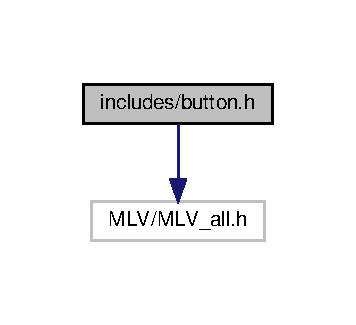
\includegraphics[width=171pt]{button_8h__incl}
\end{center}
\end{figure}
This graph shows which files directly or indirectly include this file\+:
\nopagebreak
\begin{figure}[H]
\begin{center}
\leavevmode
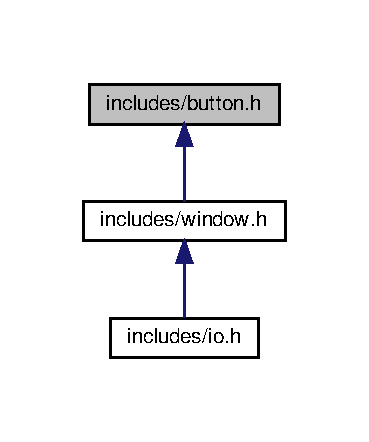
\includegraphics[width=177pt]{button_8h__dep__incl}
\end{center}
\end{figure}
\subsection*{Data Structures}
\begin{DoxyCompactItemize}
\item 
struct \hyperlink{structMouse}{Mouse}
\item 
struct \hyperlink{structBox}{Box}
\item 
struct \hyperlink{structButton}{Button}
\end{DoxyCompactItemize}
\subsection*{Macros}
\begin{DoxyCompactItemize}
\item 
\#define \hyperlink{button_8h_aa6a14d1d8be58caed6952171e0b4c706}{B\+T\+N\+\_\+\+B\+G\+\_\+\+H\+O\+V\+ER}~M\+L\+V\+\_\+\+C\+O\+L\+O\+R\+\_\+\+L\+I\+G\+H\+T\+\_\+\+S\+E\+A\+\_\+\+G\+R\+E\+EN
\item 
\#define \hyperlink{button_8h_a7021af036c5ab0d51c9cae138016e95f}{B\+T\+N\+\_\+\+B\+G\+\_\+\+H\+E\+LD}~M\+L\+V\+\_\+\+C\+O\+L\+O\+R\+\_\+\+P\+A\+L\+E\+\_\+\+G\+R\+E\+EN
\item 
\#define \hyperlink{button_8h_aed0fae86ebe3ab29e6846dc0ab25c32b}{B\+T\+N\+\_\+\+B\+G\+\_\+\+B\+U\+I\+SY}~M\+L\+V\+\_\+\+C\+O\+L\+O\+R\+\_\+\+T\+AN
\item 
\#define \hyperlink{button_8h_a552c77610827a82c70b55b1d0bdd5ba4}{B\+T\+N\+\_\+\+B\+G\+\_\+\+A\+V\+A\+I\+L\+A\+B\+LE}~M\+L\+V\+\_\+\+C\+O\+L\+O\+R\+\_\+\+G\+R\+E\+EN
\item 
\#define \hyperlink{button_8h_a970f18109a00139e94cf28f9f0f65223}{B\+T\+N\+\_\+\+B\+G\+\_\+\+F\+O\+R\+B\+I\+D\+EN}~M\+L\+V\+\_\+\+C\+O\+L\+O\+R\+\_\+\+G\+R\+EY
\item 
\#define \hyperlink{button_8h_ad9700fecd671cd74fdb9c7540a00a214}{B\+T\+N\+\_\+\+B\+O\+D\+E\+R\+\_\+\+H\+O\+V\+ER}~M\+L\+V\+\_\+\+C\+O\+L\+O\+R\+\_\+\+Y\+E\+L\+L\+OW
\item 
\#define \hyperlink{button_8h_ae130ca39d1a354904dc570eb77d4add0}{B\+T\+N\+\_\+\+B\+O\+D\+E\+R\+\_\+\+H\+E\+LD}~M\+L\+V\+\_\+\+C\+O\+L\+O\+R\+\_\+\+L\+I\+G\+H\+T\+\_\+\+G\+O\+L\+D\+E\+N\+R\+OD
\item 
\#define \hyperlink{button_8h_ab7612caea312bea76733365d5b915bcf}{B\+T\+N\+\_\+\+B\+O\+D\+E\+R\+\_\+\+B\+U\+I\+SY}~M\+L\+V\+\_\+\+C\+O\+L\+O\+R\+\_\+\+D\+A\+R\+K\+\_\+\+G\+O\+L\+D\+E\+N\+R\+OD
\item 
\#define \hyperlink{button_8h_aab30d3dae8b07eaa0de563639180b906}{B\+T\+N\+\_\+\+B\+O\+D\+E\+R\+\_\+\+A\+V\+A\+I\+L\+A\+B\+LE}~M\+L\+V\+\_\+\+C\+O\+L\+O\+R\+\_\+\+G\+O\+LD
\item 
\#define \hyperlink{button_8h_a32bbb00b42053e789e5934187f6dae88}{B\+T\+N\+\_\+\+B\+O\+D\+E\+R\+\_\+\+F\+O\+R\+B\+I\+D\+EN}~M\+L\+V\+\_\+\+C\+O\+L\+O\+R\+\_\+\+A\+N\+T\+I\+Q\+U\+E\+\_\+\+W\+H\+I\+TE
\item 
\#define \hyperlink{button_8h_a085714deb8b077fe2ecacfa7da3ff919}{B\+T\+N\+\_\+\+T\+E\+X\+T\+\_\+\+H\+O\+V\+ER}~M\+L\+V\+\_\+\+C\+O\+L\+O\+R\+\_\+\+A\+N\+T\+I\+Q\+U\+E\+\_\+\+W\+H\+I\+TE
\item 
\#define \hyperlink{button_8h_a32dc1301e17c95894ace0575f20994d5}{B\+T\+N\+\_\+\+T\+E\+X\+T\+\_\+\+H\+E\+LD}~M\+L\+V\+\_\+\+C\+O\+L\+O\+R\+\_\+\+B\+L\+A\+CK
\item 
\#define \hyperlink{button_8h_a380329c65e2a7a5e7e255aba8ca940b3}{B\+T\+N\+\_\+\+T\+E\+X\+T\+\_\+\+B\+U\+I\+SY}~M\+L\+V\+\_\+\+C\+O\+L\+O\+R\+\_\+\+G\+A\+I\+N\+S\+B\+O\+RO
\item 
\#define \hyperlink{button_8h_a679162ca7bca2ba1b2cfa411683ff06e}{B\+T\+N\+\_\+\+T\+E\+X\+T\+\_\+\+A\+V\+A\+I\+L\+A\+B\+LE}~M\+L\+V\+\_\+\+C\+O\+L\+O\+R\+\_\+\+B\+L\+A\+CK
\item 
\#define \hyperlink{button_8h_a2ed753768a60cd6fd9b30800e76a1de7}{B\+T\+N\+\_\+\+T\+E\+X\+T\+\_\+\+F\+O\+R\+B\+I\+D\+EN}~M\+L\+V\+\_\+\+C\+O\+L\+O\+R\+\_\+\+B\+L\+A\+CK
\item 
\#define \hyperlink{button_8h_aac775283f3d16d035ad1753409e2a632}{B\+T\+N\+\_\+\+H\+E\+I\+G\+HT}~48
\item 
\#define \hyperlink{button_8h_ae4103c363ed830afddd072ef363726da}{B\+T\+N\+\_\+\+W\+I\+D\+TH}~175
\end{DoxyCompactItemize}
\subsection*{Enumerations}
\begin{DoxyCompactItemize}
\item 
enum \hyperlink{button_8h_a01cda3effbb71c7c203e4f9716e8844d}{Button\+\_\+state} \{ \newline
\hyperlink{button_8h_a01cda3effbb71c7c203e4f9716e8844da13da5684f960f9c5979c7b4d8da465dd}{B\+U\+I\+SY}, 
\hyperlink{button_8h_a01cda3effbb71c7c203e4f9716e8844dac0d64bfdd0f176c021eac3fca2be30af}{H\+E\+LD}, 
\hyperlink{button_8h_a01cda3effbb71c7c203e4f9716e8844da1e229ccb8b53a57de4ebb11c2d15272e}{A\+V\+A\+I\+L\+A\+B\+LE}, 
\hyperlink{button_8h_a01cda3effbb71c7c203e4f9716e8844da8df21af5ed7da4b83ff86f107b52ef75}{H\+O\+V\+ER}, 
\newline
\hyperlink{button_8h_a01cda3effbb71c7c203e4f9716e8844dae099fdefa5afa14f6b23f596c972ce16}{F\+O\+R\+B\+I\+D\+EN}
 \}
\end{DoxyCompactItemize}
\subsection*{Functions}
\begin{DoxyCompactItemize}
\item 
int \hyperlink{button_8h_acd0e5c2dc8b53fbad47ce6027726c940}{add\+\_\+button} (int tl\+\_\+x, int tl\+\_\+y, int height, int width, const char $\ast$name, int $\ast$nb\+\_\+button, \hyperlink{structButton}{Button} $\ast$$\ast$array)
\begin{DoxyCompactList}\small\item\em This function adds a button to the window. \end{DoxyCompactList}\item 
void \hyperlink{button_8h_a70e1acd3fe18f11cee78040d92fa9879}{free\+\_\+button\+\_\+array} (int nb\+\_\+button, \hyperlink{structButton}{Button} $\ast$$\ast$array)
\begin{DoxyCompactList}\small\item\em This function frees the buttons allocated by \textquotesingle{}add\+\_\+button\textquotesingle{}. \end{DoxyCompactList}\item 
void \hyperlink{button_8h_a3c80ef62c406b246a116261e1b1b33b2}{display\+\_\+all\+\_\+button} (int nb\+\_\+button, \hyperlink{structButton}{Button} $\ast$array)
\begin{DoxyCompactList}\small\item\em This function displays the buttons according to their \textquotesingle{}state\textquotesingle{} field. \end{DoxyCompactList}\item 
void \hyperlink{button_8h_a2600cefe39d33af6da45dd6ec3730c12}{print\+\_\+all\+\_\+button} (int nb\+\_\+button, \hyperlink{structButton}{Button} $\ast$array)
\begin{DoxyCompactList}\small\item\em This function print all button in the array in the console. \end{DoxyCompactList}\item 
int \hyperlink{button_8h_a08fe0799d78bc25281b9cfd66efe0f4e}{button\+\_\+update} (\hyperlink{structMouse}{Mouse} $\ast$mouse, \hyperlink{structButton}{Button} $\ast$array, int nb\+\_\+button, const M\+L\+V\+\_\+\+Event ev)
\begin{DoxyCompactList}\small\item\em This function updates the state of the button acording to the mouse events. \end{DoxyCompactList}\end{DoxyCompactItemize}


\subsection{Macro Definition Documentation}
\mbox{\Hypertarget{button_8h_a552c77610827a82c70b55b1d0bdd5ba4}\label{button_8h_a552c77610827a82c70b55b1d0bdd5ba4}} 
\index{button.\+h@{button.\+h}!B\+T\+N\+\_\+\+B\+G\+\_\+\+A\+V\+A\+I\+L\+A\+B\+LE@{B\+T\+N\+\_\+\+B\+G\+\_\+\+A\+V\+A\+I\+L\+A\+B\+LE}}
\index{B\+T\+N\+\_\+\+B\+G\+\_\+\+A\+V\+A\+I\+L\+A\+B\+LE@{B\+T\+N\+\_\+\+B\+G\+\_\+\+A\+V\+A\+I\+L\+A\+B\+LE}!button.\+h@{button.\+h}}
\subsubsection{\texorpdfstring{B\+T\+N\+\_\+\+B\+G\+\_\+\+A\+V\+A\+I\+L\+A\+B\+LE}{BTN\_BG\_AVAILABLE}}
{\footnotesize\ttfamily \#define B\+T\+N\+\_\+\+B\+G\+\_\+\+A\+V\+A\+I\+L\+A\+B\+LE~M\+L\+V\+\_\+\+C\+O\+L\+O\+R\+\_\+\+G\+R\+E\+EN}

\mbox{\Hypertarget{button_8h_aed0fae86ebe3ab29e6846dc0ab25c32b}\label{button_8h_aed0fae86ebe3ab29e6846dc0ab25c32b}} 
\index{button.\+h@{button.\+h}!B\+T\+N\+\_\+\+B\+G\+\_\+\+B\+U\+I\+SY@{B\+T\+N\+\_\+\+B\+G\+\_\+\+B\+U\+I\+SY}}
\index{B\+T\+N\+\_\+\+B\+G\+\_\+\+B\+U\+I\+SY@{B\+T\+N\+\_\+\+B\+G\+\_\+\+B\+U\+I\+SY}!button.\+h@{button.\+h}}
\subsubsection{\texorpdfstring{B\+T\+N\+\_\+\+B\+G\+\_\+\+B\+U\+I\+SY}{BTN\_BG\_BUISY}}
{\footnotesize\ttfamily \#define B\+T\+N\+\_\+\+B\+G\+\_\+\+B\+U\+I\+SY~M\+L\+V\+\_\+\+C\+O\+L\+O\+R\+\_\+\+T\+AN}

\mbox{\Hypertarget{button_8h_a970f18109a00139e94cf28f9f0f65223}\label{button_8h_a970f18109a00139e94cf28f9f0f65223}} 
\index{button.\+h@{button.\+h}!B\+T\+N\+\_\+\+B\+G\+\_\+\+F\+O\+R\+B\+I\+D\+EN@{B\+T\+N\+\_\+\+B\+G\+\_\+\+F\+O\+R\+B\+I\+D\+EN}}
\index{B\+T\+N\+\_\+\+B\+G\+\_\+\+F\+O\+R\+B\+I\+D\+EN@{B\+T\+N\+\_\+\+B\+G\+\_\+\+F\+O\+R\+B\+I\+D\+EN}!button.\+h@{button.\+h}}
\subsubsection{\texorpdfstring{B\+T\+N\+\_\+\+B\+G\+\_\+\+F\+O\+R\+B\+I\+D\+EN}{BTN\_BG\_FORBIDEN}}
{\footnotesize\ttfamily \#define B\+T\+N\+\_\+\+B\+G\+\_\+\+F\+O\+R\+B\+I\+D\+EN~M\+L\+V\+\_\+\+C\+O\+L\+O\+R\+\_\+\+G\+R\+EY}

\mbox{\Hypertarget{button_8h_a7021af036c5ab0d51c9cae138016e95f}\label{button_8h_a7021af036c5ab0d51c9cae138016e95f}} 
\index{button.\+h@{button.\+h}!B\+T\+N\+\_\+\+B\+G\+\_\+\+H\+E\+LD@{B\+T\+N\+\_\+\+B\+G\+\_\+\+H\+E\+LD}}
\index{B\+T\+N\+\_\+\+B\+G\+\_\+\+H\+E\+LD@{B\+T\+N\+\_\+\+B\+G\+\_\+\+H\+E\+LD}!button.\+h@{button.\+h}}
\subsubsection{\texorpdfstring{B\+T\+N\+\_\+\+B\+G\+\_\+\+H\+E\+LD}{BTN\_BG\_HELD}}
{\footnotesize\ttfamily \#define B\+T\+N\+\_\+\+B\+G\+\_\+\+H\+E\+LD~M\+L\+V\+\_\+\+C\+O\+L\+O\+R\+\_\+\+P\+A\+L\+E\+\_\+\+G\+R\+E\+EN}

\mbox{\Hypertarget{button_8h_aa6a14d1d8be58caed6952171e0b4c706}\label{button_8h_aa6a14d1d8be58caed6952171e0b4c706}} 
\index{button.\+h@{button.\+h}!B\+T\+N\+\_\+\+B\+G\+\_\+\+H\+O\+V\+ER@{B\+T\+N\+\_\+\+B\+G\+\_\+\+H\+O\+V\+ER}}
\index{B\+T\+N\+\_\+\+B\+G\+\_\+\+H\+O\+V\+ER@{B\+T\+N\+\_\+\+B\+G\+\_\+\+H\+O\+V\+ER}!button.\+h@{button.\+h}}
\subsubsection{\texorpdfstring{B\+T\+N\+\_\+\+B\+G\+\_\+\+H\+O\+V\+ER}{BTN\_BG\_HOVER}}
{\footnotesize\ttfamily \#define B\+T\+N\+\_\+\+B\+G\+\_\+\+H\+O\+V\+ER~M\+L\+V\+\_\+\+C\+O\+L\+O\+R\+\_\+\+L\+I\+G\+H\+T\+\_\+\+S\+E\+A\+\_\+\+G\+R\+E\+EN}

\mbox{\Hypertarget{button_8h_aab30d3dae8b07eaa0de563639180b906}\label{button_8h_aab30d3dae8b07eaa0de563639180b906}} 
\index{button.\+h@{button.\+h}!B\+T\+N\+\_\+\+B\+O\+D\+E\+R\+\_\+\+A\+V\+A\+I\+L\+A\+B\+LE@{B\+T\+N\+\_\+\+B\+O\+D\+E\+R\+\_\+\+A\+V\+A\+I\+L\+A\+B\+LE}}
\index{B\+T\+N\+\_\+\+B\+O\+D\+E\+R\+\_\+\+A\+V\+A\+I\+L\+A\+B\+LE@{B\+T\+N\+\_\+\+B\+O\+D\+E\+R\+\_\+\+A\+V\+A\+I\+L\+A\+B\+LE}!button.\+h@{button.\+h}}
\subsubsection{\texorpdfstring{B\+T\+N\+\_\+\+B\+O\+D\+E\+R\+\_\+\+A\+V\+A\+I\+L\+A\+B\+LE}{BTN\_BODER\_AVAILABLE}}
{\footnotesize\ttfamily \#define B\+T\+N\+\_\+\+B\+O\+D\+E\+R\+\_\+\+A\+V\+A\+I\+L\+A\+B\+LE~M\+L\+V\+\_\+\+C\+O\+L\+O\+R\+\_\+\+G\+O\+LD}

\mbox{\Hypertarget{button_8h_ab7612caea312bea76733365d5b915bcf}\label{button_8h_ab7612caea312bea76733365d5b915bcf}} 
\index{button.\+h@{button.\+h}!B\+T\+N\+\_\+\+B\+O\+D\+E\+R\+\_\+\+B\+U\+I\+SY@{B\+T\+N\+\_\+\+B\+O\+D\+E\+R\+\_\+\+B\+U\+I\+SY}}
\index{B\+T\+N\+\_\+\+B\+O\+D\+E\+R\+\_\+\+B\+U\+I\+SY@{B\+T\+N\+\_\+\+B\+O\+D\+E\+R\+\_\+\+B\+U\+I\+SY}!button.\+h@{button.\+h}}
\subsubsection{\texorpdfstring{B\+T\+N\+\_\+\+B\+O\+D\+E\+R\+\_\+\+B\+U\+I\+SY}{BTN\_BODER\_BUISY}}
{\footnotesize\ttfamily \#define B\+T\+N\+\_\+\+B\+O\+D\+E\+R\+\_\+\+B\+U\+I\+SY~M\+L\+V\+\_\+\+C\+O\+L\+O\+R\+\_\+\+D\+A\+R\+K\+\_\+\+G\+O\+L\+D\+E\+N\+R\+OD}

\mbox{\Hypertarget{button_8h_a32bbb00b42053e789e5934187f6dae88}\label{button_8h_a32bbb00b42053e789e5934187f6dae88}} 
\index{button.\+h@{button.\+h}!B\+T\+N\+\_\+\+B\+O\+D\+E\+R\+\_\+\+F\+O\+R\+B\+I\+D\+EN@{B\+T\+N\+\_\+\+B\+O\+D\+E\+R\+\_\+\+F\+O\+R\+B\+I\+D\+EN}}
\index{B\+T\+N\+\_\+\+B\+O\+D\+E\+R\+\_\+\+F\+O\+R\+B\+I\+D\+EN@{B\+T\+N\+\_\+\+B\+O\+D\+E\+R\+\_\+\+F\+O\+R\+B\+I\+D\+EN}!button.\+h@{button.\+h}}
\subsubsection{\texorpdfstring{B\+T\+N\+\_\+\+B\+O\+D\+E\+R\+\_\+\+F\+O\+R\+B\+I\+D\+EN}{BTN\_BODER\_FORBIDEN}}
{\footnotesize\ttfamily \#define B\+T\+N\+\_\+\+B\+O\+D\+E\+R\+\_\+\+F\+O\+R\+B\+I\+D\+EN~M\+L\+V\+\_\+\+C\+O\+L\+O\+R\+\_\+\+A\+N\+T\+I\+Q\+U\+E\+\_\+\+W\+H\+I\+TE}

\mbox{\Hypertarget{button_8h_ae130ca39d1a354904dc570eb77d4add0}\label{button_8h_ae130ca39d1a354904dc570eb77d4add0}} 
\index{button.\+h@{button.\+h}!B\+T\+N\+\_\+\+B\+O\+D\+E\+R\+\_\+\+H\+E\+LD@{B\+T\+N\+\_\+\+B\+O\+D\+E\+R\+\_\+\+H\+E\+LD}}
\index{B\+T\+N\+\_\+\+B\+O\+D\+E\+R\+\_\+\+H\+E\+LD@{B\+T\+N\+\_\+\+B\+O\+D\+E\+R\+\_\+\+H\+E\+LD}!button.\+h@{button.\+h}}
\subsubsection{\texorpdfstring{B\+T\+N\+\_\+\+B\+O\+D\+E\+R\+\_\+\+H\+E\+LD}{BTN\_BODER\_HELD}}
{\footnotesize\ttfamily \#define B\+T\+N\+\_\+\+B\+O\+D\+E\+R\+\_\+\+H\+E\+LD~M\+L\+V\+\_\+\+C\+O\+L\+O\+R\+\_\+\+L\+I\+G\+H\+T\+\_\+\+G\+O\+L\+D\+E\+N\+R\+OD}

\mbox{\Hypertarget{button_8h_ad9700fecd671cd74fdb9c7540a00a214}\label{button_8h_ad9700fecd671cd74fdb9c7540a00a214}} 
\index{button.\+h@{button.\+h}!B\+T\+N\+\_\+\+B\+O\+D\+E\+R\+\_\+\+H\+O\+V\+ER@{B\+T\+N\+\_\+\+B\+O\+D\+E\+R\+\_\+\+H\+O\+V\+ER}}
\index{B\+T\+N\+\_\+\+B\+O\+D\+E\+R\+\_\+\+H\+O\+V\+ER@{B\+T\+N\+\_\+\+B\+O\+D\+E\+R\+\_\+\+H\+O\+V\+ER}!button.\+h@{button.\+h}}
\subsubsection{\texorpdfstring{B\+T\+N\+\_\+\+B\+O\+D\+E\+R\+\_\+\+H\+O\+V\+ER}{BTN\_BODER\_HOVER}}
{\footnotesize\ttfamily \#define B\+T\+N\+\_\+\+B\+O\+D\+E\+R\+\_\+\+H\+O\+V\+ER~M\+L\+V\+\_\+\+C\+O\+L\+O\+R\+\_\+\+Y\+E\+L\+L\+OW}

\mbox{\Hypertarget{button_8h_aac775283f3d16d035ad1753409e2a632}\label{button_8h_aac775283f3d16d035ad1753409e2a632}} 
\index{button.\+h@{button.\+h}!B\+T\+N\+\_\+\+H\+E\+I\+G\+HT@{B\+T\+N\+\_\+\+H\+E\+I\+G\+HT}}
\index{B\+T\+N\+\_\+\+H\+E\+I\+G\+HT@{B\+T\+N\+\_\+\+H\+E\+I\+G\+HT}!button.\+h@{button.\+h}}
\subsubsection{\texorpdfstring{B\+T\+N\+\_\+\+H\+E\+I\+G\+HT}{BTN\_HEIGHT}}
{\footnotesize\ttfamily \#define B\+T\+N\+\_\+\+H\+E\+I\+G\+HT~48}

\mbox{\Hypertarget{button_8h_a679162ca7bca2ba1b2cfa411683ff06e}\label{button_8h_a679162ca7bca2ba1b2cfa411683ff06e}} 
\index{button.\+h@{button.\+h}!B\+T\+N\+\_\+\+T\+E\+X\+T\+\_\+\+A\+V\+A\+I\+L\+A\+B\+LE@{B\+T\+N\+\_\+\+T\+E\+X\+T\+\_\+\+A\+V\+A\+I\+L\+A\+B\+LE}}
\index{B\+T\+N\+\_\+\+T\+E\+X\+T\+\_\+\+A\+V\+A\+I\+L\+A\+B\+LE@{B\+T\+N\+\_\+\+T\+E\+X\+T\+\_\+\+A\+V\+A\+I\+L\+A\+B\+LE}!button.\+h@{button.\+h}}
\subsubsection{\texorpdfstring{B\+T\+N\+\_\+\+T\+E\+X\+T\+\_\+\+A\+V\+A\+I\+L\+A\+B\+LE}{BTN\_TEXT\_AVAILABLE}}
{\footnotesize\ttfamily \#define B\+T\+N\+\_\+\+T\+E\+X\+T\+\_\+\+A\+V\+A\+I\+L\+A\+B\+LE~M\+L\+V\+\_\+\+C\+O\+L\+O\+R\+\_\+\+B\+L\+A\+CK}

\mbox{\Hypertarget{button_8h_a380329c65e2a7a5e7e255aba8ca940b3}\label{button_8h_a380329c65e2a7a5e7e255aba8ca940b3}} 
\index{button.\+h@{button.\+h}!B\+T\+N\+\_\+\+T\+E\+X\+T\+\_\+\+B\+U\+I\+SY@{B\+T\+N\+\_\+\+T\+E\+X\+T\+\_\+\+B\+U\+I\+SY}}
\index{B\+T\+N\+\_\+\+T\+E\+X\+T\+\_\+\+B\+U\+I\+SY@{B\+T\+N\+\_\+\+T\+E\+X\+T\+\_\+\+B\+U\+I\+SY}!button.\+h@{button.\+h}}
\subsubsection{\texorpdfstring{B\+T\+N\+\_\+\+T\+E\+X\+T\+\_\+\+B\+U\+I\+SY}{BTN\_TEXT\_BUISY}}
{\footnotesize\ttfamily \#define B\+T\+N\+\_\+\+T\+E\+X\+T\+\_\+\+B\+U\+I\+SY~M\+L\+V\+\_\+\+C\+O\+L\+O\+R\+\_\+\+G\+A\+I\+N\+S\+B\+O\+RO}

\mbox{\Hypertarget{button_8h_a2ed753768a60cd6fd9b30800e76a1de7}\label{button_8h_a2ed753768a60cd6fd9b30800e76a1de7}} 
\index{button.\+h@{button.\+h}!B\+T\+N\+\_\+\+T\+E\+X\+T\+\_\+\+F\+O\+R\+B\+I\+D\+EN@{B\+T\+N\+\_\+\+T\+E\+X\+T\+\_\+\+F\+O\+R\+B\+I\+D\+EN}}
\index{B\+T\+N\+\_\+\+T\+E\+X\+T\+\_\+\+F\+O\+R\+B\+I\+D\+EN@{B\+T\+N\+\_\+\+T\+E\+X\+T\+\_\+\+F\+O\+R\+B\+I\+D\+EN}!button.\+h@{button.\+h}}
\subsubsection{\texorpdfstring{B\+T\+N\+\_\+\+T\+E\+X\+T\+\_\+\+F\+O\+R\+B\+I\+D\+EN}{BTN\_TEXT\_FORBIDEN}}
{\footnotesize\ttfamily \#define B\+T\+N\+\_\+\+T\+E\+X\+T\+\_\+\+F\+O\+R\+B\+I\+D\+EN~M\+L\+V\+\_\+\+C\+O\+L\+O\+R\+\_\+\+B\+L\+A\+CK}

\mbox{\Hypertarget{button_8h_a32dc1301e17c95894ace0575f20994d5}\label{button_8h_a32dc1301e17c95894ace0575f20994d5}} 
\index{button.\+h@{button.\+h}!B\+T\+N\+\_\+\+T\+E\+X\+T\+\_\+\+H\+E\+LD@{B\+T\+N\+\_\+\+T\+E\+X\+T\+\_\+\+H\+E\+LD}}
\index{B\+T\+N\+\_\+\+T\+E\+X\+T\+\_\+\+H\+E\+LD@{B\+T\+N\+\_\+\+T\+E\+X\+T\+\_\+\+H\+E\+LD}!button.\+h@{button.\+h}}
\subsubsection{\texorpdfstring{B\+T\+N\+\_\+\+T\+E\+X\+T\+\_\+\+H\+E\+LD}{BTN\_TEXT\_HELD}}
{\footnotesize\ttfamily \#define B\+T\+N\+\_\+\+T\+E\+X\+T\+\_\+\+H\+E\+LD~M\+L\+V\+\_\+\+C\+O\+L\+O\+R\+\_\+\+B\+L\+A\+CK}

\mbox{\Hypertarget{button_8h_a085714deb8b077fe2ecacfa7da3ff919}\label{button_8h_a085714deb8b077fe2ecacfa7da3ff919}} 
\index{button.\+h@{button.\+h}!B\+T\+N\+\_\+\+T\+E\+X\+T\+\_\+\+H\+O\+V\+ER@{B\+T\+N\+\_\+\+T\+E\+X\+T\+\_\+\+H\+O\+V\+ER}}
\index{B\+T\+N\+\_\+\+T\+E\+X\+T\+\_\+\+H\+O\+V\+ER@{B\+T\+N\+\_\+\+T\+E\+X\+T\+\_\+\+H\+O\+V\+ER}!button.\+h@{button.\+h}}
\subsubsection{\texorpdfstring{B\+T\+N\+\_\+\+T\+E\+X\+T\+\_\+\+H\+O\+V\+ER}{BTN\_TEXT\_HOVER}}
{\footnotesize\ttfamily \#define B\+T\+N\+\_\+\+T\+E\+X\+T\+\_\+\+H\+O\+V\+ER~M\+L\+V\+\_\+\+C\+O\+L\+O\+R\+\_\+\+A\+N\+T\+I\+Q\+U\+E\+\_\+\+W\+H\+I\+TE}

\mbox{\Hypertarget{button_8h_ae4103c363ed830afddd072ef363726da}\label{button_8h_ae4103c363ed830afddd072ef363726da}} 
\index{button.\+h@{button.\+h}!B\+T\+N\+\_\+\+W\+I\+D\+TH@{B\+T\+N\+\_\+\+W\+I\+D\+TH}}
\index{B\+T\+N\+\_\+\+W\+I\+D\+TH@{B\+T\+N\+\_\+\+W\+I\+D\+TH}!button.\+h@{button.\+h}}
\subsubsection{\texorpdfstring{B\+T\+N\+\_\+\+W\+I\+D\+TH}{BTN\_WIDTH}}
{\footnotesize\ttfamily \#define B\+T\+N\+\_\+\+W\+I\+D\+TH~175}



\subsection{Enumeration Type Documentation}
\mbox{\Hypertarget{button_8h_a01cda3effbb71c7c203e4f9716e8844d}\label{button_8h_a01cda3effbb71c7c203e4f9716e8844d}} 
\index{button.\+h@{button.\+h}!Button\+\_\+state@{Button\+\_\+state}}
\index{Button\+\_\+state@{Button\+\_\+state}!button.\+h@{button.\+h}}
\subsubsection{\texorpdfstring{Button\+\_\+state}{Button\_state}}
{\footnotesize\ttfamily enum \hyperlink{button_8h_a01cda3effbb71c7c203e4f9716e8844d}{Button\+\_\+state}}

\begin{DoxyEnumFields}{Enumerator}
\raisebox{\heightof{T}}[0pt][0pt]{\index{B\+U\+I\+SY@{B\+U\+I\+SY}!button.\+h@{button.\+h}}\index{button.\+h@{button.\+h}!B\+U\+I\+SY@{B\+U\+I\+SY}}}\mbox{\Hypertarget{button_8h_a01cda3effbb71c7c203e4f9716e8844da13da5684f960f9c5979c7b4d8da465dd}\label{button_8h_a01cda3effbb71c7c203e4f9716e8844da13da5684f960f9c5979c7b4d8da465dd}} 
B\+U\+I\+SY&\\
\hline

\raisebox{\heightof{T}}[0pt][0pt]{\index{H\+E\+LD@{H\+E\+LD}!button.\+h@{button.\+h}}\index{button.\+h@{button.\+h}!H\+E\+LD@{H\+E\+LD}}}\mbox{\Hypertarget{button_8h_a01cda3effbb71c7c203e4f9716e8844dac0d64bfdd0f176c021eac3fca2be30af}\label{button_8h_a01cda3effbb71c7c203e4f9716e8844dac0d64bfdd0f176c021eac3fca2be30af}} 
H\+E\+LD&\\
\hline

\raisebox{\heightof{T}}[0pt][0pt]{\index{A\+V\+A\+I\+L\+A\+B\+LE@{A\+V\+A\+I\+L\+A\+B\+LE}!button.\+h@{button.\+h}}\index{button.\+h@{button.\+h}!A\+V\+A\+I\+L\+A\+B\+LE@{A\+V\+A\+I\+L\+A\+B\+LE}}}\mbox{\Hypertarget{button_8h_a01cda3effbb71c7c203e4f9716e8844da1e229ccb8b53a57de4ebb11c2d15272e}\label{button_8h_a01cda3effbb71c7c203e4f9716e8844da1e229ccb8b53a57de4ebb11c2d15272e}} 
A\+V\+A\+I\+L\+A\+B\+LE&\\
\hline

\raisebox{\heightof{T}}[0pt][0pt]{\index{H\+O\+V\+ER@{H\+O\+V\+ER}!button.\+h@{button.\+h}}\index{button.\+h@{button.\+h}!H\+O\+V\+ER@{H\+O\+V\+ER}}}\mbox{\Hypertarget{button_8h_a01cda3effbb71c7c203e4f9716e8844da8df21af5ed7da4b83ff86f107b52ef75}\label{button_8h_a01cda3effbb71c7c203e4f9716e8844da8df21af5ed7da4b83ff86f107b52ef75}} 
H\+O\+V\+ER&\\
\hline

\raisebox{\heightof{T}}[0pt][0pt]{\index{F\+O\+R\+B\+I\+D\+EN@{F\+O\+R\+B\+I\+D\+EN}!button.\+h@{button.\+h}}\index{button.\+h@{button.\+h}!F\+O\+R\+B\+I\+D\+EN@{F\+O\+R\+B\+I\+D\+EN}}}\mbox{\Hypertarget{button_8h_a01cda3effbb71c7c203e4f9716e8844dae099fdefa5afa14f6b23f596c972ce16}\label{button_8h_a01cda3effbb71c7c203e4f9716e8844dae099fdefa5afa14f6b23f596c972ce16}} 
F\+O\+R\+B\+I\+D\+EN&\\
\hline

\end{DoxyEnumFields}


\subsection{Function Documentation}
\mbox{\Hypertarget{button_8h_acd0e5c2dc8b53fbad47ce6027726c940}\label{button_8h_acd0e5c2dc8b53fbad47ce6027726c940}} 
\index{button.\+h@{button.\+h}!add\+\_\+button@{add\+\_\+button}}
\index{add\+\_\+button@{add\+\_\+button}!button.\+h@{button.\+h}}
\subsubsection{\texorpdfstring{add\+\_\+button()}{add\_button()}}
{\footnotesize\ttfamily int add\+\_\+button (\begin{DoxyParamCaption}\item[{int}]{tl\+\_\+x,  }\item[{int}]{tl\+\_\+y,  }\item[{int}]{height,  }\item[{int}]{width,  }\item[{const char $\ast$}]{name,  }\item[{int $\ast$}]{nb\+\_\+button,  }\item[{\hyperlink{structButton}{Button} $\ast$$\ast$}]{array }\end{DoxyParamCaption})}



This function adds a button to the window. 

any number of call to this function must be matched by 1 call to \textquotesingle{}free\+\_\+button\+\_\+array\textquotesingle{} note\+: this function uses the \char`\"{}reallocarray\char`\"{} function (cf man 3 malloc), on available on debian10 \char`\"{}buster\char`\"{}. 
\begin{DoxyParams}{Parameters}
{\em tl\+\_\+x} & an int giving the horizontal coordinate of the top left corner of the button. \\
\hline
{\em tl\+\_\+y} & an int giving the vertical coordinatte of the top left corner of the button. \\
\hline
{\em height} & an int giving the height of the button. \\
\hline
{\em width} & an int giving the width of the button. \\
\hline
{\em name} & a constant character strung that will be displayed in the middle of the button. \\
\hline
{\em nb\+\_\+button} & a pointer on the number of button held in the window managment structure. \\
\hline
{\em array} & a pointer on the array of button held in the window managment structure. \\
\hline
\end{DoxyParams}
\begin{DoxyReturn}{Returns}
0 -\/$>$ alll good; -\/1 -\/$>$ memory allocation error. 
\end{DoxyReturn}
\mbox{\Hypertarget{button_8h_a08fe0799d78bc25281b9cfd66efe0f4e}\label{button_8h_a08fe0799d78bc25281b9cfd66efe0f4e}} 
\index{button.\+h@{button.\+h}!button\+\_\+update@{button\+\_\+update}}
\index{button\+\_\+update@{button\+\_\+update}!button.\+h@{button.\+h}}
\subsubsection{\texorpdfstring{button\+\_\+update()}{button\_update()}}
{\footnotesize\ttfamily int button\+\_\+update (\begin{DoxyParamCaption}\item[{\hyperlink{structMouse}{Mouse} $\ast$}]{mouse,  }\item[{\hyperlink{structButton}{Button} $\ast$}]{array,  }\item[{int}]{nb\+\_\+button,  }\item[{const M\+L\+V\+\_\+\+Event}]{ev }\end{DoxyParamCaption})}



This function updates the state of the button acording to the mouse events. 


\begin{DoxyParams}{Parameters}
{\em mouse} & a pointer on the structure holding all mouse information. \\
\hline
{\em array} & the array holding the buttons. \\
\hline
{\em nb\+\_\+button} & the number of button in the array. \\
\hline
{\em ev} & the type of mouse event found. \\
\hline
\end{DoxyParams}
\begin{DoxyReturn}{Returns}
nb\+\_\+button -\/$>$ no clic happened; \mbox{[}0; nb\+\_\+button\mbox{[} -\/$>$ the designeated member of array was clicked. 
\end{DoxyReturn}
\mbox{\Hypertarget{button_8h_a3c80ef62c406b246a116261e1b1b33b2}\label{button_8h_a3c80ef62c406b246a116261e1b1b33b2}} 
\index{button.\+h@{button.\+h}!display\+\_\+all\+\_\+button@{display\+\_\+all\+\_\+button}}
\index{display\+\_\+all\+\_\+button@{display\+\_\+all\+\_\+button}!button.\+h@{button.\+h}}
\subsubsection{\texorpdfstring{display\+\_\+all\+\_\+button()}{display\_all\_button()}}
{\footnotesize\ttfamily void display\+\_\+all\+\_\+button (\begin{DoxyParamCaption}\item[{int}]{nb\+\_\+button,  }\item[{\hyperlink{structButton}{Button} $\ast$}]{array }\end{DoxyParamCaption})}



This function displays the buttons according to their \textquotesingle{}state\textquotesingle{} field. 


\begin{DoxyParams}{Parameters}
{\em nb\+\_\+button} & the number of button in the array. \\
\hline
{\em array} & the array holding the buttons. \\
\hline
\end{DoxyParams}
\begin{DoxyReturn}{Returns}
Nothing. 
\end{DoxyReturn}
\mbox{\Hypertarget{button_8h_a70e1acd3fe18f11cee78040d92fa9879}\label{button_8h_a70e1acd3fe18f11cee78040d92fa9879}} 
\index{button.\+h@{button.\+h}!free\+\_\+button\+\_\+array@{free\+\_\+button\+\_\+array}}
\index{free\+\_\+button\+\_\+array@{free\+\_\+button\+\_\+array}!button.\+h@{button.\+h}}
\subsubsection{\texorpdfstring{free\+\_\+button\+\_\+array()}{free\_button\_array()}}
{\footnotesize\ttfamily void free\+\_\+button\+\_\+array (\begin{DoxyParamCaption}\item[{int}]{nb\+\_\+button,  }\item[{\hyperlink{structButton}{Button} $\ast$$\ast$}]{array }\end{DoxyParamCaption})}



This function frees the buttons allocated by \textquotesingle{}add\+\_\+button\textquotesingle{}. 


\begin{DoxyParams}{Parameters}
{\em nb\+\_\+button} & the number of buttons in the array.  a pointer on the array holding the buttons. \\
\hline
\end{DoxyParams}
\begin{DoxyReturn}{Returns}
Nothing. 
\end{DoxyReturn}
\mbox{\Hypertarget{button_8h_a2600cefe39d33af6da45dd6ec3730c12}\label{button_8h_a2600cefe39d33af6da45dd6ec3730c12}} 
\index{button.\+h@{button.\+h}!print\+\_\+all\+\_\+button@{print\+\_\+all\+\_\+button}}
\index{print\+\_\+all\+\_\+button@{print\+\_\+all\+\_\+button}!button.\+h@{button.\+h}}
\subsubsection{\texorpdfstring{print\+\_\+all\+\_\+button()}{print\_all\_button()}}
{\footnotesize\ttfamily void print\+\_\+all\+\_\+button (\begin{DoxyParamCaption}\item[{int}]{nb\+\_\+button,  }\item[{\hyperlink{structButton}{Button} $\ast$}]{array }\end{DoxyParamCaption})}



This function print all button in the array in the console. 

It is meant for debugging. 
\begin{DoxyParams}{Parameters}
{\em nb\+\_\+button} & the number of button in the array. \\
\hline
{\em array} & the array holding the buttons. \\
\hline
\end{DoxyParams}
\begin{DoxyReturn}{Returns}
nothing. 
\end{DoxyReturn}

\hypertarget{color_8h}{}\section{includes/color.h File Reference}
\label{color_8h}\index{includes/color.\+h@{includes/color.\+h}}
{\ttfamily \#include $<$M\+L\+V/\+M\+L\+V\+\_\+all.\+h$>$}\newline
{\ttfamily \#include \char`\"{}pixel.\+h\char`\"{}}\newline
{\ttfamily \#include \char`\"{}quadtree.\+h\char`\"{}}\newline
{\ttfamily \#include \char`\"{}zone.\+h\char`\"{}}\newline
Include dependency graph for color.\+h\+:
\nopagebreak
\begin{figure}[H]
\begin{center}
\leavevmode
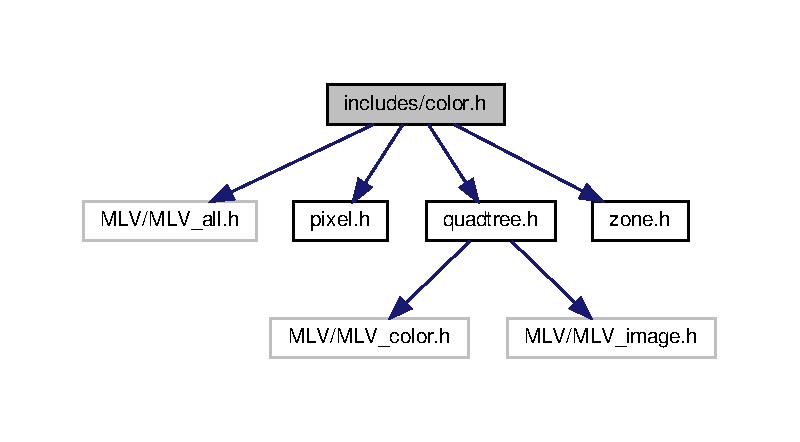
\includegraphics[width=350pt]{color_8h__incl}
\end{center}
\end{figure}
This graph shows which files directly or indirectly include this file\+:
\nopagebreak
\begin{figure}[H]
\begin{center}
\leavevmode
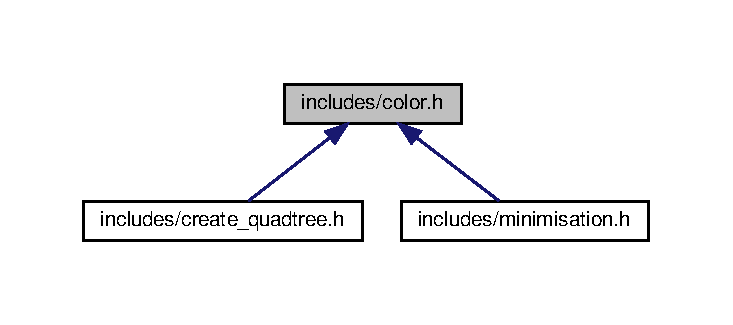
\includegraphics[width=350pt]{color_8h__dep__incl}
\end{center}
\end{figure}
\subsection*{Macros}
\begin{DoxyCompactItemize}
\item 
\#define \hyperlink{color_8h_a9bcb77d5a0957570f2eda790bf9caa4f}{M\+A\+X\+\_\+\+D\+I\+S\+T\+\_\+\+C\+O\+L\+OR}~20
\end{DoxyCompactItemize}
\subsection*{Functions}
\begin{DoxyCompactItemize}
\item 
int \hyperlink{color_8h_aba957ff783909eccd3e4ed1795275ba4}{kids\+\_\+same\+\_\+color} (\hyperlink{quadtree_8h_a184f2f10109642ad84b5619bcc5738da}{Tree} $\ast$t)
\begin{DoxyCompactList}\small\item\em Check if all t leaf have the same color. \end{DoxyCompactList}\item 
int \hyperlink{color_8h_ae352fca155d17554692045bee0f1f7d5}{close\+\_\+color} (M\+L\+V\+\_\+\+Color c1, M\+L\+V\+\_\+\+Color c2)
\begin{DoxyCompactList}\small\item\em Check if c1 and c2 have a close color. \end{DoxyCompactList}\item 
double \hyperlink{color_8h_ad1098571331055e832a1f6e547e14234}{color\+\_\+distance} (M\+L\+V\+\_\+\+Color c1, M\+L\+V\+\_\+\+Color c2)
\begin{DoxyCompactList}\small\item\em Calculates distance between 2 M\+L\+V\+\_\+\+Color. \end{DoxyCompactList}\item 
double \hyperlink{color_8h_ababfb6f80a6fbacb64bd92c40630f23a}{zone\+\_\+color\+\_\+error} (M\+L\+V\+\_\+\+Color zone\+\_\+color, const M\+L\+V\+\_\+\+Image $\ast$image, \hyperlink{structZone}{Zone} zone)
\begin{DoxyCompactList}\small\item\em Returns the error of a zone (= rectangle of top left corner (x1, y1), and bottom right corner (x2, y2)) \end{DoxyCompactList}\item 
M\+L\+V\+\_\+\+Color \hyperlink{color_8h_a73b7f54f2629977e1c67caaa2d843e17}{zone\+\_\+average\+\_\+color} (const M\+L\+V\+\_\+\+Image $\ast$image, \hyperlink{structZone}{Zone} zone)
\begin{DoxyCompactList}\small\item\em Returns the average color of a zone (= rectangle of top left corner (x1, y1) and bottom right corner (x2, y2)) \end{DoxyCompactList}\item 
void \hyperlink{color_8h_a997d12f58e17dcb91c80954899cb2943}{get\+\_\+zones\+\_\+average\+\_\+color} (const M\+L\+V\+\_\+\+Image $\ast$image, \hyperlink{structZone}{Zone} zone, M\+L\+V\+\_\+\+Color $\ast$no, M\+L\+V\+\_\+\+Color $\ast$ne, M\+L\+V\+\_\+\+Color $\ast$so, M\+L\+V\+\_\+\+Color $\ast$se)
\begin{DoxyCompactList}\small\item\em Subdivise a zone to get all its zones (NO, NE, SE, SO) average color. \end{DoxyCompactList}\end{DoxyCompactItemize}


\subsection{Macro Definition Documentation}
\mbox{\Hypertarget{color_8h_a9bcb77d5a0957570f2eda790bf9caa4f}\label{color_8h_a9bcb77d5a0957570f2eda790bf9caa4f}} 
\index{color.\+h@{color.\+h}!M\+A\+X\+\_\+\+D\+I\+S\+T\+\_\+\+C\+O\+L\+OR@{M\+A\+X\+\_\+\+D\+I\+S\+T\+\_\+\+C\+O\+L\+OR}}
\index{M\+A\+X\+\_\+\+D\+I\+S\+T\+\_\+\+C\+O\+L\+OR@{M\+A\+X\+\_\+\+D\+I\+S\+T\+\_\+\+C\+O\+L\+OR}!color.\+h@{color.\+h}}
\subsubsection{\texorpdfstring{M\+A\+X\+\_\+\+D\+I\+S\+T\+\_\+\+C\+O\+L\+OR}{MAX\_DIST\_COLOR}}
{\footnotesize\ttfamily \#define M\+A\+X\+\_\+\+D\+I\+S\+T\+\_\+\+C\+O\+L\+OR~20}



\subsection{Function Documentation}
\mbox{\Hypertarget{color_8h_ae352fca155d17554692045bee0f1f7d5}\label{color_8h_ae352fca155d17554692045bee0f1f7d5}} 
\index{color.\+h@{color.\+h}!close\+\_\+color@{close\+\_\+color}}
\index{close\+\_\+color@{close\+\_\+color}!color.\+h@{color.\+h}}
\subsubsection{\texorpdfstring{close\+\_\+color()}{close\_color()}}
{\footnotesize\ttfamily int close\+\_\+color (\begin{DoxyParamCaption}\item[{M\+L\+V\+\_\+\+Color}]{c1,  }\item[{M\+L\+V\+\_\+\+Color}]{c2 }\end{DoxyParamCaption})}



Check if c1 and c2 have a close color. 


\begin{DoxyParams}{Parameters}
{\em c1} & The first M\+L\+V\+\_\+\+Color \\
\hline
{\em c2} & The second M\+L\+V\+\_\+\+Color \\
\hline
\end{DoxyParams}
\begin{DoxyReturn}{Returns}
1 if c1 an c2 r, g, b values are close enough, maximum of M\+A\+X\+\_\+\+D\+I\+S\+T\+\_\+\+C\+O\+L\+OR 0 otherwise 
\end{DoxyReturn}
\mbox{\Hypertarget{color_8h_ad1098571331055e832a1f6e547e14234}\label{color_8h_ad1098571331055e832a1f6e547e14234}} 
\index{color.\+h@{color.\+h}!color\+\_\+distance@{color\+\_\+distance}}
\index{color\+\_\+distance@{color\+\_\+distance}!color.\+h@{color.\+h}}
\subsubsection{\texorpdfstring{color\+\_\+distance()}{color\_distance()}}
{\footnotesize\ttfamily double color\+\_\+distance (\begin{DoxyParamCaption}\item[{M\+L\+V\+\_\+\+Color}]{c1,  }\item[{M\+L\+V\+\_\+\+Color}]{c2 }\end{DoxyParamCaption})}



Calculates distance between 2 M\+L\+V\+\_\+\+Color. 


\begin{DoxyParams}{Parameters}
{\em c1} & The first M\+L\+V\+\_\+\+Color \\
\hline
{\em c2} & The second M\+L\+V\+\_\+\+Color \\
\hline
\end{DoxyParams}
\begin{DoxyReturn}{Returns}
Distance between both colors 
\end{DoxyReturn}
\mbox{\Hypertarget{color_8h_a997d12f58e17dcb91c80954899cb2943}\label{color_8h_a997d12f58e17dcb91c80954899cb2943}} 
\index{color.\+h@{color.\+h}!get\+\_\+zones\+\_\+average\+\_\+color@{get\+\_\+zones\+\_\+average\+\_\+color}}
\index{get\+\_\+zones\+\_\+average\+\_\+color@{get\+\_\+zones\+\_\+average\+\_\+color}!color.\+h@{color.\+h}}
\subsubsection{\texorpdfstring{get\+\_\+zones\+\_\+average\+\_\+color()}{get\_zones\_average\_color()}}
{\footnotesize\ttfamily void get\+\_\+zones\+\_\+average\+\_\+color (\begin{DoxyParamCaption}\item[{const M\+L\+V\+\_\+\+Image $\ast$}]{image,  }\item[{\hyperlink{structZone}{Zone}}]{zone,  }\item[{M\+L\+V\+\_\+\+Color $\ast$}]{no,  }\item[{M\+L\+V\+\_\+\+Color $\ast$}]{ne,  }\item[{M\+L\+V\+\_\+\+Color $\ast$}]{so,  }\item[{M\+L\+V\+\_\+\+Color $\ast$}]{se }\end{DoxyParamCaption})}



Subdivise a zone to get all its zones (NO, NE, SE, SO) average color. 


\begin{DoxyParams}{Parameters}
{\em image} & The image we\textquotesingle{}ll calculate each zone\textquotesingle{}s average color \\
\hline
{\em zone} & The zone we are subdivising \\
\hline
{\em no} & NO zone of parameter \char`\"{}zone\char`\"{} \\
\hline
{\em ne} & NE zone of parameter \char`\"{}zone\char`\"{} \\
\hline
{\em so} & SO zone of parameter \char`\"{}zone\char`\"{} \\
\hline
{\em se} & SE zone of parameter \char`\"{}zone\char`\"{} \\
\hline
\end{DoxyParams}
\mbox{\Hypertarget{color_8h_aba957ff783909eccd3e4ed1795275ba4}\label{color_8h_aba957ff783909eccd3e4ed1795275ba4}} 
\index{color.\+h@{color.\+h}!kids\+\_\+same\+\_\+color@{kids\+\_\+same\+\_\+color}}
\index{kids\+\_\+same\+\_\+color@{kids\+\_\+same\+\_\+color}!color.\+h@{color.\+h}}
\subsubsection{\texorpdfstring{kids\+\_\+same\+\_\+color()}{kids\_same\_color()}}
{\footnotesize\ttfamily int kids\+\_\+same\+\_\+color (\begin{DoxyParamCaption}\item[{\hyperlink{quadtree_8h_a184f2f10109642ad84b5619bcc5738da}{Tree} $\ast$}]{t }\end{DoxyParamCaption})}



Check if all t leaf have the same color. 


\begin{DoxyParams}{Parameters}
{\em t} & The tree we are looking at \\
\hline
\end{DoxyParams}
\begin{DoxyReturn}{Returns}
1 if all its leaf have the same color 0 otherwise 
\end{DoxyReturn}
\mbox{\Hypertarget{color_8h_a73b7f54f2629977e1c67caaa2d843e17}\label{color_8h_a73b7f54f2629977e1c67caaa2d843e17}} 
\index{color.\+h@{color.\+h}!zone\+\_\+average\+\_\+color@{zone\+\_\+average\+\_\+color}}
\index{zone\+\_\+average\+\_\+color@{zone\+\_\+average\+\_\+color}!color.\+h@{color.\+h}}
\subsubsection{\texorpdfstring{zone\+\_\+average\+\_\+color()}{zone\_average\_color()}}
{\footnotesize\ttfamily M\+L\+V\+\_\+\+Color zone\+\_\+average\+\_\+color (\begin{DoxyParamCaption}\item[{const M\+L\+V\+\_\+\+Image $\ast$}]{image,  }\item[{\hyperlink{structZone}{Zone}}]{zone }\end{DoxyParamCaption})}



Returns the average color of a zone (= rectangle of top left corner (x1, y1) and bottom right corner (x2, y2)) 


\begin{DoxyParams}{Parameters}
{\em image} & The image we are calculating the error from \\
\hline
{\em zone} & The zone we are calculating the error from \\
\hline
\end{DoxyParams}
\begin{DoxyReturn}{Returns}
The M\+L\+V\+\_\+\+Color of the zone 
\end{DoxyReturn}
\mbox{\Hypertarget{color_8h_ababfb6f80a6fbacb64bd92c40630f23a}\label{color_8h_ababfb6f80a6fbacb64bd92c40630f23a}} 
\index{color.\+h@{color.\+h}!zone\+\_\+color\+\_\+error@{zone\+\_\+color\+\_\+error}}
\index{zone\+\_\+color\+\_\+error@{zone\+\_\+color\+\_\+error}!color.\+h@{color.\+h}}
\subsubsection{\texorpdfstring{zone\+\_\+color\+\_\+error()}{zone\_color\_error()}}
{\footnotesize\ttfamily double zone\+\_\+color\+\_\+error (\begin{DoxyParamCaption}\item[{M\+L\+V\+\_\+\+Color}]{zone\+\_\+color,  }\item[{const M\+L\+V\+\_\+\+Image $\ast$}]{image,  }\item[{\hyperlink{structZone}{Zone}}]{zone }\end{DoxyParamCaption})}



Returns the error of a zone (= rectangle of top left corner (x1, y1), and bottom right corner (x2, y2)) 


\begin{DoxyParams}{Parameters}
{\em zone\+\_\+color} & \hyperlink{structZone}{Zone}\textquotesingle{}s color \\
\hline
{\em image} & The image we are calculating the error from \\
\hline
{\em zone} & The zone we are calculating the error from \\
\hline
\end{DoxyParams}
\begin{DoxyReturn}{Returns}
The error from the zone 
\end{DoxyReturn}

\hypertarget{create__quadtree_8h}{}\section{includes/create\+\_\+quadtree.h File Reference}
\label{create__quadtree_8h}\index{includes/create\+\_\+quadtree.\+h@{includes/create\+\_\+quadtree.\+h}}
{\ttfamily \#include \char`\"{}color.\+h\char`\"{}}\newline
{\ttfamily \#include \char`\"{}list\+\_\+errors.\+h\char`\"{}}\newline
{\ttfamily \#include \char`\"{}quadtree.\+h\char`\"{}}\newline
{\ttfamily \#include \char`\"{}zone.\+h\char`\"{}}\newline
Include dependency graph for create\+\_\+quadtree.\+h\+:
\nopagebreak
\begin{figure}[H]
\begin{center}
\leavevmode
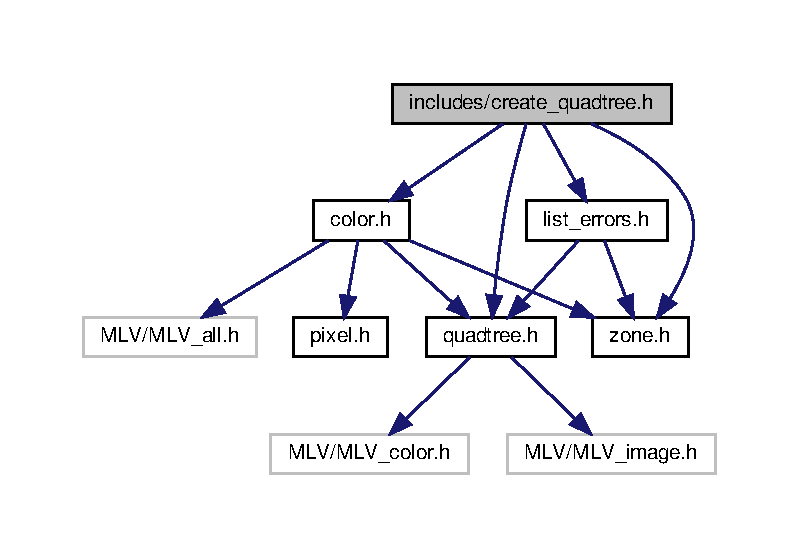
\includegraphics[width=350pt]{create__quadtree_8h__incl}
\end{center}
\end{figure}
\subsection*{Functions}
\begin{DoxyCompactItemize}
\item 
int \hyperlink{create__quadtree_8h_a8c1b0fdfc626727ca3e8f31b0f4af1e9}{create\+\_\+quadtree} (\hyperlink{quadtree_8h_a184f2f10109642ad84b5619bcc5738da}{Tree} $\ast$$\ast$t, M\+L\+V\+\_\+\+Image $\ast$image, \hyperlink{structErrorList__FirstLast}{Error\+List\+\_\+\+First\+Last} $\ast$list\+\_\+errors)
\begin{DoxyCompactList}\small\item\em Create a quadtree from scratch based on an image. \end{DoxyCompactList}\end{DoxyCompactItemize}


\subsection{Function Documentation}
\mbox{\Hypertarget{create__quadtree_8h_a8c1b0fdfc626727ca3e8f31b0f4af1e9}\label{create__quadtree_8h_a8c1b0fdfc626727ca3e8f31b0f4af1e9}} 
\index{create\+\_\+quadtree.\+h@{create\+\_\+quadtree.\+h}!create\+\_\+quadtree@{create\+\_\+quadtree}}
\index{create\+\_\+quadtree@{create\+\_\+quadtree}!create\+\_\+quadtree.\+h@{create\+\_\+quadtree.\+h}}
\subsubsection{\texorpdfstring{create\+\_\+quadtree()}{create\_quadtree()}}
{\footnotesize\ttfamily int create\+\_\+quadtree (\begin{DoxyParamCaption}\item[{\hyperlink{quadtree_8h_a184f2f10109642ad84b5619bcc5738da}{Tree} $\ast$$\ast$}]{t,  }\item[{M\+L\+V\+\_\+\+Image $\ast$}]{image,  }\item[{\hyperlink{structErrorList__FirstLast}{Error\+List\+\_\+\+First\+Last} $\ast$}]{list\+\_\+errors }\end{DoxyParamCaption})}



Create a quadtree from scratch based on an image. 


\begin{DoxyParams}{Parameters}
{\em t} & The quadtree we\textquotesingle{}ll create \\
\hline
{\em image} & The image we\textquotesingle{}ll create the quadtree from \\
\hline
{\em list\+\_\+errors} & All errors value from quadtree\textquotesingle{}s leaf \\
\hline
\end{DoxyParams}
\begin{DoxyReturn}{Returns}
-\/1 if we couldn\textquotesingle{}t create the quadtree 1 if the quadtree was created 
\end{DoxyReturn}

\hypertarget{decoding_8h}{}\section{includes/decoding.h File Reference}
\label{decoding_8h}\index{includes/decoding.\+h@{includes/decoding.\+h}}
{\ttfamily \#include $<$M\+L\+V/\+M\+L\+V\+\_\+all.\+h$>$}\newline
{\ttfamily \#include \char`\"{}bit\+\_\+buffer.\+h\char`\"{}}\newline
{\ttfamily \#include \char`\"{}quadtree.\+h\char`\"{}}\newline
Include dependency graph for decoding.\+h\+:
\nopagebreak
\begin{figure}[H]
\begin{center}
\leavevmode
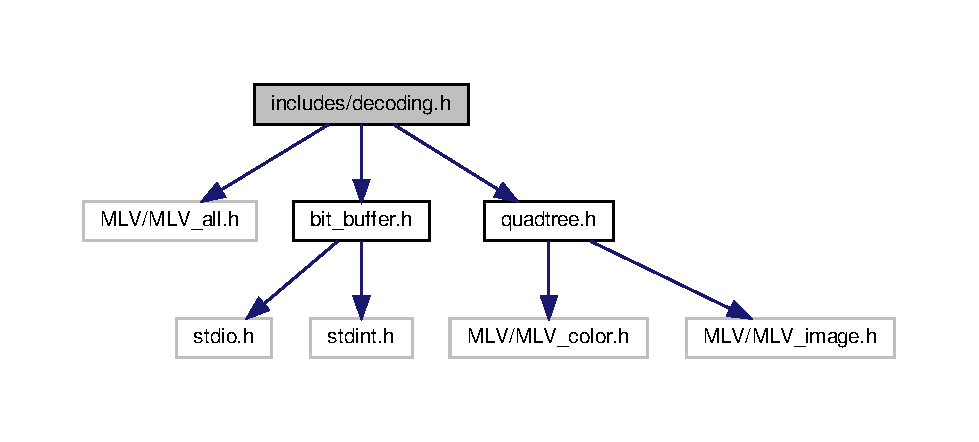
\includegraphics[width=350pt]{decoding_8h__incl}
\end{center}
\end{figure}
This graph shows which files directly or indirectly include this file\+:
\nopagebreak
\begin{figure}[H]
\begin{center}
\leavevmode
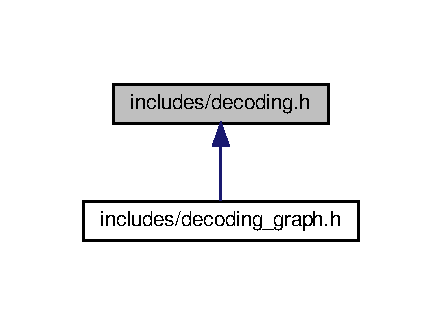
\includegraphics[width=212pt]{decoding_8h__dep__incl}
\end{center}
\end{figure}
\subsection*{Functions}
\begin{DoxyCompactItemize}
\item 
int \hyperlink{decoding_8h_ad9f760fae273a7a242bf2fc78d6dc5e8}{new\+\_\+node\+\_\+decoding} (\hyperlink{quadtree_8h_a184f2f10109642ad84b5619bcc5738da}{Tree} $\ast$$\ast$node)
\begin{DoxyCompactList}\small\item\em Allocate a tree with its type == N\+O\+DE, and without calculating any of its field (color\+\_\+error or subtree (color/leafs)) \end{DoxyCompactList}\item 
int \hyperlink{decoding_8h_a86c16c72de4c33bf0dbf49cd72e2131b}{new\+\_\+leaf\+\_\+decoding} (\hyperlink{quadtree_8h_a184f2f10109642ad84b5619bcc5738da}{Tree} $\ast$$\ast$leaf)
\begin{DoxyCompactList}\small\item\em Allocate a tree with its type == L\+E\+AF, and without calculating any of its field (color\+\_\+error or subtree (color/leafs)) \end{DoxyCompactList}\item 
int \hyperlink{decoding_8h_afdd371506a08147d6c1c8f4393c206ee}{decode\+\_\+tree} (\hyperlink{quadtree_8h_a184f2f10109642ad84b5619bcc5738da}{Tree} $\ast$$\ast$t, F\+I\+LE $\ast$file, int colored\+\_\+version)
\begin{DoxyCompactList}\small\item\em Read an encoded file (.qtc or .qtn) to fill a quadtree. \end{DoxyCompactList}\end{DoxyCompactItemize}


\subsection{Function Documentation}
\mbox{\Hypertarget{decoding_8h_afdd371506a08147d6c1c8f4393c206ee}\label{decoding_8h_afdd371506a08147d6c1c8f4393c206ee}} 
\index{decoding.\+h@{decoding.\+h}!decode\+\_\+tree@{decode\+\_\+tree}}
\index{decode\+\_\+tree@{decode\+\_\+tree}!decoding.\+h@{decoding.\+h}}
\subsubsection{\texorpdfstring{decode\+\_\+tree()}{decode\_tree()}}
{\footnotesize\ttfamily int decode\+\_\+tree (\begin{DoxyParamCaption}\item[{\hyperlink{quadtree_8h_a184f2f10109642ad84b5619bcc5738da}{Tree} $\ast$$\ast$}]{t,  }\item[{F\+I\+LE $\ast$}]{file,  }\item[{int}]{colored\+\_\+version }\end{DoxyParamCaption})}



Read an encoded file (.qtc or .qtn) to fill a quadtree. 


\begin{DoxyParams}{Parameters}
{\em t} & The tree we are filling \\
\hline
{\em file} & The file we are decoding \\
\hline
{\em colored\+\_\+version} & Whether we decode a tree in color or in B\&W (resp. 1 or 0) \\
\hline
\end{DoxyParams}
\begin{DoxyReturn}{Returns}
-\/4 If we couldn\textquotesingle{}t decode a color -\/3 If we coudn\textquotesingle{}t allocate a leaf -\/2 If we coudn\textquotesingle{}t allocate a node -\/1 If we coudn\textquotesingle{}t know wheter next tree will be a node or a leaf (file not correctly writed) 0 if we could decode file 
\end{DoxyReturn}
\mbox{\Hypertarget{decoding_8h_a86c16c72de4c33bf0dbf49cd72e2131b}\label{decoding_8h_a86c16c72de4c33bf0dbf49cd72e2131b}} 
\index{decoding.\+h@{decoding.\+h}!new\+\_\+leaf\+\_\+decoding@{new\+\_\+leaf\+\_\+decoding}}
\index{new\+\_\+leaf\+\_\+decoding@{new\+\_\+leaf\+\_\+decoding}!decoding.\+h@{decoding.\+h}}
\subsubsection{\texorpdfstring{new\+\_\+leaf\+\_\+decoding()}{new\_leaf\_decoding()}}
{\footnotesize\ttfamily int new\+\_\+leaf\+\_\+decoding (\begin{DoxyParamCaption}\item[{\hyperlink{quadtree_8h_a184f2f10109642ad84b5619bcc5738da}{Tree} $\ast$$\ast$}]{leaf }\end{DoxyParamCaption})}



Allocate a tree with its type == L\+E\+AF, and without calculating any of its field (color\+\_\+error or subtree (color/leafs)) 


\begin{DoxyParams}{Parameters}
{\em node} & The tree we are allocating \\
\hline
\end{DoxyParams}
\begin{DoxyReturn}{Returns}
-\/1 if we couldn\textquotesingle{}t allocate the tree -\/2 if we couldn\textquotesingle{}t allocate tree\textquotesingle{}s subtree 1 if we allocate the tree without any problem 
\end{DoxyReturn}
\mbox{\Hypertarget{decoding_8h_ad9f760fae273a7a242bf2fc78d6dc5e8}\label{decoding_8h_ad9f760fae273a7a242bf2fc78d6dc5e8}} 
\index{decoding.\+h@{decoding.\+h}!new\+\_\+node\+\_\+decoding@{new\+\_\+node\+\_\+decoding}}
\index{new\+\_\+node\+\_\+decoding@{new\+\_\+node\+\_\+decoding}!decoding.\+h@{decoding.\+h}}
\subsubsection{\texorpdfstring{new\+\_\+node\+\_\+decoding()}{new\_node\_decoding()}}
{\footnotesize\ttfamily int new\+\_\+node\+\_\+decoding (\begin{DoxyParamCaption}\item[{\hyperlink{quadtree_8h_a184f2f10109642ad84b5619bcc5738da}{Tree} $\ast$$\ast$}]{node }\end{DoxyParamCaption})}



Allocate a tree with its type == N\+O\+DE, and without calculating any of its field (color\+\_\+error or subtree (color/leafs)) 


\begin{DoxyParams}{Parameters}
{\em node} & The tree we are allocating \\
\hline
\end{DoxyParams}
\begin{DoxyReturn}{Returns}
-\/1 if we couldn\textquotesingle{}t allocate the tree -\/2 if we couldn\textquotesingle{}t allocate tree\textquotesingle{}s subtree 1 if we allocate the tree without any problem 
\end{DoxyReturn}

\hypertarget{decoding__graph_8h}{}\section{includes/decoding\+\_\+graph.h File Reference}
\label{decoding__graph_8h}\index{includes/decoding\+\_\+graph.\+h@{includes/decoding\+\_\+graph.\+h}}
{\ttfamily \#include $<$M\+L\+V/\+M\+L\+V\+\_\+all.\+h$>$}\newline
{\ttfamily \#include \char`\"{}decoding.\+h\char`\"{}}\newline
{\ttfamily \#include \char`\"{}quadtree.\+h\char`\"{}}\newline
Include dependency graph for decoding\+\_\+graph.\+h\+:
\nopagebreak
\begin{figure}[H]
\begin{center}
\leavevmode
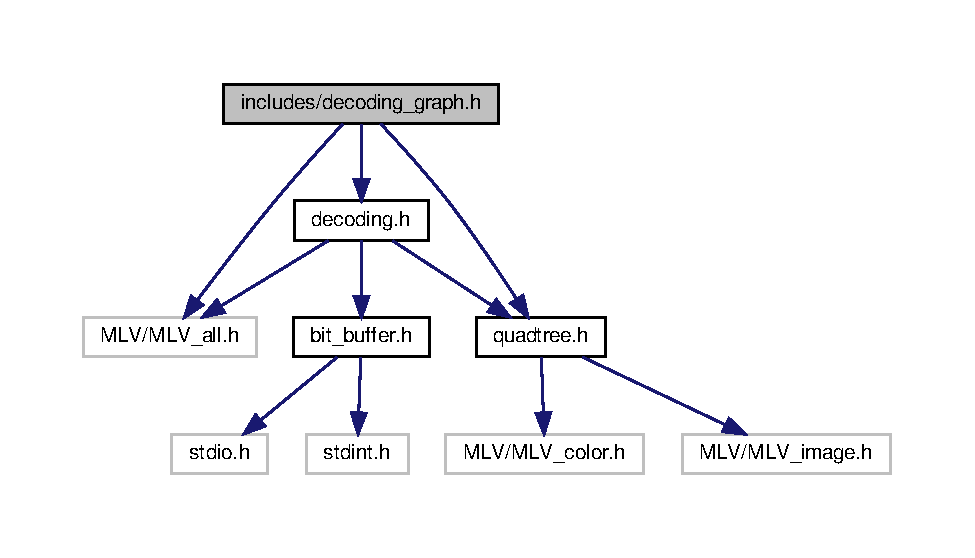
\includegraphics[width=350pt]{decoding__graph_8h__incl}
\end{center}
\end{figure}
\subsection*{Functions}
\begin{DoxyCompactItemize}
\item 
int \hyperlink{decoding__graph_8h_ad5c243dcdbedd8d87cd425631bdb44f6}{decoding\+\_\+graph} (\hyperlink{quadtree_8h_a184f2f10109642ad84b5619bcc5738da}{Tree} $\ast$$\ast$t, F\+I\+LE $\ast$file)
\begin{DoxyCompactList}\small\item\em Read an encoded colored graph file (.gmc) to fill a quadtree. \end{DoxyCompactList}\item 
int \hyperlink{decoding__graph_8h_a81c1be8d0a41cd7b1724eb8e3dd482fd}{decoding\+\_\+graph\+\_\+bw} (\hyperlink{quadtree_8h_a184f2f10109642ad84b5619bcc5738da}{Tree} $\ast$$\ast$t, F\+I\+LE $\ast$file)
\begin{DoxyCompactList}\small\item\em Read an encoded B\&W graph file (.gmn) to fill a quadtree. \end{DoxyCompactList}\end{DoxyCompactItemize}


\subsection{Function Documentation}
\mbox{\Hypertarget{decoding__graph_8h_ad5c243dcdbedd8d87cd425631bdb44f6}\label{decoding__graph_8h_ad5c243dcdbedd8d87cd425631bdb44f6}} 
\index{decoding\+\_\+graph.\+h@{decoding\+\_\+graph.\+h}!decoding\+\_\+graph@{decoding\+\_\+graph}}
\index{decoding\+\_\+graph@{decoding\+\_\+graph}!decoding\+\_\+graph.\+h@{decoding\+\_\+graph.\+h}}
\subsubsection{\texorpdfstring{decoding\+\_\+graph()}{decoding\_graph()}}
{\footnotesize\ttfamily int decoding\+\_\+graph (\begin{DoxyParamCaption}\item[{\hyperlink{quadtree_8h_a184f2f10109642ad84b5619bcc5738da}{Tree} $\ast$$\ast$}]{t,  }\item[{F\+I\+LE $\ast$}]{file }\end{DoxyParamCaption})}



Read an encoded colored graph file (.gmc) to fill a quadtree. 


\begin{DoxyParams}{Parameters}
{\em t} & The tree we are filling \\
\hline
{\em file} & The file we are decoding \\
\hline
\end{DoxyParams}
\begin{DoxyReturn}{Returns}
-\/4 if the last character of the first string from the file wasn\textquotesingle{}t correctly writed (not a digit, nor \textquotesingle{}f\textquotesingle{}) -\/3 if a color wasn\textquotesingle{}t correctly writed (r, g, b or a $<$ 0 or $>$ 255) -\/2 if a leaf couldn\textquotesingle{}t be allocated -\/1 if a node couldn\textquotesingle{}t be allocated 0 if it worked 
\end{DoxyReturn}
\mbox{\Hypertarget{decoding__graph_8h_a81c1be8d0a41cd7b1724eb8e3dd482fd}\label{decoding__graph_8h_a81c1be8d0a41cd7b1724eb8e3dd482fd}} 
\index{decoding\+\_\+graph.\+h@{decoding\+\_\+graph.\+h}!decoding\+\_\+graph\+\_\+bw@{decoding\+\_\+graph\+\_\+bw}}
\index{decoding\+\_\+graph\+\_\+bw@{decoding\+\_\+graph\+\_\+bw}!decoding\+\_\+graph.\+h@{decoding\+\_\+graph.\+h}}
\subsubsection{\texorpdfstring{decoding\+\_\+graph\+\_\+bw()}{decoding\_graph\_bw()}}
{\footnotesize\ttfamily int decoding\+\_\+graph\+\_\+bw (\begin{DoxyParamCaption}\item[{\hyperlink{quadtree_8h_a184f2f10109642ad84b5619bcc5738da}{Tree} $\ast$$\ast$}]{t,  }\item[{F\+I\+LE $\ast$}]{file }\end{DoxyParamCaption})}



Read an encoded B\&W graph file (.gmn) to fill a quadtree. 


\begin{DoxyParams}{Parameters}
{\em t} & The tree we are filling \\
\hline
{\em file} & The file we are decoding \\
\hline
\end{DoxyParams}
\begin{DoxyReturn}{Returns}
-\/4 if the last character of the first string from the file wasn\textquotesingle{}t correctly writed (not a digit, nor \textquotesingle{}f\textquotesingle{}) -\/3 if a color wasn\textquotesingle{}t correctly writed (r, g, b or a $<$ 0 or $>$ 255) -\/2 if a leaf couldn\textquotesingle{}t be allocated -\/1 if a node couldn\textquotesingle{}t be allocated 0 if it worked 
\end{DoxyReturn}

\hypertarget{encoding_8h}{}\section{includes/encoding.h File Reference}
\label{encoding_8h}\index{includes/encoding.\+h@{includes/encoding.\+h}}
{\ttfamily \#include $<$M\+L\+V/\+M\+L\+V\+\_\+all.\+h$>$}\newline
{\ttfamily \#include \char`\"{}bit\+\_\+buffer.\+h\char`\"{}}\newline
{\ttfamily \#include \char`\"{}quadtree.\+h\char`\"{}}\newline
Include dependency graph for encoding.\+h\+:
\nopagebreak
\begin{figure}[H]
\begin{center}
\leavevmode
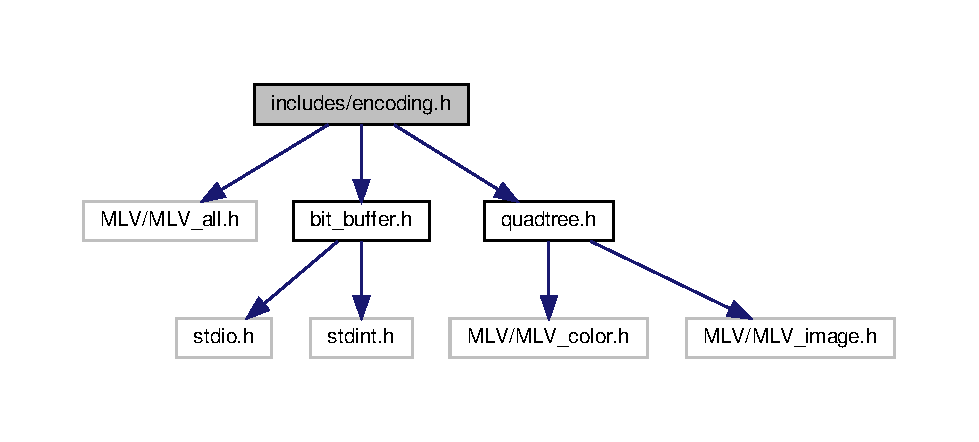
\includegraphics[width=350pt]{encoding_8h__incl}
\end{center}
\end{figure}
\subsection*{Functions}
\begin{DoxyCompactItemize}
\item 
void \hyperlink{encoding_8h_a8d006c5e54e049ac9493a95ab5ad9893}{encode\+\_\+tree} (\hyperlink{quadtree_8h_a184f2f10109642ad84b5619bcc5738da}{Tree} $\ast$t, F\+I\+LE $\ast$file, int colored\+\_\+version)
\begin{DoxyCompactList}\small\item\em Encode a (not minimized) quadtree in file. \end{DoxyCompactList}\end{DoxyCompactItemize}


\subsection{Function Documentation}
\mbox{\Hypertarget{encoding_8h_a8d006c5e54e049ac9493a95ab5ad9893}\label{encoding_8h_a8d006c5e54e049ac9493a95ab5ad9893}} 
\index{encoding.\+h@{encoding.\+h}!encode\+\_\+tree@{encode\+\_\+tree}}
\index{encode\+\_\+tree@{encode\+\_\+tree}!encoding.\+h@{encoding.\+h}}
\subsubsection{\texorpdfstring{encode\+\_\+tree()}{encode\_tree()}}
{\footnotesize\ttfamily void encode\+\_\+tree (\begin{DoxyParamCaption}\item[{\hyperlink{quadtree_8h_a184f2f10109642ad84b5619bcc5738da}{Tree} $\ast$}]{t,  }\item[{F\+I\+LE $\ast$}]{file,  }\item[{int}]{colored\+\_\+version }\end{DoxyParamCaption})}



Encode a (not minimized) quadtree in file. 


\begin{DoxyParams}{Parameters}
{\em t} & The quadtree we are encoding \\
\hline
{\em file} & The file we are using to encode t \\
\hline
{\em colored\+\_\+version} & Whether we encode a tree in color or in B\&W (resp. 1 or 0) \\
\hline
\end{DoxyParams}

\hypertarget{encoding__graph_8h}{}\section{includes/encoding\+\_\+graph.h File Reference}
\label{encoding__graph_8h}\index{includes/encoding\+\_\+graph.\+h@{includes/encoding\+\_\+graph.\+h}}
{\ttfamily \#include $<$M\+L\+V/\+M\+L\+V\+\_\+all.\+h$>$}\newline
{\ttfamily \#include \char`\"{}quadtree.\+h\char`\"{}}\newline
Include dependency graph for encoding\+\_\+graph.\+h\+:
\nopagebreak
\begin{figure}[H]
\begin{center}
\leavevmode
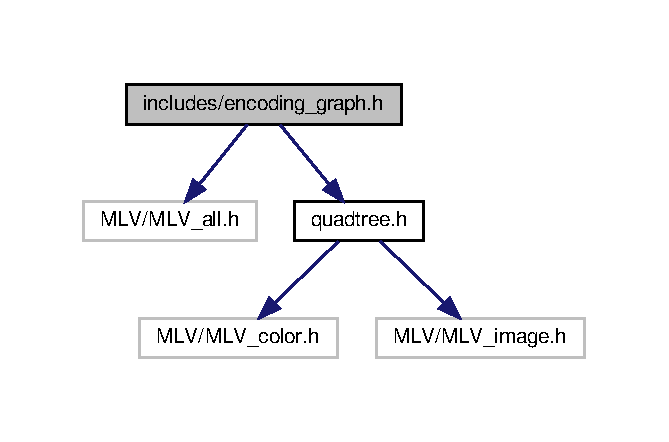
\includegraphics[width=321pt]{encoding__graph_8h__incl}
\end{center}
\end{figure}
\subsection*{Data Structures}
\begin{DoxyCompactItemize}
\item 
struct \hyperlink{structLeaf__nums}{Leaf\+\_\+nums}
\end{DoxyCompactItemize}
\subsection*{Functions}
\begin{DoxyCompactItemize}
\item 
int \hyperlink{encoding__graph_8h_a1c6d55f1fa15645ed8c12306abef58c3}{encoding\+\_\+graph} (\hyperlink{quadtree_8h_a184f2f10109642ad84b5619bcc5738da}{Tree} $\ast$t, F\+I\+LE $\ast$file, int current\+\_\+node, int node\+\_\+total)
\begin{DoxyCompactList}\small\item\em Encode a minimized quadtree (in color) \end{DoxyCompactList}\item 
int \hyperlink{encoding__graph_8h_aa4e667e49c732e5ac4047568bd943867}{encoding\+\_\+graph\+\_\+bw} (\hyperlink{quadtree_8h_a184f2f10109642ad84b5619bcc5738da}{Tree} $\ast$t, F\+I\+LE $\ast$file, int current\+\_\+node, int node\+\_\+total)
\begin{DoxyCompactList}\small\item\em Encode a minimized quadtree (in black \& white) \end{DoxyCompactList}\end{DoxyCompactItemize}


\subsection{Function Documentation}
\mbox{\Hypertarget{encoding__graph_8h_a1c6d55f1fa15645ed8c12306abef58c3}\label{encoding__graph_8h_a1c6d55f1fa15645ed8c12306abef58c3}} 
\index{encoding\+\_\+graph.\+h@{encoding\+\_\+graph.\+h}!encoding\+\_\+graph@{encoding\+\_\+graph}}
\index{encoding\+\_\+graph@{encoding\+\_\+graph}!encoding\+\_\+graph.\+h@{encoding\+\_\+graph.\+h}}
\subsubsection{\texorpdfstring{encoding\+\_\+graph()}{encoding\_graph()}}
{\footnotesize\ttfamily int encoding\+\_\+graph (\begin{DoxyParamCaption}\item[{\hyperlink{quadtree_8h_a184f2f10109642ad84b5619bcc5738da}{Tree} $\ast$}]{t,  }\item[{F\+I\+LE $\ast$}]{file,  }\item[{int}]{current\+\_\+node,  }\item[{int}]{node\+\_\+total }\end{DoxyParamCaption})}



Encode a minimized quadtree (in color) 


\begin{DoxyParams}{Parameters}
{\em t} & The tree we are encoding \\
\hline
{\em file} & The file we are using the encode t \\
\hline
{\em current\+\_\+node} & The number of the node we are encoding \\
\hline
{\em node\+\_\+total} & The number of node so far \\
\hline
\end{DoxyParams}
\begin{DoxyReturn}{Returns}
The number of node so far to actualize it (since it\textquotesingle{}s a recursive function) 
\end{DoxyReturn}
\mbox{\Hypertarget{encoding__graph_8h_aa4e667e49c732e5ac4047568bd943867}\label{encoding__graph_8h_aa4e667e49c732e5ac4047568bd943867}} 
\index{encoding\+\_\+graph.\+h@{encoding\+\_\+graph.\+h}!encoding\+\_\+graph\+\_\+bw@{encoding\+\_\+graph\+\_\+bw}}
\index{encoding\+\_\+graph\+\_\+bw@{encoding\+\_\+graph\+\_\+bw}!encoding\+\_\+graph.\+h@{encoding\+\_\+graph.\+h}}
\subsubsection{\texorpdfstring{encoding\+\_\+graph\+\_\+bw()}{encoding\_graph\_bw()}}
{\footnotesize\ttfamily int encoding\+\_\+graph\+\_\+bw (\begin{DoxyParamCaption}\item[{\hyperlink{quadtree_8h_a184f2f10109642ad84b5619bcc5738da}{Tree} $\ast$}]{t,  }\item[{F\+I\+LE $\ast$}]{file,  }\item[{int}]{current\+\_\+node,  }\item[{int}]{node\+\_\+total }\end{DoxyParamCaption})}



Encode a minimized quadtree (in black \& white) 


\begin{DoxyParams}{Parameters}
{\em t} & The tree we are encoding \\
\hline
{\em file} & The file we are using the encode t \\
\hline
{\em current\+\_\+node} & The number of the node we are encoding \\
\hline
{\em node\+\_\+total} & The number of node so far \\
\hline
\end{DoxyParams}
\begin{DoxyReturn}{Returns}
The number of node so far to actualize it (since it\textquotesingle{}s a recursive function) 
\end{DoxyReturn}

\hypertarget{io_8h}{}\section{includes/io.h File Reference}
\label{io_8h}\index{includes/io.\+h@{includes/io.\+h}}
{\ttfamily \#include \char`\"{}quadtree.\+h\char`\"{}}\newline
{\ttfamily \#include \char`\"{}list\+\_\+errors.\+h\char`\"{}}\newline
{\ttfamily \#include \char`\"{}window.\+h\char`\"{}}\newline
Include dependency graph for io.\+h\+:
\nopagebreak
\begin{figure}[H]
\begin{center}
\leavevmode
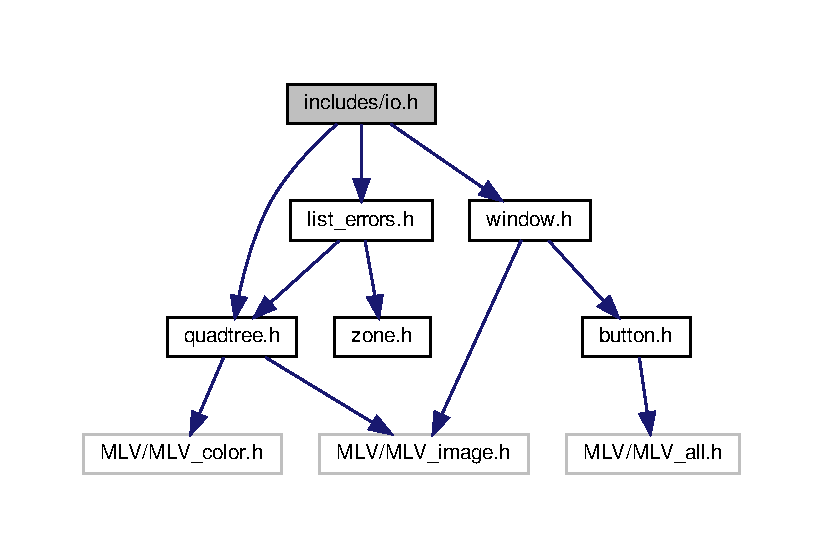
\includegraphics[width=350pt]{io_8h__incl}
\end{center}
\end{figure}
\subsection*{Macros}
\begin{DoxyCompactItemize}
\item 
\#define \hyperlink{io_8h_a9cc8659863c4248476caec5457ce3f3b}{B\+T\+N\+\_\+\+T\+X\+T\+\_\+1}~\char`\"{}open image\char`\"{}
\item 
\#define \hyperlink{io_8h_a066330c13795fda64550f995d091129b}{B\+T\+N\+\_\+\+T\+X\+T\+\_\+2}~\char`\"{}quadtree approximation\char`\"{}
\item 
\#define \hyperlink{io_8h_ac32a77b38fe1dc7a0e8ba15189f1a46a}{B\+T\+N\+\_\+\+T\+X\+T\+\_\+3}~\char`\"{}save rgba bianary\char`\"{}
\item 
\#define \hyperlink{io_8h_ab067263c99b0fffb72a15f7492451bda}{B\+T\+N\+\_\+\+T\+X\+T\+\_\+4}~\char`\"{}save b\&w binary\char`\"{}
\item 
\#define \hyperlink{io_8h_a3aa77fd4d081ceeb31fc038014157bc9}{B\+T\+N\+\_\+\+T\+X\+T\+\_\+5}~\char`\"{}minimisation with loss\char`\"{}
\item 
\#define \hyperlink{io_8h_a7d1d4d075486ed42bcf0dc4d4f762d17}{B\+T\+N\+\_\+\+T\+X\+T\+\_\+6}~\char`\"{}minimisation no loss\char`\"{}
\item 
\#define \hyperlink{io_8h_a3f1fa493a3bbfe6089813915a123387d}{B\+T\+N\+\_\+\+T\+X\+T\+\_\+7}~\char`\"{}save rgba graf\char`\"{}
\item 
\#define \hyperlink{io_8h_ac942e285d89c48ca7fae7aa30a4ec77c}{B\+T\+N\+\_\+\+T\+X\+T\+\_\+8}~\char`\"{}save b\&w graf\char`\"{}
\item 
\#define \hyperlink{io_8h_a5b8dd850afd22b935090b014c0a689f7}{B\+T\+N\+\_\+\+T\+X\+T\+\_\+9}~\char`\"{}quit\char`\"{}
\end{DoxyCompactItemize}
\subsection*{Enumerations}
\begin{DoxyCompactItemize}
\item 
enum \hyperlink{io_8h_a5f30136376402d67d35fc7b2e50983d9}{Verssion} \{ \newline
\hyperlink{io_8h_a5f30136376402d67d35fc7b2e50983d9a7e07130e0bea13162408021d61994021}{N\+O\+PE}, 
\hyperlink{io_8h_a5f30136376402d67d35fc7b2e50983d9a5a381b4eb702558ca3a9649c4e688793}{G\+R\+A\+P\+H\+\_\+\+BW}, 
\hyperlink{io_8h_a5f30136376402d67d35fc7b2e50983d9af42331660d769fa0d6d73f153ddea9c5}{G\+R\+A\+P\+H\+\_\+\+C\+O\+L\+OR}, 
\hyperlink{io_8h_a5f30136376402d67d35fc7b2e50983d9af0a4fadc79e905023dde32154a19818c}{Q\+U\+A\+D\+\_\+\+BW}, 
\newline
\hyperlink{io_8h_a5f30136376402d67d35fc7b2e50983d9af9b1d6f5461b858c009e41e49af50507}{Q\+U\+A\+D\+\_\+\+C\+O\+L\+OR}, 
\hyperlink{io_8h_a5f30136376402d67d35fc7b2e50983d9a690e276cddb6f613322ac8bbc9ae967a}{S\+T\+D\+\_\+\+I\+M\+A\+GE}
 \}
\item 
enum \hyperlink{io_8h_a369a6fddbb0e74817c96573ea88b9d9d}{Button\+\_\+fct} \{ \newline
\hyperlink{io_8h_a369a6fddbb0e74817c96573ea88b9d9daa4cec4073c0ed7580030ea1847a5c1de}{O\+P\+E\+N\+\_\+\+I\+M\+A\+GE}, 
\hyperlink{io_8h_a369a6fddbb0e74817c96573ea88b9d9daafc216f903382899676d177c546c1128}{Q\+U\+A\+D\+\_\+\+T\+R\+E\+E\+\_\+\+A\+P\+P\+R\+OX}, 
\hyperlink{io_8h_a369a6fddbb0e74817c96573ea88b9d9daae8f5377f4515c0353117febbcf24515}{S\+A\+V\+E\+\_\+\+Q\+U\+A\+D\+\_\+\+C\+O\+L\+OR}, 
\hyperlink{io_8h_a369a6fddbb0e74817c96573ea88b9d9da2db3e1881c0be00e2092e853546dd6e5}{S\+A\+V\+E\+\_\+\+Q\+U\+A\+D\+\_\+\+BW}, 
\newline
\hyperlink{io_8h_a369a6fddbb0e74817c96573ea88b9d9da7f1dbab2951cb886e4eb7fcc0f99a053}{M\+I\+N\+I\+M\+\_\+\+L\+O\+SS}, 
\hyperlink{io_8h_a369a6fddbb0e74817c96573ea88b9d9da64dec93d612b579b84194027f43fd875}{M\+I\+N\+I\+M\+\_\+\+N\+O\+\_\+\+L\+O\+SS}, 
\hyperlink{io_8h_a369a6fddbb0e74817c96573ea88b9d9daf1f539aa9d9c4a066f21e890fca44c56}{S\+A\+V\+E\+\_\+\+G\+R\+A\+P\+H\+\_\+\+C\+O\+L\+OR}, 
\hyperlink{io_8h_a369a6fddbb0e74817c96573ea88b9d9da6459d5c19ab64b688ef2732faef80960}{S\+A\+V\+E\+\_\+\+G\+R\+A\+P\+H\+\_\+\+BW}, 
\newline
\hyperlink{io_8h_a369a6fddbb0e74817c96573ea88b9d9da76bdc8adfd6c6463ab269ff4c06be9b4}{Q\+U\+IT}
 \}
\end{DoxyCompactItemize}
\subsection*{Functions}
\begin{DoxyCompactItemize}
\item 
void \hyperlink{io_8h_a768fad8da091c5289e0176189e7aeec1}{set\+\_\+button\+\_\+state\+\_\+quadtree\+\_\+bw} (\hyperlink{structButton}{Button} $\ast$array)
\begin{DoxyCompactList}\small\item\em This function changes the button state to fit the situation where a .qtn was loaded. \end{DoxyCompactList}\item 
void \hyperlink{io_8h_ab21fefacb448042f281751022e551f6d}{set\+\_\+button\+\_\+state\+\_\+no\+\_\+image} (\hyperlink{structButton}{Button} $\ast$array)
\begin{DoxyCompactList}\small\item\em This function changes the button state to fit the situation where a nothing was loaded. \end{DoxyCompactList}\item 
void \hyperlink{io_8h_a323b021e4079025caca68759aad876df}{set\+\_\+button\+\_\+state\+\_\+std\+\_\+image} (\hyperlink{structButton}{Button} $\ast$array)
\begin{DoxyCompactList}\small\item\em This function changes the button state to fit the situation where a standard image was loaded. \end{DoxyCompactList}\item 
void \hyperlink{io_8h_a4568e26282ca1e78c3527fa7a8fa954d}{set\+\_\+button\+\_\+state\+\_\+quadtree\+\_\+color} (\hyperlink{structButton}{Button} $\ast$array)
\begin{DoxyCompactList}\small\item\em This function changes the button state to fit the situation where a .qtc was loaded. \end{DoxyCompactList}\item 
void \hyperlink{io_8h_a96531291223b210721944c57b22063e4}{set\+\_\+button\+\_\+state\+\_\+graph\+\_\+bw} (\hyperlink{structButton}{Button} $\ast$array)
\begin{DoxyCompactList}\small\item\em This function changes the button state to fit the situation where a .gmn was loaded. \end{DoxyCompactList}\item 
void \hyperlink{io_8h_a16736344637a9f05174ee7a35a67b1be}{set\+\_\+button\+\_\+state\+\_\+graph\+\_\+color} (\hyperlink{structButton}{Button} $\ast$array)
\begin{DoxyCompactList}\small\item\em This function changes the button state to fit the situation where a .gmc was loaded. \end{DoxyCompactList}\item 
void \hyperlink{io_8h_a600dc79145181b397345c547320b5de2}{set\+\_\+was\+\_\+minimized\+\_\+no\+\_\+loss} (\hyperlink{structButton}{Button} $\ast$array)
\begin{DoxyCompactList}\small\item\em This function changes the button state to fit the situation where a quadtree was minimized without loss. \end{DoxyCompactList}\item 
void \hyperlink{io_8h_a253eb0d5474572333c1be40a23c1ac22}{set\+\_\+was\+\_\+minimized\+\_\+with\+\_\+loss} (\hyperlink{structButton}{Button} $\ast$array, \hyperlink{io_8h_a5f30136376402d67d35fc7b2e50983d9}{Verssion} verssion)
\begin{DoxyCompactList}\small\item\em This function changes the button state to fit the situation where a quadtree was minimized with loss. \end{DoxyCompactList}\item 
int \hyperlink{io_8h_a670d56bcb04709b69a4ae94fb886dfd8}{link\+\_\+btn} (int btn\+\_\+number, \hyperlink{structWin}{Win} $\ast$info, \hyperlink{quadtree_8h_a184f2f10109642ad84b5619bcc5738da}{Tree} $\ast$$\ast$t, \hyperlink{structErrorList__FirstLast}{Error\+List\+\_\+\+First\+Last} $\ast$color\+\_\+err\+\_\+list, \hyperlink{io_8h_a5f30136376402d67d35fc7b2e50983d9}{Verssion} $\ast$verssion)
\begin{DoxyCompactList}\small\item\em This function links the buttons to the functionalities they represents. \end{DoxyCompactList}\end{DoxyCompactItemize}


\subsection{Macro Definition Documentation}
\mbox{\Hypertarget{io_8h_a9cc8659863c4248476caec5457ce3f3b}\label{io_8h_a9cc8659863c4248476caec5457ce3f3b}} 
\index{io.\+h@{io.\+h}!B\+T\+N\+\_\+\+T\+X\+T\+\_\+1@{B\+T\+N\+\_\+\+T\+X\+T\+\_\+1}}
\index{B\+T\+N\+\_\+\+T\+X\+T\+\_\+1@{B\+T\+N\+\_\+\+T\+X\+T\+\_\+1}!io.\+h@{io.\+h}}
\subsubsection{\texorpdfstring{B\+T\+N\+\_\+\+T\+X\+T\+\_\+1}{BTN\_TXT\_1}}
{\footnotesize\ttfamily \#define B\+T\+N\+\_\+\+T\+X\+T\+\_\+1~\char`\"{}open image\char`\"{}}

\mbox{\Hypertarget{io_8h_a066330c13795fda64550f995d091129b}\label{io_8h_a066330c13795fda64550f995d091129b}} 
\index{io.\+h@{io.\+h}!B\+T\+N\+\_\+\+T\+X\+T\+\_\+2@{B\+T\+N\+\_\+\+T\+X\+T\+\_\+2}}
\index{B\+T\+N\+\_\+\+T\+X\+T\+\_\+2@{B\+T\+N\+\_\+\+T\+X\+T\+\_\+2}!io.\+h@{io.\+h}}
\subsubsection{\texorpdfstring{B\+T\+N\+\_\+\+T\+X\+T\+\_\+2}{BTN\_TXT\_2}}
{\footnotesize\ttfamily \#define B\+T\+N\+\_\+\+T\+X\+T\+\_\+2~\char`\"{}quadtree approximation\char`\"{}}

\mbox{\Hypertarget{io_8h_ac32a77b38fe1dc7a0e8ba15189f1a46a}\label{io_8h_ac32a77b38fe1dc7a0e8ba15189f1a46a}} 
\index{io.\+h@{io.\+h}!B\+T\+N\+\_\+\+T\+X\+T\+\_\+3@{B\+T\+N\+\_\+\+T\+X\+T\+\_\+3}}
\index{B\+T\+N\+\_\+\+T\+X\+T\+\_\+3@{B\+T\+N\+\_\+\+T\+X\+T\+\_\+3}!io.\+h@{io.\+h}}
\subsubsection{\texorpdfstring{B\+T\+N\+\_\+\+T\+X\+T\+\_\+3}{BTN\_TXT\_3}}
{\footnotesize\ttfamily \#define B\+T\+N\+\_\+\+T\+X\+T\+\_\+3~\char`\"{}save rgba bianary\char`\"{}}

\mbox{\Hypertarget{io_8h_ab067263c99b0fffb72a15f7492451bda}\label{io_8h_ab067263c99b0fffb72a15f7492451bda}} 
\index{io.\+h@{io.\+h}!B\+T\+N\+\_\+\+T\+X\+T\+\_\+4@{B\+T\+N\+\_\+\+T\+X\+T\+\_\+4}}
\index{B\+T\+N\+\_\+\+T\+X\+T\+\_\+4@{B\+T\+N\+\_\+\+T\+X\+T\+\_\+4}!io.\+h@{io.\+h}}
\subsubsection{\texorpdfstring{B\+T\+N\+\_\+\+T\+X\+T\+\_\+4}{BTN\_TXT\_4}}
{\footnotesize\ttfamily \#define B\+T\+N\+\_\+\+T\+X\+T\+\_\+4~\char`\"{}save b\&w binary\char`\"{}}

\mbox{\Hypertarget{io_8h_a3aa77fd4d081ceeb31fc038014157bc9}\label{io_8h_a3aa77fd4d081ceeb31fc038014157bc9}} 
\index{io.\+h@{io.\+h}!B\+T\+N\+\_\+\+T\+X\+T\+\_\+5@{B\+T\+N\+\_\+\+T\+X\+T\+\_\+5}}
\index{B\+T\+N\+\_\+\+T\+X\+T\+\_\+5@{B\+T\+N\+\_\+\+T\+X\+T\+\_\+5}!io.\+h@{io.\+h}}
\subsubsection{\texorpdfstring{B\+T\+N\+\_\+\+T\+X\+T\+\_\+5}{BTN\_TXT\_5}}
{\footnotesize\ttfamily \#define B\+T\+N\+\_\+\+T\+X\+T\+\_\+5~\char`\"{}minimisation with loss\char`\"{}}

\mbox{\Hypertarget{io_8h_a7d1d4d075486ed42bcf0dc4d4f762d17}\label{io_8h_a7d1d4d075486ed42bcf0dc4d4f762d17}} 
\index{io.\+h@{io.\+h}!B\+T\+N\+\_\+\+T\+X\+T\+\_\+6@{B\+T\+N\+\_\+\+T\+X\+T\+\_\+6}}
\index{B\+T\+N\+\_\+\+T\+X\+T\+\_\+6@{B\+T\+N\+\_\+\+T\+X\+T\+\_\+6}!io.\+h@{io.\+h}}
\subsubsection{\texorpdfstring{B\+T\+N\+\_\+\+T\+X\+T\+\_\+6}{BTN\_TXT\_6}}
{\footnotesize\ttfamily \#define B\+T\+N\+\_\+\+T\+X\+T\+\_\+6~\char`\"{}minimisation no loss\char`\"{}}

\mbox{\Hypertarget{io_8h_a3f1fa493a3bbfe6089813915a123387d}\label{io_8h_a3f1fa493a3bbfe6089813915a123387d}} 
\index{io.\+h@{io.\+h}!B\+T\+N\+\_\+\+T\+X\+T\+\_\+7@{B\+T\+N\+\_\+\+T\+X\+T\+\_\+7}}
\index{B\+T\+N\+\_\+\+T\+X\+T\+\_\+7@{B\+T\+N\+\_\+\+T\+X\+T\+\_\+7}!io.\+h@{io.\+h}}
\subsubsection{\texorpdfstring{B\+T\+N\+\_\+\+T\+X\+T\+\_\+7}{BTN\_TXT\_7}}
{\footnotesize\ttfamily \#define B\+T\+N\+\_\+\+T\+X\+T\+\_\+7~\char`\"{}save rgba graf\char`\"{}}

\mbox{\Hypertarget{io_8h_ac942e285d89c48ca7fae7aa30a4ec77c}\label{io_8h_ac942e285d89c48ca7fae7aa30a4ec77c}} 
\index{io.\+h@{io.\+h}!B\+T\+N\+\_\+\+T\+X\+T\+\_\+8@{B\+T\+N\+\_\+\+T\+X\+T\+\_\+8}}
\index{B\+T\+N\+\_\+\+T\+X\+T\+\_\+8@{B\+T\+N\+\_\+\+T\+X\+T\+\_\+8}!io.\+h@{io.\+h}}
\subsubsection{\texorpdfstring{B\+T\+N\+\_\+\+T\+X\+T\+\_\+8}{BTN\_TXT\_8}}
{\footnotesize\ttfamily \#define B\+T\+N\+\_\+\+T\+X\+T\+\_\+8~\char`\"{}save b\&w graf\char`\"{}}

\mbox{\Hypertarget{io_8h_a5b8dd850afd22b935090b014c0a689f7}\label{io_8h_a5b8dd850afd22b935090b014c0a689f7}} 
\index{io.\+h@{io.\+h}!B\+T\+N\+\_\+\+T\+X\+T\+\_\+9@{B\+T\+N\+\_\+\+T\+X\+T\+\_\+9}}
\index{B\+T\+N\+\_\+\+T\+X\+T\+\_\+9@{B\+T\+N\+\_\+\+T\+X\+T\+\_\+9}!io.\+h@{io.\+h}}
\subsubsection{\texorpdfstring{B\+T\+N\+\_\+\+T\+X\+T\+\_\+9}{BTN\_TXT\_9}}
{\footnotesize\ttfamily \#define B\+T\+N\+\_\+\+T\+X\+T\+\_\+9~\char`\"{}quit\char`\"{}}



\subsection{Enumeration Type Documentation}
\mbox{\Hypertarget{io_8h_a369a6fddbb0e74817c96573ea88b9d9d}\label{io_8h_a369a6fddbb0e74817c96573ea88b9d9d}} 
\index{io.\+h@{io.\+h}!Button\+\_\+fct@{Button\+\_\+fct}}
\index{Button\+\_\+fct@{Button\+\_\+fct}!io.\+h@{io.\+h}}
\subsubsection{\texorpdfstring{Button\+\_\+fct}{Button\_fct}}
{\footnotesize\ttfamily enum \hyperlink{io_8h_a369a6fddbb0e74817c96573ea88b9d9d}{Button\+\_\+fct}}

\begin{DoxyEnumFields}{Enumerator}
\raisebox{\heightof{T}}[0pt][0pt]{\index{O\+P\+E\+N\+\_\+\+I\+M\+A\+GE@{O\+P\+E\+N\+\_\+\+I\+M\+A\+GE}!io.\+h@{io.\+h}}\index{io.\+h@{io.\+h}!O\+P\+E\+N\+\_\+\+I\+M\+A\+GE@{O\+P\+E\+N\+\_\+\+I\+M\+A\+GE}}}\mbox{\Hypertarget{io_8h_a369a6fddbb0e74817c96573ea88b9d9daa4cec4073c0ed7580030ea1847a5c1de}\label{io_8h_a369a6fddbb0e74817c96573ea88b9d9daa4cec4073c0ed7580030ea1847a5c1de}} 
O\+P\+E\+N\+\_\+\+I\+M\+A\+GE&\\
\hline

\raisebox{\heightof{T}}[0pt][0pt]{\index{Q\+U\+A\+D\+\_\+\+T\+R\+E\+E\+\_\+\+A\+P\+P\+R\+OX@{Q\+U\+A\+D\+\_\+\+T\+R\+E\+E\+\_\+\+A\+P\+P\+R\+OX}!io.\+h@{io.\+h}}\index{io.\+h@{io.\+h}!Q\+U\+A\+D\+\_\+\+T\+R\+E\+E\+\_\+\+A\+P\+P\+R\+OX@{Q\+U\+A\+D\+\_\+\+T\+R\+E\+E\+\_\+\+A\+P\+P\+R\+OX}}}\mbox{\Hypertarget{io_8h_a369a6fddbb0e74817c96573ea88b9d9daafc216f903382899676d177c546c1128}\label{io_8h_a369a6fddbb0e74817c96573ea88b9d9daafc216f903382899676d177c546c1128}} 
Q\+U\+A\+D\+\_\+\+T\+R\+E\+E\+\_\+\+A\+P\+P\+R\+OX&\\
\hline

\raisebox{\heightof{T}}[0pt][0pt]{\index{S\+A\+V\+E\+\_\+\+Q\+U\+A\+D\+\_\+\+C\+O\+L\+OR@{S\+A\+V\+E\+\_\+\+Q\+U\+A\+D\+\_\+\+C\+O\+L\+OR}!io.\+h@{io.\+h}}\index{io.\+h@{io.\+h}!S\+A\+V\+E\+\_\+\+Q\+U\+A\+D\+\_\+\+C\+O\+L\+OR@{S\+A\+V\+E\+\_\+\+Q\+U\+A\+D\+\_\+\+C\+O\+L\+OR}}}\mbox{\Hypertarget{io_8h_a369a6fddbb0e74817c96573ea88b9d9daae8f5377f4515c0353117febbcf24515}\label{io_8h_a369a6fddbb0e74817c96573ea88b9d9daae8f5377f4515c0353117febbcf24515}} 
S\+A\+V\+E\+\_\+\+Q\+U\+A\+D\+\_\+\+C\+O\+L\+OR&\\
\hline

\raisebox{\heightof{T}}[0pt][0pt]{\index{S\+A\+V\+E\+\_\+\+Q\+U\+A\+D\+\_\+\+BW@{S\+A\+V\+E\+\_\+\+Q\+U\+A\+D\+\_\+\+BW}!io.\+h@{io.\+h}}\index{io.\+h@{io.\+h}!S\+A\+V\+E\+\_\+\+Q\+U\+A\+D\+\_\+\+BW@{S\+A\+V\+E\+\_\+\+Q\+U\+A\+D\+\_\+\+BW}}}\mbox{\Hypertarget{io_8h_a369a6fddbb0e74817c96573ea88b9d9da2db3e1881c0be00e2092e853546dd6e5}\label{io_8h_a369a6fddbb0e74817c96573ea88b9d9da2db3e1881c0be00e2092e853546dd6e5}} 
S\+A\+V\+E\+\_\+\+Q\+U\+A\+D\+\_\+\+BW&\\
\hline

\raisebox{\heightof{T}}[0pt][0pt]{\index{M\+I\+N\+I\+M\+\_\+\+L\+O\+SS@{M\+I\+N\+I\+M\+\_\+\+L\+O\+SS}!io.\+h@{io.\+h}}\index{io.\+h@{io.\+h}!M\+I\+N\+I\+M\+\_\+\+L\+O\+SS@{M\+I\+N\+I\+M\+\_\+\+L\+O\+SS}}}\mbox{\Hypertarget{io_8h_a369a6fddbb0e74817c96573ea88b9d9da7f1dbab2951cb886e4eb7fcc0f99a053}\label{io_8h_a369a6fddbb0e74817c96573ea88b9d9da7f1dbab2951cb886e4eb7fcc0f99a053}} 
M\+I\+N\+I\+M\+\_\+\+L\+O\+SS&\\
\hline

\raisebox{\heightof{T}}[0pt][0pt]{\index{M\+I\+N\+I\+M\+\_\+\+N\+O\+\_\+\+L\+O\+SS@{M\+I\+N\+I\+M\+\_\+\+N\+O\+\_\+\+L\+O\+SS}!io.\+h@{io.\+h}}\index{io.\+h@{io.\+h}!M\+I\+N\+I\+M\+\_\+\+N\+O\+\_\+\+L\+O\+SS@{M\+I\+N\+I\+M\+\_\+\+N\+O\+\_\+\+L\+O\+SS}}}\mbox{\Hypertarget{io_8h_a369a6fddbb0e74817c96573ea88b9d9da64dec93d612b579b84194027f43fd875}\label{io_8h_a369a6fddbb0e74817c96573ea88b9d9da64dec93d612b579b84194027f43fd875}} 
M\+I\+N\+I\+M\+\_\+\+N\+O\+\_\+\+L\+O\+SS&\\
\hline

\raisebox{\heightof{T}}[0pt][0pt]{\index{S\+A\+V\+E\+\_\+\+G\+R\+A\+P\+H\+\_\+\+C\+O\+L\+OR@{S\+A\+V\+E\+\_\+\+G\+R\+A\+P\+H\+\_\+\+C\+O\+L\+OR}!io.\+h@{io.\+h}}\index{io.\+h@{io.\+h}!S\+A\+V\+E\+\_\+\+G\+R\+A\+P\+H\+\_\+\+C\+O\+L\+OR@{S\+A\+V\+E\+\_\+\+G\+R\+A\+P\+H\+\_\+\+C\+O\+L\+OR}}}\mbox{\Hypertarget{io_8h_a369a6fddbb0e74817c96573ea88b9d9daf1f539aa9d9c4a066f21e890fca44c56}\label{io_8h_a369a6fddbb0e74817c96573ea88b9d9daf1f539aa9d9c4a066f21e890fca44c56}} 
S\+A\+V\+E\+\_\+\+G\+R\+A\+P\+H\+\_\+\+C\+O\+L\+OR&\\
\hline

\raisebox{\heightof{T}}[0pt][0pt]{\index{S\+A\+V\+E\+\_\+\+G\+R\+A\+P\+H\+\_\+\+BW@{S\+A\+V\+E\+\_\+\+G\+R\+A\+P\+H\+\_\+\+BW}!io.\+h@{io.\+h}}\index{io.\+h@{io.\+h}!S\+A\+V\+E\+\_\+\+G\+R\+A\+P\+H\+\_\+\+BW@{S\+A\+V\+E\+\_\+\+G\+R\+A\+P\+H\+\_\+\+BW}}}\mbox{\Hypertarget{io_8h_a369a6fddbb0e74817c96573ea88b9d9da6459d5c19ab64b688ef2732faef80960}\label{io_8h_a369a6fddbb0e74817c96573ea88b9d9da6459d5c19ab64b688ef2732faef80960}} 
S\+A\+V\+E\+\_\+\+G\+R\+A\+P\+H\+\_\+\+BW&\\
\hline

\raisebox{\heightof{T}}[0pt][0pt]{\index{Q\+U\+IT@{Q\+U\+IT}!io.\+h@{io.\+h}}\index{io.\+h@{io.\+h}!Q\+U\+IT@{Q\+U\+IT}}}\mbox{\Hypertarget{io_8h_a369a6fddbb0e74817c96573ea88b9d9da76bdc8adfd6c6463ab269ff4c06be9b4}\label{io_8h_a369a6fddbb0e74817c96573ea88b9d9da76bdc8adfd6c6463ab269ff4c06be9b4}} 
Q\+U\+IT&\\
\hline

\end{DoxyEnumFields}
\mbox{\Hypertarget{io_8h_a5f30136376402d67d35fc7b2e50983d9}\label{io_8h_a5f30136376402d67d35fc7b2e50983d9}} 
\index{io.\+h@{io.\+h}!Verssion@{Verssion}}
\index{Verssion@{Verssion}!io.\+h@{io.\+h}}
\subsubsection{\texorpdfstring{Verssion}{Verssion}}
{\footnotesize\ttfamily enum \hyperlink{io_8h_a5f30136376402d67d35fc7b2e50983d9}{Verssion}}

\begin{DoxyEnumFields}{Enumerator}
\raisebox{\heightof{T}}[0pt][0pt]{\index{N\+O\+PE@{N\+O\+PE}!io.\+h@{io.\+h}}\index{io.\+h@{io.\+h}!N\+O\+PE@{N\+O\+PE}}}\mbox{\Hypertarget{io_8h_a5f30136376402d67d35fc7b2e50983d9a7e07130e0bea13162408021d61994021}\label{io_8h_a5f30136376402d67d35fc7b2e50983d9a7e07130e0bea13162408021d61994021}} 
N\+O\+PE&\\
\hline

\raisebox{\heightof{T}}[0pt][0pt]{\index{G\+R\+A\+P\+H\+\_\+\+BW@{G\+R\+A\+P\+H\+\_\+\+BW}!io.\+h@{io.\+h}}\index{io.\+h@{io.\+h}!G\+R\+A\+P\+H\+\_\+\+BW@{G\+R\+A\+P\+H\+\_\+\+BW}}}\mbox{\Hypertarget{io_8h_a5f30136376402d67d35fc7b2e50983d9a5a381b4eb702558ca3a9649c4e688793}\label{io_8h_a5f30136376402d67d35fc7b2e50983d9a5a381b4eb702558ca3a9649c4e688793}} 
G\+R\+A\+P\+H\+\_\+\+BW&\\
\hline

\raisebox{\heightof{T}}[0pt][0pt]{\index{G\+R\+A\+P\+H\+\_\+\+C\+O\+L\+OR@{G\+R\+A\+P\+H\+\_\+\+C\+O\+L\+OR}!io.\+h@{io.\+h}}\index{io.\+h@{io.\+h}!G\+R\+A\+P\+H\+\_\+\+C\+O\+L\+OR@{G\+R\+A\+P\+H\+\_\+\+C\+O\+L\+OR}}}\mbox{\Hypertarget{io_8h_a5f30136376402d67d35fc7b2e50983d9af42331660d769fa0d6d73f153ddea9c5}\label{io_8h_a5f30136376402d67d35fc7b2e50983d9af42331660d769fa0d6d73f153ddea9c5}} 
G\+R\+A\+P\+H\+\_\+\+C\+O\+L\+OR&\\
\hline

\raisebox{\heightof{T}}[0pt][0pt]{\index{Q\+U\+A\+D\+\_\+\+BW@{Q\+U\+A\+D\+\_\+\+BW}!io.\+h@{io.\+h}}\index{io.\+h@{io.\+h}!Q\+U\+A\+D\+\_\+\+BW@{Q\+U\+A\+D\+\_\+\+BW}}}\mbox{\Hypertarget{io_8h_a5f30136376402d67d35fc7b2e50983d9af0a4fadc79e905023dde32154a19818c}\label{io_8h_a5f30136376402d67d35fc7b2e50983d9af0a4fadc79e905023dde32154a19818c}} 
Q\+U\+A\+D\+\_\+\+BW&\\
\hline

\raisebox{\heightof{T}}[0pt][0pt]{\index{Q\+U\+A\+D\+\_\+\+C\+O\+L\+OR@{Q\+U\+A\+D\+\_\+\+C\+O\+L\+OR}!io.\+h@{io.\+h}}\index{io.\+h@{io.\+h}!Q\+U\+A\+D\+\_\+\+C\+O\+L\+OR@{Q\+U\+A\+D\+\_\+\+C\+O\+L\+OR}}}\mbox{\Hypertarget{io_8h_a5f30136376402d67d35fc7b2e50983d9af9b1d6f5461b858c009e41e49af50507}\label{io_8h_a5f30136376402d67d35fc7b2e50983d9af9b1d6f5461b858c009e41e49af50507}} 
Q\+U\+A\+D\+\_\+\+C\+O\+L\+OR&\\
\hline

\raisebox{\heightof{T}}[0pt][0pt]{\index{S\+T\+D\+\_\+\+I\+M\+A\+GE@{S\+T\+D\+\_\+\+I\+M\+A\+GE}!io.\+h@{io.\+h}}\index{io.\+h@{io.\+h}!S\+T\+D\+\_\+\+I\+M\+A\+GE@{S\+T\+D\+\_\+\+I\+M\+A\+GE}}}\mbox{\Hypertarget{io_8h_a5f30136376402d67d35fc7b2e50983d9a690e276cddb6f613322ac8bbc9ae967a}\label{io_8h_a5f30136376402d67d35fc7b2e50983d9a690e276cddb6f613322ac8bbc9ae967a}} 
S\+T\+D\+\_\+\+I\+M\+A\+GE&\\
\hline

\end{DoxyEnumFields}


\subsection{Function Documentation}
\mbox{\Hypertarget{io_8h_a670d56bcb04709b69a4ae94fb886dfd8}\label{io_8h_a670d56bcb04709b69a4ae94fb886dfd8}} 
\index{io.\+h@{io.\+h}!link\+\_\+btn@{link\+\_\+btn}}
\index{link\+\_\+btn@{link\+\_\+btn}!io.\+h@{io.\+h}}
\subsubsection{\texorpdfstring{link\+\_\+btn()}{link\_btn()}}
{\footnotesize\ttfamily int link\+\_\+btn (\begin{DoxyParamCaption}\item[{int}]{btn\+\_\+number,  }\item[{\hyperlink{structWin}{Win} $\ast$}]{info,  }\item[{\hyperlink{quadtree_8h_a184f2f10109642ad84b5619bcc5738da}{Tree} $\ast$$\ast$}]{t,  }\item[{\hyperlink{structErrorList__FirstLast}{Error\+List\+\_\+\+First\+Last} $\ast$}]{color\+\_\+err\+\_\+list,  }\item[{\hyperlink{io_8h_a5f30136376402d67d35fc7b2e50983d9}{Verssion} $\ast$}]{verssion }\end{DoxyParamCaption})}



This function links the buttons to the functionalities they represents. 


\begin{DoxyParams}{Parameters}
{\em btn\+\_\+number} & an int rorresponding to this button place in the array contained in \textquotesingle{}info\textquotesingle{}. \\
\hline
{\em info} & a pointer on all window-\/relevent inforamtion (including the button array.) \\
\hline
{\em t} & the address of the pointer on the root of the tree. \\
\hline
{\em color\+\_\+err\+\_\+list} & a pointer on the list of color error. \\
\hline
\end{DoxyParams}
\begin{DoxyReturn}{Returns}
0 -\/$>$ problem loading the tree or image (not fatal) 1 -\/$>$ all good. 2 -\/$>$ user asked to quit. 
\end{DoxyReturn}
\mbox{\Hypertarget{io_8h_a96531291223b210721944c57b22063e4}\label{io_8h_a96531291223b210721944c57b22063e4}} 
\index{io.\+h@{io.\+h}!set\+\_\+button\+\_\+state\+\_\+graph\+\_\+bw@{set\+\_\+button\+\_\+state\+\_\+graph\+\_\+bw}}
\index{set\+\_\+button\+\_\+state\+\_\+graph\+\_\+bw@{set\+\_\+button\+\_\+state\+\_\+graph\+\_\+bw}!io.\+h@{io.\+h}}
\subsubsection{\texorpdfstring{set\+\_\+button\+\_\+state\+\_\+graph\+\_\+bw()}{set\_button\_state\_graph\_bw()}}
{\footnotesize\ttfamily void set\+\_\+button\+\_\+state\+\_\+graph\+\_\+bw (\begin{DoxyParamCaption}\item[{\hyperlink{structButton}{Button} $\ast$}]{array }\end{DoxyParamCaption})}



This function changes the button state to fit the situation where a .gmn was loaded. 


\begin{DoxyParams}{Parameters}
{\em array} & the array storing all the buttons. \\
\hline
\end{DoxyParams}
\mbox{\Hypertarget{io_8h_a16736344637a9f05174ee7a35a67b1be}\label{io_8h_a16736344637a9f05174ee7a35a67b1be}} 
\index{io.\+h@{io.\+h}!set\+\_\+button\+\_\+state\+\_\+graph\+\_\+color@{set\+\_\+button\+\_\+state\+\_\+graph\+\_\+color}}
\index{set\+\_\+button\+\_\+state\+\_\+graph\+\_\+color@{set\+\_\+button\+\_\+state\+\_\+graph\+\_\+color}!io.\+h@{io.\+h}}
\subsubsection{\texorpdfstring{set\+\_\+button\+\_\+state\+\_\+graph\+\_\+color()}{set\_button\_state\_graph\_color()}}
{\footnotesize\ttfamily void set\+\_\+button\+\_\+state\+\_\+graph\+\_\+color (\begin{DoxyParamCaption}\item[{\hyperlink{structButton}{Button} $\ast$}]{array }\end{DoxyParamCaption})}



This function changes the button state to fit the situation where a .gmc was loaded. 


\begin{DoxyParams}{Parameters}
{\em array} & the array storing all the buttons. \\
\hline
\end{DoxyParams}
\mbox{\Hypertarget{io_8h_ab21fefacb448042f281751022e551f6d}\label{io_8h_ab21fefacb448042f281751022e551f6d}} 
\index{io.\+h@{io.\+h}!set\+\_\+button\+\_\+state\+\_\+no\+\_\+image@{set\+\_\+button\+\_\+state\+\_\+no\+\_\+image}}
\index{set\+\_\+button\+\_\+state\+\_\+no\+\_\+image@{set\+\_\+button\+\_\+state\+\_\+no\+\_\+image}!io.\+h@{io.\+h}}
\subsubsection{\texorpdfstring{set\+\_\+button\+\_\+state\+\_\+no\+\_\+image()}{set\_button\_state\_no\_image()}}
{\footnotesize\ttfamily void set\+\_\+button\+\_\+state\+\_\+no\+\_\+image (\begin{DoxyParamCaption}\item[{\hyperlink{structButton}{Button} $\ast$}]{array }\end{DoxyParamCaption})}



This function changes the button state to fit the situation where a nothing was loaded. 


\begin{DoxyParams}{Parameters}
{\em array} & the array storing all the buttons. \\
\hline
\end{DoxyParams}
\mbox{\Hypertarget{io_8h_a768fad8da091c5289e0176189e7aeec1}\label{io_8h_a768fad8da091c5289e0176189e7aeec1}} 
\index{io.\+h@{io.\+h}!set\+\_\+button\+\_\+state\+\_\+quadtree\+\_\+bw@{set\+\_\+button\+\_\+state\+\_\+quadtree\+\_\+bw}}
\index{set\+\_\+button\+\_\+state\+\_\+quadtree\+\_\+bw@{set\+\_\+button\+\_\+state\+\_\+quadtree\+\_\+bw}!io.\+h@{io.\+h}}
\subsubsection{\texorpdfstring{set\+\_\+button\+\_\+state\+\_\+quadtree\+\_\+bw()}{set\_button\_state\_quadtree\_bw()}}
{\footnotesize\ttfamily void set\+\_\+button\+\_\+state\+\_\+quadtree\+\_\+bw (\begin{DoxyParamCaption}\item[{\hyperlink{structButton}{Button} $\ast$}]{array }\end{DoxyParamCaption})}



This function changes the button state to fit the situation where a .qtn was loaded. 


\begin{DoxyParams}{Parameters}
{\em array} & the array storing all the buttons. \\
\hline
\end{DoxyParams}
\mbox{\Hypertarget{io_8h_a4568e26282ca1e78c3527fa7a8fa954d}\label{io_8h_a4568e26282ca1e78c3527fa7a8fa954d}} 
\index{io.\+h@{io.\+h}!set\+\_\+button\+\_\+state\+\_\+quadtree\+\_\+color@{set\+\_\+button\+\_\+state\+\_\+quadtree\+\_\+color}}
\index{set\+\_\+button\+\_\+state\+\_\+quadtree\+\_\+color@{set\+\_\+button\+\_\+state\+\_\+quadtree\+\_\+color}!io.\+h@{io.\+h}}
\subsubsection{\texorpdfstring{set\+\_\+button\+\_\+state\+\_\+quadtree\+\_\+color()}{set\_button\_state\_quadtree\_color()}}
{\footnotesize\ttfamily void set\+\_\+button\+\_\+state\+\_\+quadtree\+\_\+color (\begin{DoxyParamCaption}\item[{\hyperlink{structButton}{Button} $\ast$}]{array }\end{DoxyParamCaption})}



This function changes the button state to fit the situation where a .qtc was loaded. 


\begin{DoxyParams}{Parameters}
{\em array} & the array storing all the buttons. \\
\hline
\end{DoxyParams}
\mbox{\Hypertarget{io_8h_a323b021e4079025caca68759aad876df}\label{io_8h_a323b021e4079025caca68759aad876df}} 
\index{io.\+h@{io.\+h}!set\+\_\+button\+\_\+state\+\_\+std\+\_\+image@{set\+\_\+button\+\_\+state\+\_\+std\+\_\+image}}
\index{set\+\_\+button\+\_\+state\+\_\+std\+\_\+image@{set\+\_\+button\+\_\+state\+\_\+std\+\_\+image}!io.\+h@{io.\+h}}
\subsubsection{\texorpdfstring{set\+\_\+button\+\_\+state\+\_\+std\+\_\+image()}{set\_button\_state\_std\_image()}}
{\footnotesize\ttfamily void set\+\_\+button\+\_\+state\+\_\+std\+\_\+image (\begin{DoxyParamCaption}\item[{\hyperlink{structButton}{Button} $\ast$}]{array }\end{DoxyParamCaption})}



This function changes the button state to fit the situation where a standard image was loaded. 


\begin{DoxyParams}{Parameters}
{\em array} & the array storing all the buttons. \\
\hline
\end{DoxyParams}
\mbox{\Hypertarget{io_8h_a600dc79145181b397345c547320b5de2}\label{io_8h_a600dc79145181b397345c547320b5de2}} 
\index{io.\+h@{io.\+h}!set\+\_\+was\+\_\+minimized\+\_\+no\+\_\+loss@{set\+\_\+was\+\_\+minimized\+\_\+no\+\_\+loss}}
\index{set\+\_\+was\+\_\+minimized\+\_\+no\+\_\+loss@{set\+\_\+was\+\_\+minimized\+\_\+no\+\_\+loss}!io.\+h@{io.\+h}}
\subsubsection{\texorpdfstring{set\+\_\+was\+\_\+minimized\+\_\+no\+\_\+loss()}{set\_was\_minimized\_no\_loss()}}
{\footnotesize\ttfamily void set\+\_\+was\+\_\+minimized\+\_\+no\+\_\+loss (\begin{DoxyParamCaption}\item[{\hyperlink{structButton}{Button} $\ast$}]{array }\end{DoxyParamCaption})}



This function changes the button state to fit the situation where a quadtree was minimized without loss. 


\begin{DoxyParams}{Parameters}
{\em array} & the array storing all the buttons. \\
\hline
\end{DoxyParams}
\mbox{\Hypertarget{io_8h_a253eb0d5474572333c1be40a23c1ac22}\label{io_8h_a253eb0d5474572333c1be40a23c1ac22}} 
\index{io.\+h@{io.\+h}!set\+\_\+was\+\_\+minimized\+\_\+with\+\_\+loss@{set\+\_\+was\+\_\+minimized\+\_\+with\+\_\+loss}}
\index{set\+\_\+was\+\_\+minimized\+\_\+with\+\_\+loss@{set\+\_\+was\+\_\+minimized\+\_\+with\+\_\+loss}!io.\+h@{io.\+h}}
\subsubsection{\texorpdfstring{set\+\_\+was\+\_\+minimized\+\_\+with\+\_\+loss()}{set\_was\_minimized\_with\_loss()}}
{\footnotesize\ttfamily void set\+\_\+was\+\_\+minimized\+\_\+with\+\_\+loss (\begin{DoxyParamCaption}\item[{\hyperlink{structButton}{Button} $\ast$}]{array,  }\item[{\hyperlink{io_8h_a5f30136376402d67d35fc7b2e50983d9}{Verssion}}]{verssion }\end{DoxyParamCaption})}



This function changes the button state to fit the situation where a quadtree was minimized with loss. 


\begin{DoxyParams}{Parameters}
{\em array} & the array storing all the buttons. \\
\hline
\end{DoxyParams}

\hypertarget{list__errors_8h}{}\section{includes/list\+\_\+errors.h File Reference}
\label{list__errors_8h}\index{includes/list\+\_\+errors.\+h@{includes/list\+\_\+errors.\+h}}
{\ttfamily \#include \char`\"{}quadtree.\+h\char`\"{}}\newline
{\ttfamily \#include \char`\"{}zone.\+h\char`\"{}}\newline
Include dependency graph for list\+\_\+errors.\+h\+:
\nopagebreak
\begin{figure}[H]
\begin{center}
\leavevmode
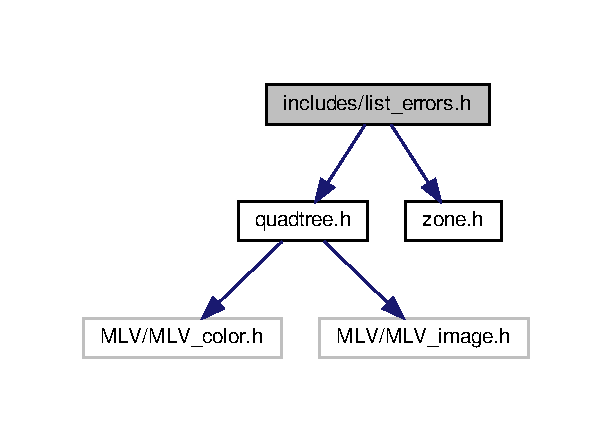
\includegraphics[width=294pt]{list__errors_8h__incl}
\end{center}
\end{figure}
This graph shows which files directly or indirectly include this file\+:
\nopagebreak
\begin{figure}[H]
\begin{center}
\leavevmode
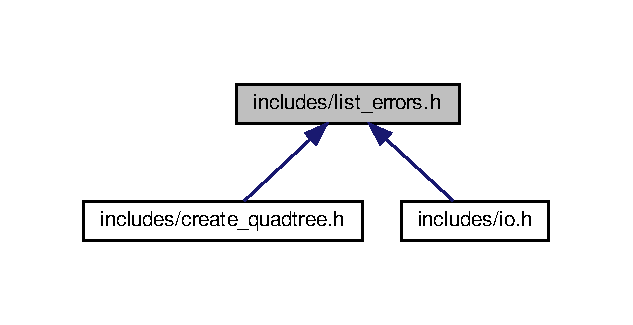
\includegraphics[width=304pt]{list__errors_8h__dep__incl}
\end{center}
\end{figure}
\subsection*{Data Structures}
\begin{DoxyCompactItemize}
\item 
struct \hyperlink{structErrorListElement}{Error\+List\+Element}
\item 
struct \hyperlink{structErrorList__FirstLast}{Error\+List\+\_\+\+First\+Last}
\end{DoxyCompactItemize}
\subsection*{Typedefs}
\begin{DoxyCompactItemize}
\item 
typedef struct \hyperlink{structErrorListElement}{Error\+List\+Element} \hyperlink{list__errors_8h_a73ff1284b66d1b6236711f2fec3c6162}{Error\+List\+Element}
\item 
typedef struct \hyperlink{structErrorListElement}{Error\+List\+Element} $\ast$ \hyperlink{list__errors_8h_a90522ae3e839b4beec367e58bc649808}{Error\+List}
\item 
typedef struct \hyperlink{structErrorList__FirstLast}{Error\+List\+\_\+\+First\+Last} \hyperlink{list__errors_8h_a4d2489819c47d5a1da95afa5935355b8}{Error\+List\+\_\+\+First\+Last}
\end{DoxyCompactItemize}
\subsection*{Functions}
\begin{DoxyCompactItemize}
\item 
void \hyperlink{list__errors_8h_a9436838d3661eac252baefd96ea699ce}{initialize\+\_\+firstlast} (\hyperlink{structErrorList__FirstLast}{Error\+List\+\_\+\+First\+Last} $\ast$list)
\begin{DoxyCompactList}\small\item\em Initialize an \hyperlink{structErrorList__FirstLast}{Error\+List\+\_\+\+First\+Last} (N\+U\+LL). \end{DoxyCompactList}\item 
void \hyperlink{list__errors_8h_a7b419c8705bffbbcad1690c4feefc534}{free\+\_\+error\+\_\+list} (\hyperlink{list__errors_8h_a90522ae3e839b4beec367e58bc649808}{Error\+List} $\ast$list)
\begin{DoxyCompactList}\small\item\em Free an \hyperlink{structErrorListElement}{Error\+List\+Element}. \end{DoxyCompactList}\item 
void \hyperlink{list__errors_8h_adebf1d95e3d18432ff40f3544c8d1b3d}{print\+\_\+error\+\_\+list} (\hyperlink{list__errors_8h_a90522ae3e839b4beec367e58bc649808}{Error\+List} $\ast$list)
\begin{DoxyCompactList}\small\item\em Print an \hyperlink{structErrorListElement}{Error\+List\+Element}. \end{DoxyCompactList}\item 
int \hyperlink{list__errors_8h_ab80a81c290a79257547d42a58778bcef}{add\+\_\+elem} (\hyperlink{list__errors_8h_a90522ae3e839b4beec367e58bc649808}{Error\+List} $\ast$list, \hyperlink{list__errors_8h_a90522ae3e839b4beec367e58bc649808}{Error\+List} $\ast$last, \hyperlink{quadtree_8h_a184f2f10109642ad84b5619bcc5738da}{Tree} $\ast$leaf, \hyperlink{structZone}{Zone} zone)
\begin{DoxyCompactList}\small\item\em Add an element in an Error\+List. \end{DoxyCompactList}\item 
int \hyperlink{list__errors_8h_a0525db8e99bf238ccbf42553361f22b1}{remove\+\_\+elem\+\_\+errorlist} (\hyperlink{list__errors_8h_a90522ae3e839b4beec367e58bc649808}{Error\+List} $\ast$list, double error)
\begin{DoxyCompactList}\small\item\em Remove an element from Error\+List by looking at its error value. \end{DoxyCompactList}\end{DoxyCompactItemize}


\subsection{Typedef Documentation}
\mbox{\Hypertarget{list__errors_8h_a90522ae3e839b4beec367e58bc649808}\label{list__errors_8h_a90522ae3e839b4beec367e58bc649808}} 
\index{list\+\_\+errors.\+h@{list\+\_\+errors.\+h}!Error\+List@{Error\+List}}
\index{Error\+List@{Error\+List}!list\+\_\+errors.\+h@{list\+\_\+errors.\+h}}
\subsubsection{\texorpdfstring{Error\+List}{ErrorList}}
{\footnotesize\ttfamily typedef struct \hyperlink{structErrorListElement}{Error\+List\+Element} $\ast$ \hyperlink{list__errors_8h_a90522ae3e839b4beec367e58bc649808}{Error\+List}}

\mbox{\Hypertarget{list__errors_8h_a4d2489819c47d5a1da95afa5935355b8}\label{list__errors_8h_a4d2489819c47d5a1da95afa5935355b8}} 
\index{list\+\_\+errors.\+h@{list\+\_\+errors.\+h}!Error\+List\+\_\+\+First\+Last@{Error\+List\+\_\+\+First\+Last}}
\index{Error\+List\+\_\+\+First\+Last@{Error\+List\+\_\+\+First\+Last}!list\+\_\+errors.\+h@{list\+\_\+errors.\+h}}
\subsubsection{\texorpdfstring{Error\+List\+\_\+\+First\+Last}{ErrorList\_FirstLast}}
{\footnotesize\ttfamily typedef struct \hyperlink{structErrorList__FirstLast}{Error\+List\+\_\+\+First\+Last}  \hyperlink{structErrorList__FirstLast}{Error\+List\+\_\+\+First\+Last}}

\mbox{\Hypertarget{list__errors_8h_a73ff1284b66d1b6236711f2fec3c6162}\label{list__errors_8h_a73ff1284b66d1b6236711f2fec3c6162}} 
\index{list\+\_\+errors.\+h@{list\+\_\+errors.\+h}!Error\+List\+Element@{Error\+List\+Element}}
\index{Error\+List\+Element@{Error\+List\+Element}!list\+\_\+errors.\+h@{list\+\_\+errors.\+h}}
\subsubsection{\texorpdfstring{Error\+List\+Element}{ErrorListElement}}
{\footnotesize\ttfamily typedef struct \hyperlink{structErrorListElement}{Error\+List\+Element}  \hyperlink{structErrorListElement}{Error\+List\+Element}}



\subsection{Function Documentation}
\mbox{\Hypertarget{list__errors_8h_ab80a81c290a79257547d42a58778bcef}\label{list__errors_8h_ab80a81c290a79257547d42a58778bcef}} 
\index{list\+\_\+errors.\+h@{list\+\_\+errors.\+h}!add\+\_\+elem@{add\+\_\+elem}}
\index{add\+\_\+elem@{add\+\_\+elem}!list\+\_\+errors.\+h@{list\+\_\+errors.\+h}}
\subsubsection{\texorpdfstring{add\+\_\+elem()}{add\_elem()}}
{\footnotesize\ttfamily int add\+\_\+elem (\begin{DoxyParamCaption}\item[{\hyperlink{list__errors_8h_a90522ae3e839b4beec367e58bc649808}{Error\+List} $\ast$}]{list,  }\item[{\hyperlink{list__errors_8h_a90522ae3e839b4beec367e58bc649808}{Error\+List} $\ast$}]{last,  }\item[{\hyperlink{quadtree_8h_a184f2f10109642ad84b5619bcc5738da}{Tree} $\ast$}]{leaf,  }\item[{\hyperlink{structZone}{Zone}}]{zone }\end{DoxyParamCaption})}



Add an element in an Error\+List. 


\begin{DoxyParams}{Parameters}
{\em list} & The list we are adding the element in \\
\hline
{\em last} & Pointer of last element of list \\
\hline
{\em leaf} & The leaf and its error we are adding \\
\hline
{\em zone} & Leaf\textquotesingle{}s zone in the image it\textquotesingle{}s coming from \\
\hline
\end{DoxyParams}
\begin{DoxyReturn}{Returns}
1 we add leaf\textquotesingle{}s and its error in list 0 otherwise (malloc pb) 
\end{DoxyReturn}
\mbox{\Hypertarget{list__errors_8h_a7b419c8705bffbbcad1690c4feefc534}\label{list__errors_8h_a7b419c8705bffbbcad1690c4feefc534}} 
\index{list\+\_\+errors.\+h@{list\+\_\+errors.\+h}!free\+\_\+error\+\_\+list@{free\+\_\+error\+\_\+list}}
\index{free\+\_\+error\+\_\+list@{free\+\_\+error\+\_\+list}!list\+\_\+errors.\+h@{list\+\_\+errors.\+h}}
\subsubsection{\texorpdfstring{free\+\_\+error\+\_\+list()}{free\_error\_list()}}
{\footnotesize\ttfamily void free\+\_\+error\+\_\+list (\begin{DoxyParamCaption}\item[{\hyperlink{list__errors_8h_a90522ae3e839b4beec367e58bc649808}{Error\+List} $\ast$}]{list }\end{DoxyParamCaption})}



Free an \hyperlink{structErrorListElement}{Error\+List\+Element}. 


\begin{DoxyParams}{Parameters}
{\em list} & The list we are freeing \\
\hline
\end{DoxyParams}
\mbox{\Hypertarget{list__errors_8h_a9436838d3661eac252baefd96ea699ce}\label{list__errors_8h_a9436838d3661eac252baefd96ea699ce}} 
\index{list\+\_\+errors.\+h@{list\+\_\+errors.\+h}!initialize\+\_\+firstlast@{initialize\+\_\+firstlast}}
\index{initialize\+\_\+firstlast@{initialize\+\_\+firstlast}!list\+\_\+errors.\+h@{list\+\_\+errors.\+h}}
\subsubsection{\texorpdfstring{initialize\+\_\+firstlast()}{initialize\_firstlast()}}
{\footnotesize\ttfamily void initialize\+\_\+firstlast (\begin{DoxyParamCaption}\item[{\hyperlink{structErrorList__FirstLast}{Error\+List\+\_\+\+First\+Last} $\ast$}]{list }\end{DoxyParamCaption})}



Initialize an \hyperlink{structErrorList__FirstLast}{Error\+List\+\_\+\+First\+Last} (N\+U\+LL). 


\begin{DoxyParams}{Parameters}
{\em list} & The \hyperlink{structErrorList__FirstLast}{Error\+List\+\_\+\+First\+Last} we are initializing \\
\hline
\end{DoxyParams}
\mbox{\Hypertarget{list__errors_8h_adebf1d95e3d18432ff40f3544c8d1b3d}\label{list__errors_8h_adebf1d95e3d18432ff40f3544c8d1b3d}} 
\index{list\+\_\+errors.\+h@{list\+\_\+errors.\+h}!print\+\_\+error\+\_\+list@{print\+\_\+error\+\_\+list}}
\index{print\+\_\+error\+\_\+list@{print\+\_\+error\+\_\+list}!list\+\_\+errors.\+h@{list\+\_\+errors.\+h}}
\subsubsection{\texorpdfstring{print\+\_\+error\+\_\+list()}{print\_error\_list()}}
{\footnotesize\ttfamily void print\+\_\+error\+\_\+list (\begin{DoxyParamCaption}\item[{\hyperlink{list__errors_8h_a90522ae3e839b4beec367e58bc649808}{Error\+List} $\ast$}]{list }\end{DoxyParamCaption})}



Print an \hyperlink{structErrorListElement}{Error\+List\+Element}. 


\begin{DoxyParams}{Parameters}
{\em list} & The list we are printing \\
\hline
\end{DoxyParams}
\mbox{\Hypertarget{list__errors_8h_a0525db8e99bf238ccbf42553361f22b1}\label{list__errors_8h_a0525db8e99bf238ccbf42553361f22b1}} 
\index{list\+\_\+errors.\+h@{list\+\_\+errors.\+h}!remove\+\_\+elem\+\_\+errorlist@{remove\+\_\+elem\+\_\+errorlist}}
\index{remove\+\_\+elem\+\_\+errorlist@{remove\+\_\+elem\+\_\+errorlist}!list\+\_\+errors.\+h@{list\+\_\+errors.\+h}}
\subsubsection{\texorpdfstring{remove\+\_\+elem\+\_\+errorlist()}{remove\_elem\_errorlist()}}
{\footnotesize\ttfamily int remove\+\_\+elem\+\_\+errorlist (\begin{DoxyParamCaption}\item[{\hyperlink{list__errors_8h_a90522ae3e839b4beec367e58bc649808}{Error\+List} $\ast$}]{list,  }\item[{double}]{error }\end{DoxyParamCaption})}



Remove an element from Error\+List by looking at its error value. 


\begin{DoxyParams}{Parameters}
{\em list} & explication \\
\hline
\end{DoxyParams}
\begin{DoxyReturn}{Returns}
-\/2 if we couldn\textquotesingle{}t find the error value -\/1 if list is empty 0 if we removed an element 
\end{DoxyReturn}

\hypertarget{minimisation_8h}{}\section{includes/minimisation.h File Reference}
\label{minimisation_8h}\index{includes/minimisation.\+h@{includes/minimisation.\+h}}
{\ttfamily \#include \char`\"{}color.\+h\char`\"{}}\newline
{\ttfamily \#include \char`\"{}quadtree.\+h\char`\"{}}\newline
{\ttfamily \#include \char`\"{}zone.\+h\char`\"{}}\newline
Include dependency graph for minimisation.\+h\+:
\nopagebreak
\begin{figure}[H]
\begin{center}
\leavevmode
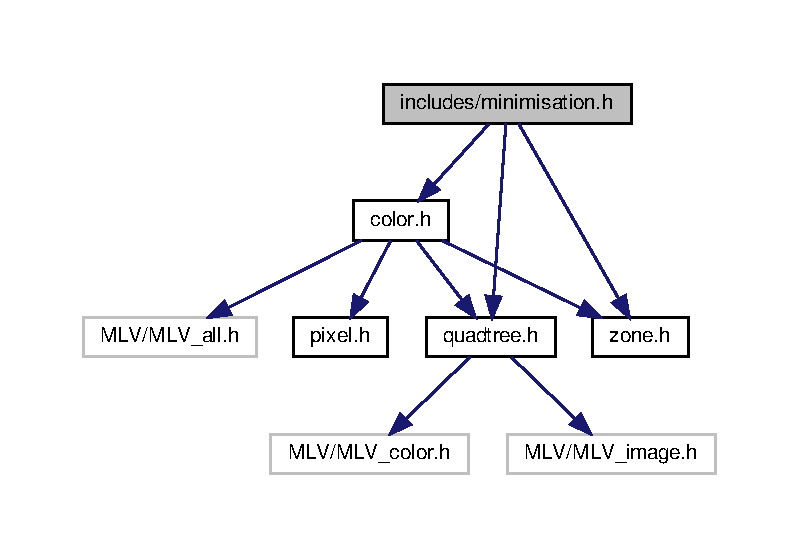
\includegraphics[width=350pt]{minimisation_8h__incl}
\end{center}
\end{figure}
\subsection*{Macros}
\begin{DoxyCompactItemize}
\item 
\#define \hyperlink{minimisation_8h_ad1f7f78b7e7843ca8a2f94fcc8482ceb}{D\+I\+S\+T\+\_\+\+M\+AX}~7.\+5
\item 
\#define \hyperlink{minimisation_8h_af858ce84831caa5b5daaf9d9776ca547}{E\+R\+R\+O\+R\+\_\+\+M\+AX}~100.\+0
\end{DoxyCompactItemize}
\subsection*{Functions}
\begin{DoxyCompactItemize}
\item 
void \hyperlink{minimisation_8h_aef0439c213cf617f1f2559f6cd6a425e}{minimize\+\_\+without\+\_\+loss} (\hyperlink{quadtree_8h_a184f2f10109642ad84b5619bcc5738da}{Tree} $\ast$$\ast$t)
\begin{DoxyCompactList}\small\item\em Minimize a tree without loss \+: if a node with a heigh of 1 still have all of its leaf with the same color, we replace the leaf with one of its leaf. \end{DoxyCompactList}\item 
void \hyperlink{minimisation_8h_a123478c12f569d3e6276af27e0ad2310}{minimize\+\_\+loss} (\hyperlink{quadtree_8h_a184f2f10109642ad84b5619bcc5738da}{Tree} $\ast$$\ast$t, const M\+L\+V\+\_\+\+Image $\ast$image, \hyperlink{structZone}{Zone} zone)
\begin{DoxyCompactList}\small\item\em Minimize a tree with loss \+: minimize a quadtree using both minimize\+\_\+loss\+\_\+remove\+\_\+small\+\_\+errors and minimize\+\_\+loss\+\_\+fuse\+\_\+identical\+\_\+subtree functions. \end{DoxyCompactList}\end{DoxyCompactItemize}


\subsection{Macro Definition Documentation}
\mbox{\Hypertarget{minimisation_8h_ad1f7f78b7e7843ca8a2f94fcc8482ceb}\label{minimisation_8h_ad1f7f78b7e7843ca8a2f94fcc8482ceb}} 
\index{minimisation.\+h@{minimisation.\+h}!D\+I\+S\+T\+\_\+\+M\+AX@{D\+I\+S\+T\+\_\+\+M\+AX}}
\index{D\+I\+S\+T\+\_\+\+M\+AX@{D\+I\+S\+T\+\_\+\+M\+AX}!minimisation.\+h@{minimisation.\+h}}
\subsubsection{\texorpdfstring{D\+I\+S\+T\+\_\+\+M\+AX}{DIST\_MAX}}
{\footnotesize\ttfamily \#define D\+I\+S\+T\+\_\+\+M\+AX~7.\+5}

\mbox{\Hypertarget{minimisation_8h_af858ce84831caa5b5daaf9d9776ca547}\label{minimisation_8h_af858ce84831caa5b5daaf9d9776ca547}} 
\index{minimisation.\+h@{minimisation.\+h}!E\+R\+R\+O\+R\+\_\+\+M\+AX@{E\+R\+R\+O\+R\+\_\+\+M\+AX}}
\index{E\+R\+R\+O\+R\+\_\+\+M\+AX@{E\+R\+R\+O\+R\+\_\+\+M\+AX}!minimisation.\+h@{minimisation.\+h}}
\subsubsection{\texorpdfstring{E\+R\+R\+O\+R\+\_\+\+M\+AX}{ERROR\_MAX}}
{\footnotesize\ttfamily \#define E\+R\+R\+O\+R\+\_\+\+M\+AX~100.\+0}



\subsection{Function Documentation}
\mbox{\Hypertarget{minimisation_8h_a123478c12f569d3e6276af27e0ad2310}\label{minimisation_8h_a123478c12f569d3e6276af27e0ad2310}} 
\index{minimisation.\+h@{minimisation.\+h}!minimize\+\_\+loss@{minimize\+\_\+loss}}
\index{minimize\+\_\+loss@{minimize\+\_\+loss}!minimisation.\+h@{minimisation.\+h}}
\subsubsection{\texorpdfstring{minimize\+\_\+loss()}{minimize\_loss()}}
{\footnotesize\ttfamily void minimize\+\_\+loss (\begin{DoxyParamCaption}\item[{\hyperlink{quadtree_8h_a184f2f10109642ad84b5619bcc5738da}{Tree} $\ast$$\ast$}]{t,  }\item[{const M\+L\+V\+\_\+\+Image $\ast$}]{image,  }\item[{\hyperlink{structZone}{Zone}}]{zone }\end{DoxyParamCaption})}



Minimize a tree with loss \+: minimize a quadtree using both minimize\+\_\+loss\+\_\+remove\+\_\+small\+\_\+errors and minimize\+\_\+loss\+\_\+fuse\+\_\+identical\+\_\+subtree functions. 


\begin{DoxyParams}{Parameters}
{\em t} & The tree we are minimizing \\
\hline
{\em image} & The image the tree is created from \\
\hline
{\em zone} & The zone we are minimizing \\
\hline
\end{DoxyParams}
\mbox{\Hypertarget{minimisation_8h_aef0439c213cf617f1f2559f6cd6a425e}\label{minimisation_8h_aef0439c213cf617f1f2559f6cd6a425e}} 
\index{minimisation.\+h@{minimisation.\+h}!minimize\+\_\+without\+\_\+loss@{minimize\+\_\+without\+\_\+loss}}
\index{minimize\+\_\+without\+\_\+loss@{minimize\+\_\+without\+\_\+loss}!minimisation.\+h@{minimisation.\+h}}
\subsubsection{\texorpdfstring{minimize\+\_\+without\+\_\+loss()}{minimize\_without\_loss()}}
{\footnotesize\ttfamily void minimize\+\_\+without\+\_\+loss (\begin{DoxyParamCaption}\item[{\hyperlink{quadtree_8h_a184f2f10109642ad84b5619bcc5738da}{Tree} $\ast$$\ast$}]{t }\end{DoxyParamCaption})}



Minimize a tree without loss \+: if a node with a heigh of 1 still have all of its leaf with the same color, we replace the leaf with one of its leaf. 


\begin{DoxyParams}{Parameters}
{\em t} & The tree we are minimizing \\
\hline
\end{DoxyParams}

\hypertarget{pixel_8h}{}\section{includes/pixel.h File Reference}
\label{pixel_8h}\index{includes/pixel.\+h@{includes/pixel.\+h}}
This graph shows which files directly or indirectly include this file\+:
\nopagebreak
\begin{figure}[H]
\begin{center}
\leavevmode
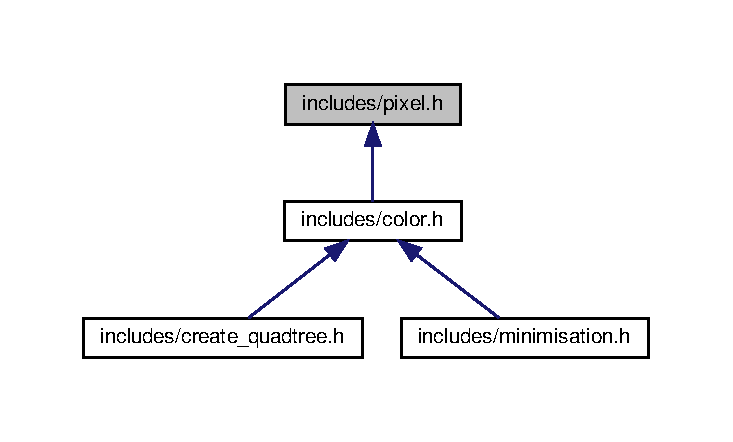
\includegraphics[width=350pt]{pixel_8h__dep__incl}
\end{center}
\end{figure}
\subsection*{Data Structures}
\begin{DoxyCompactItemize}
\item 
struct \hyperlink{structPixel}{Pixel}
\end{DoxyCompactItemize}
\subsection*{Functions}
\begin{DoxyCompactItemize}
\item 
double \hyperlink{pixel_8h_aaafeb482146acf212e12a67a728316da}{pixel\+\_\+distance} (\hyperlink{structPixel}{Pixel} p1, \hyperlink{structPixel}{Pixel} p2)
\begin{DoxyCompactList}\small\item\em Returns the distance between 2 pixels in rgba. \end{DoxyCompactList}\end{DoxyCompactItemize}


\subsection{Function Documentation}
\mbox{\Hypertarget{pixel_8h_aaafeb482146acf212e12a67a728316da}\label{pixel_8h_aaafeb482146acf212e12a67a728316da}} 
\index{pixel.\+h@{pixel.\+h}!pixel\+\_\+distance@{pixel\+\_\+distance}}
\index{pixel\+\_\+distance@{pixel\+\_\+distance}!pixel.\+h@{pixel.\+h}}
\subsubsection{\texorpdfstring{pixel\+\_\+distance()}{pixel\_distance()}}
{\footnotesize\ttfamily double pixel\+\_\+distance (\begin{DoxyParamCaption}\item[{\hyperlink{structPixel}{Pixel}}]{p1,  }\item[{\hyperlink{structPixel}{Pixel}}]{p2 }\end{DoxyParamCaption})}



Returns the distance between 2 pixels in rgba. 


\begin{DoxyParams}{Parameters}
{\em p1} & The first pixel \\
\hline
{\em p2} & The second pixel \\
\hline
\end{DoxyParams}
\begin{DoxyReturn}{Returns}
Distance between p1 and p2 
\end{DoxyReturn}

\hypertarget{quadtree_8h}{}\section{includes/quadtree.h File Reference}
\label{quadtree_8h}\index{includes/quadtree.\+h@{includes/quadtree.\+h}}
{\ttfamily \#include $<$M\+L\+V/\+M\+L\+V\+\_\+color.\+h$>$}\newline
{\ttfamily \#include $<$M\+L\+V/\+M\+L\+V\+\_\+image.\+h$>$}\newline
Include dependency graph for quadtree.\+h\+:
\nopagebreak
\begin{figure}[H]
\begin{center}
\leavevmode
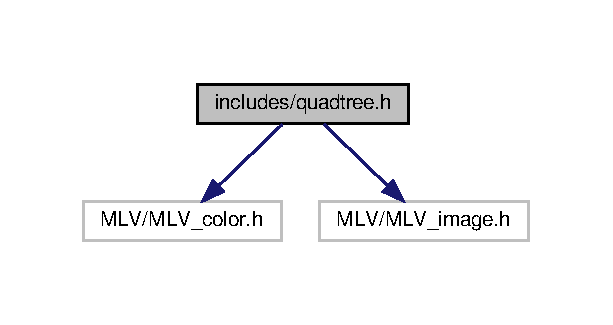
\includegraphics[width=294pt]{quadtree_8h__incl}
\end{center}
\end{figure}
This graph shows which files directly or indirectly include this file\+:
\nopagebreak
\begin{figure}[H]
\begin{center}
\leavevmode
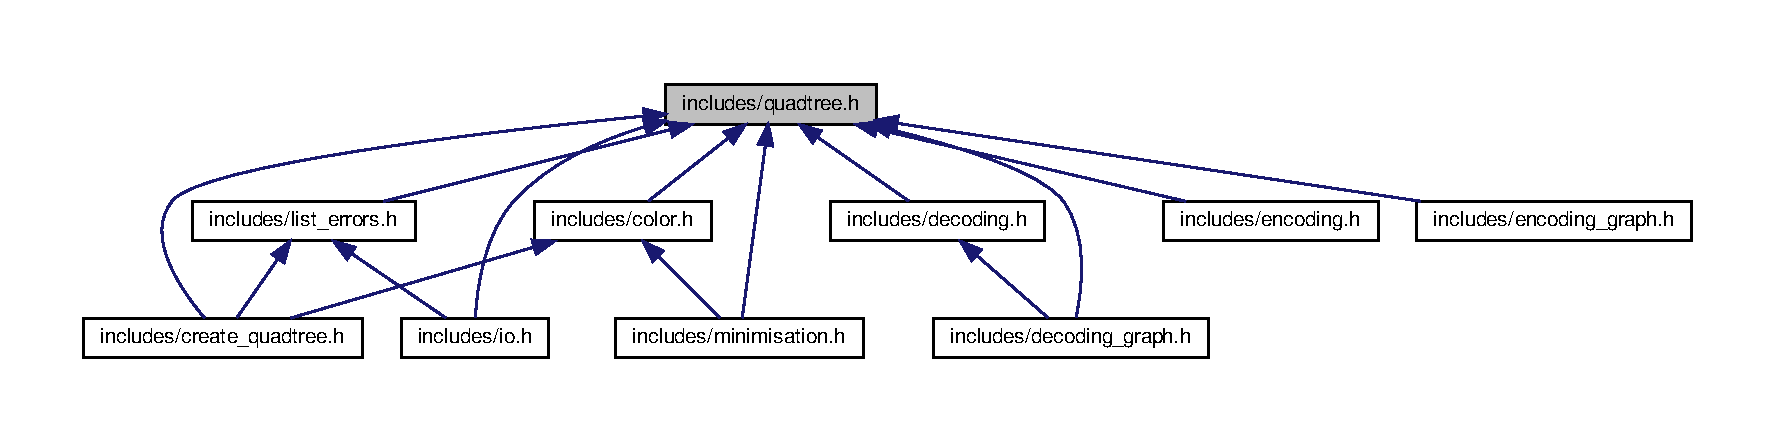
\includegraphics[width=350pt]{quadtree_8h__dep__incl}
\end{center}
\end{figure}
\subsection*{Data Structures}
\begin{DoxyCompactItemize}
\item 
union \hyperlink{unionSub__tree}{Sub\+\_\+tree}
\item 
struct \hyperlink{structquad}{quad}
\end{DoxyCompactItemize}
\subsection*{Macros}
\begin{DoxyCompactItemize}
\item 
\#define \hyperlink{quadtree_8h_a07c883b063ae8a373a3c9b5356f5fa8d}{S\+I\+Z\+E\+\_\+\+I\+M\+A\+GE}~512
\item 
\#define \hyperlink{quadtree_8h_ad4064b9a55688d57356121bd89f34fd0}{N\+B\+\_\+\+S\+H\+A\+R\+ES}~131072
\end{DoxyCompactItemize}
\subsection*{Typedefs}
\begin{DoxyCompactItemize}
\item 
typedef struct \hyperlink{structquad}{quad} \hyperlink{quadtree_8h_a184f2f10109642ad84b5619bcc5738da}{Tree}
\end{DoxyCompactItemize}
\subsection*{Enumerations}
\begin{DoxyCompactItemize}
\item 
enum \hyperlink{quadtree_8h_a4bafb4a83e1da39fd7547ca43cff608d}{Node\+\_\+type} \{ \hyperlink{quadtree_8h_a4bafb4a83e1da39fd7547ca43cff608da150d9833918207030adb030ccc759c20}{L\+E\+AF}, 
\hyperlink{quadtree_8h_a4bafb4a83e1da39fd7547ca43cff608da59a889456a2d742fdca191dccb3e871d}{N\+O\+DE}
 \}
\item 
enum \hyperlink{quadtree_8h_a54cad6fa8fbf6a3b3083585da4a26731}{Kid\+\_\+type} \{ \hyperlink{quadtree_8h_a54cad6fa8fbf6a3b3083585da4a26731a0d077f5b932ce05e5b9f30c6087a2f31}{NO}, 
\hyperlink{quadtree_8h_a54cad6fa8fbf6a3b3083585da4a26731a4d3f872f5054b256b01ee4f2c8cf51db}{NE}, 
\hyperlink{quadtree_8h_a54cad6fa8fbf6a3b3083585da4a26731af9f590fe6d84e72c832e714b75b1604b}{SO}, 
\hyperlink{quadtree_8h_a54cad6fa8fbf6a3b3083585da4a26731a61c600c17d14bd4db73433ddbb8491e8}{SE}
 \}
\end{DoxyCompactItemize}
\subsection*{Functions}
\begin{DoxyCompactItemize}
\item 
int \hyperlink{quadtree_8h_ac27735a0294f989007ba6509f74914f4}{is\+\_\+leaf} (\hyperlink{quadtree_8h_a184f2f10109642ad84b5619bcc5738da}{Tree} $\ast$t)
\begin{DoxyCompactList}\small\item\em Check if \char`\"{}t\char`\"{} is a leaf. \end{DoxyCompactList}\item 
int \hyperlink{quadtree_8h_a501cabb1f7635abf0660b5fe7a5a8b78}{is\+\_\+node} (\hyperlink{quadtree_8h_a184f2f10109642ad84b5619bcc5738da}{Tree} $\ast$t)
\begin{DoxyCompactList}\small\item\em Check if \char`\"{}t\char`\"{} is a node. \end{DoxyCompactList}\item 
int \hyperlink{quadtree_8h_aa93410d380db7cec4675f69eb188e97c}{has\+\_\+full\+\_\+leaf} (\hyperlink{quadtree_8h_a184f2f10109642ad84b5619bcc5738da}{Tree} $\ast$t)
\begin{DoxyCompactList}\small\item\em Check if \char`\"{}t\char`\"{} is a node, and if NO, NE, SE and SO are leaf. \end{DoxyCompactList}\item 
void \hyperlink{quadtree_8h_a7ee52185703e339f9b37a0e84eba57f8}{print\+\_\+tree\+\_\+prefix} (\hyperlink{quadtree_8h_a184f2f10109642ad84b5619bcc5738da}{Tree} $\ast$t)
\begin{DoxyCompactList}\small\item\em Print a tree in prefix order. \end{DoxyCompactList}\item 
void \hyperlink{quadtree_8h_a2d53b82f6524522d0ea84d28c9b9355a}{print\+\_\+node} (\hyperlink{quadtree_8h_a184f2f10109642ad84b5619bcc5738da}{Tree} $\ast$t)
\begin{DoxyCompactList}\small\item\em Print a node. \end{DoxyCompactList}\item 
void \hyperlink{quadtree_8h_acbc1cb9bce582ea945e4a467c76a57aa}{free\+\_\+tree} (\hyperlink{quadtree_8h_a184f2f10109642ad84b5619bcc5738da}{Tree} $\ast$t)
\begin{DoxyCompactList}\small\item\em Free a tree. \end{DoxyCompactList}\item 
void \hyperlink{quadtree_8h_ac566469b25896389b3c9d4098b42d61a}{free\+\_\+all\+\_\+leaf} (\hyperlink{quadtree_8h_a184f2f10109642ad84b5619bcc5738da}{Tree} $\ast$t)
\begin{DoxyCompactList}\small\item\em Free all t\textquotesingle{}s leaf. \end{DoxyCompactList}\item 
void \hyperlink{quadtree_8h_a02d9ec6b7a28a38105be2476c5665410}{replace\+\_\+node\+\_\+to\+\_\+leaf} (\hyperlink{quadtree_8h_a184f2f10109642ad84b5619bcc5738da}{Tree} $\ast$$\ast$node, \hyperlink{quadtree_8h_a184f2f10109642ad84b5619bcc5738da}{Tree} $\ast$leaf)
\begin{DoxyCompactList}\small\item\em Replace a node with a leaf. \end{DoxyCompactList}\item 
int \hyperlink{quadtree_8h_a7cc2fcae342be657d1cf8d848fd4ecce}{tree\+\_\+to\+\_\+image} (M\+L\+V\+\_\+\+Image $\ast$$\ast$img, \hyperlink{quadtree_8h_a184f2f10109642ad84b5619bcc5738da}{Tree} $\ast$t)
\begin{DoxyCompactList}\small\item\em Fill an image with a subtree. \end{DoxyCompactList}\end{DoxyCompactItemize}


\subsection{Macro Definition Documentation}
\mbox{\Hypertarget{quadtree_8h_ad4064b9a55688d57356121bd89f34fd0}\label{quadtree_8h_ad4064b9a55688d57356121bd89f34fd0}} 
\index{quadtree.\+h@{quadtree.\+h}!N\+B\+\_\+\+S\+H\+A\+R\+ES@{N\+B\+\_\+\+S\+H\+A\+R\+ES}}
\index{N\+B\+\_\+\+S\+H\+A\+R\+ES@{N\+B\+\_\+\+S\+H\+A\+R\+ES}!quadtree.\+h@{quadtree.\+h}}
\subsubsection{\texorpdfstring{N\+B\+\_\+\+S\+H\+A\+R\+ES}{NB\_SHARES}}
{\footnotesize\ttfamily \#define N\+B\+\_\+\+S\+H\+A\+R\+ES~131072}

\mbox{\Hypertarget{quadtree_8h_a07c883b063ae8a373a3c9b5356f5fa8d}\label{quadtree_8h_a07c883b063ae8a373a3c9b5356f5fa8d}} 
\index{quadtree.\+h@{quadtree.\+h}!S\+I\+Z\+E\+\_\+\+I\+M\+A\+GE@{S\+I\+Z\+E\+\_\+\+I\+M\+A\+GE}}
\index{S\+I\+Z\+E\+\_\+\+I\+M\+A\+GE@{S\+I\+Z\+E\+\_\+\+I\+M\+A\+GE}!quadtree.\+h@{quadtree.\+h}}
\subsubsection{\texorpdfstring{S\+I\+Z\+E\+\_\+\+I\+M\+A\+GE}{SIZE\_IMAGE}}
{\footnotesize\ttfamily \#define S\+I\+Z\+E\+\_\+\+I\+M\+A\+GE~512}



\subsection{Typedef Documentation}
\mbox{\Hypertarget{quadtree_8h_a184f2f10109642ad84b5619bcc5738da}\label{quadtree_8h_a184f2f10109642ad84b5619bcc5738da}} 
\index{quadtree.\+h@{quadtree.\+h}!Tree@{Tree}}
\index{Tree@{Tree}!quadtree.\+h@{quadtree.\+h}}
\subsubsection{\texorpdfstring{Tree}{Tree}}
{\footnotesize\ttfamily typedef struct \hyperlink{structquad}{quad}  \hyperlink{quadtree_8h_a184f2f10109642ad84b5619bcc5738da}{Tree}}



\subsection{Enumeration Type Documentation}
\mbox{\Hypertarget{quadtree_8h_a54cad6fa8fbf6a3b3083585da4a26731}\label{quadtree_8h_a54cad6fa8fbf6a3b3083585da4a26731}} 
\index{quadtree.\+h@{quadtree.\+h}!Kid\+\_\+type@{Kid\+\_\+type}}
\index{Kid\+\_\+type@{Kid\+\_\+type}!quadtree.\+h@{quadtree.\+h}}
\subsubsection{\texorpdfstring{Kid\+\_\+type}{Kid\_type}}
{\footnotesize\ttfamily enum \hyperlink{quadtree_8h_a54cad6fa8fbf6a3b3083585da4a26731}{Kid\+\_\+type}}

\begin{DoxyEnumFields}{Enumerator}
\raisebox{\heightof{T}}[0pt][0pt]{\index{NO@{NO}!quadtree.\+h@{quadtree.\+h}}\index{quadtree.\+h@{quadtree.\+h}!NO@{NO}}}\mbox{\Hypertarget{quadtree_8h_a54cad6fa8fbf6a3b3083585da4a26731a0d077f5b932ce05e5b9f30c6087a2f31}\label{quadtree_8h_a54cad6fa8fbf6a3b3083585da4a26731a0d077f5b932ce05e5b9f30c6087a2f31}} 
NO&\\
\hline

\raisebox{\heightof{T}}[0pt][0pt]{\index{NE@{NE}!quadtree.\+h@{quadtree.\+h}}\index{quadtree.\+h@{quadtree.\+h}!NE@{NE}}}\mbox{\Hypertarget{quadtree_8h_a54cad6fa8fbf6a3b3083585da4a26731a4d3f872f5054b256b01ee4f2c8cf51db}\label{quadtree_8h_a54cad6fa8fbf6a3b3083585da4a26731a4d3f872f5054b256b01ee4f2c8cf51db}} 
NE&\\
\hline

\raisebox{\heightof{T}}[0pt][0pt]{\index{SO@{SO}!quadtree.\+h@{quadtree.\+h}}\index{quadtree.\+h@{quadtree.\+h}!SO@{SO}}}\mbox{\Hypertarget{quadtree_8h_a54cad6fa8fbf6a3b3083585da4a26731af9f590fe6d84e72c832e714b75b1604b}\label{quadtree_8h_a54cad6fa8fbf6a3b3083585da4a26731af9f590fe6d84e72c832e714b75b1604b}} 
SO&\\
\hline

\raisebox{\heightof{T}}[0pt][0pt]{\index{SE@{SE}!quadtree.\+h@{quadtree.\+h}}\index{quadtree.\+h@{quadtree.\+h}!SE@{SE}}}\mbox{\Hypertarget{quadtree_8h_a54cad6fa8fbf6a3b3083585da4a26731a61c600c17d14bd4db73433ddbb8491e8}\label{quadtree_8h_a54cad6fa8fbf6a3b3083585da4a26731a61c600c17d14bd4db73433ddbb8491e8}} 
SE&\\
\hline

\end{DoxyEnumFields}
\mbox{\Hypertarget{quadtree_8h_a4bafb4a83e1da39fd7547ca43cff608d}\label{quadtree_8h_a4bafb4a83e1da39fd7547ca43cff608d}} 
\index{quadtree.\+h@{quadtree.\+h}!Node\+\_\+type@{Node\+\_\+type}}
\index{Node\+\_\+type@{Node\+\_\+type}!quadtree.\+h@{quadtree.\+h}}
\subsubsection{\texorpdfstring{Node\+\_\+type}{Node\_type}}
{\footnotesize\ttfamily enum \hyperlink{quadtree_8h_a4bafb4a83e1da39fd7547ca43cff608d}{Node\+\_\+type}}

\begin{DoxyEnumFields}{Enumerator}
\raisebox{\heightof{T}}[0pt][0pt]{\index{L\+E\+AF@{L\+E\+AF}!quadtree.\+h@{quadtree.\+h}}\index{quadtree.\+h@{quadtree.\+h}!L\+E\+AF@{L\+E\+AF}}}\mbox{\Hypertarget{quadtree_8h_a4bafb4a83e1da39fd7547ca43cff608da150d9833918207030adb030ccc759c20}\label{quadtree_8h_a4bafb4a83e1da39fd7547ca43cff608da150d9833918207030adb030ccc759c20}} 
L\+E\+AF&\\
\hline

\raisebox{\heightof{T}}[0pt][0pt]{\index{N\+O\+DE@{N\+O\+DE}!quadtree.\+h@{quadtree.\+h}}\index{quadtree.\+h@{quadtree.\+h}!N\+O\+DE@{N\+O\+DE}}}\mbox{\Hypertarget{quadtree_8h_a4bafb4a83e1da39fd7547ca43cff608da59a889456a2d742fdca191dccb3e871d}\label{quadtree_8h_a4bafb4a83e1da39fd7547ca43cff608da59a889456a2d742fdca191dccb3e871d}} 
N\+O\+DE&\\
\hline

\end{DoxyEnumFields}


\subsection{Function Documentation}
\mbox{\Hypertarget{quadtree_8h_ac566469b25896389b3c9d4098b42d61a}\label{quadtree_8h_ac566469b25896389b3c9d4098b42d61a}} 
\index{quadtree.\+h@{quadtree.\+h}!free\+\_\+all\+\_\+leaf@{free\+\_\+all\+\_\+leaf}}
\index{free\+\_\+all\+\_\+leaf@{free\+\_\+all\+\_\+leaf}!quadtree.\+h@{quadtree.\+h}}
\subsubsection{\texorpdfstring{free\+\_\+all\+\_\+leaf()}{free\_all\_leaf()}}
{\footnotesize\ttfamily void free\+\_\+all\+\_\+leaf (\begin{DoxyParamCaption}\item[{\hyperlink{quadtree_8h_a184f2f10109642ad84b5619bcc5738da}{Tree} $\ast$}]{t }\end{DoxyParamCaption})}



Free all t\textquotesingle{}s leaf. 


\begin{DoxyParams}{Parameters}
{\em t} & The tree we\textquotesingle{}ll free \\
\hline
\end{DoxyParams}
\mbox{\Hypertarget{quadtree_8h_acbc1cb9bce582ea945e4a467c76a57aa}\label{quadtree_8h_acbc1cb9bce582ea945e4a467c76a57aa}} 
\index{quadtree.\+h@{quadtree.\+h}!free\+\_\+tree@{free\+\_\+tree}}
\index{free\+\_\+tree@{free\+\_\+tree}!quadtree.\+h@{quadtree.\+h}}
\subsubsection{\texorpdfstring{free\+\_\+tree()}{free\_tree()}}
{\footnotesize\ttfamily void free\+\_\+tree (\begin{DoxyParamCaption}\item[{\hyperlink{quadtree_8h_a184f2f10109642ad84b5619bcc5738da}{Tree} $\ast$}]{t }\end{DoxyParamCaption})}



Free a tree. 


\begin{DoxyParams}{Parameters}
{\em t} & The tree we\textquotesingle{}ll free \\
\hline
\end{DoxyParams}
\mbox{\Hypertarget{quadtree_8h_aa93410d380db7cec4675f69eb188e97c}\label{quadtree_8h_aa93410d380db7cec4675f69eb188e97c}} 
\index{quadtree.\+h@{quadtree.\+h}!has\+\_\+full\+\_\+leaf@{has\+\_\+full\+\_\+leaf}}
\index{has\+\_\+full\+\_\+leaf@{has\+\_\+full\+\_\+leaf}!quadtree.\+h@{quadtree.\+h}}
\subsubsection{\texorpdfstring{has\+\_\+full\+\_\+leaf()}{has\_full\_leaf()}}
{\footnotesize\ttfamily int has\+\_\+full\+\_\+leaf (\begin{DoxyParamCaption}\item[{\hyperlink{quadtree_8h_a184f2f10109642ad84b5619bcc5738da}{Tree} $\ast$}]{t }\end{DoxyParamCaption})}



Check if \char`\"{}t\char`\"{} is a node, and if NO, NE, SE and SO are leaf. 


\begin{DoxyParams}{Parameters}
{\em t} & The tree we are looking at \\
\hline
\end{DoxyParams}
\begin{DoxyReturn}{Returns}
1 if \char`\"{}t\char`\"{} is a node with only leafs 0 otherwise 
\end{DoxyReturn}
\mbox{\Hypertarget{quadtree_8h_ac27735a0294f989007ba6509f74914f4}\label{quadtree_8h_ac27735a0294f989007ba6509f74914f4}} 
\index{quadtree.\+h@{quadtree.\+h}!is\+\_\+leaf@{is\+\_\+leaf}}
\index{is\+\_\+leaf@{is\+\_\+leaf}!quadtree.\+h@{quadtree.\+h}}
\subsubsection{\texorpdfstring{is\+\_\+leaf()}{is\_leaf()}}
{\footnotesize\ttfamily int is\+\_\+leaf (\begin{DoxyParamCaption}\item[{\hyperlink{quadtree_8h_a184f2f10109642ad84b5619bcc5738da}{Tree} $\ast$}]{t }\end{DoxyParamCaption})}



Check if \char`\"{}t\char`\"{} is a leaf. 


\begin{DoxyParams}{Parameters}
{\em t} & The tree we are looking at \\
\hline
\end{DoxyParams}
\begin{DoxyReturn}{Returns}
1 if \char`\"{}t\char`\"{} is a leaf 0 otherwise 
\end{DoxyReturn}
\mbox{\Hypertarget{quadtree_8h_a501cabb1f7635abf0660b5fe7a5a8b78}\label{quadtree_8h_a501cabb1f7635abf0660b5fe7a5a8b78}} 
\index{quadtree.\+h@{quadtree.\+h}!is\+\_\+node@{is\+\_\+node}}
\index{is\+\_\+node@{is\+\_\+node}!quadtree.\+h@{quadtree.\+h}}
\subsubsection{\texorpdfstring{is\+\_\+node()}{is\_node()}}
{\footnotesize\ttfamily int is\+\_\+node (\begin{DoxyParamCaption}\item[{\hyperlink{quadtree_8h_a184f2f10109642ad84b5619bcc5738da}{Tree} $\ast$}]{t }\end{DoxyParamCaption})}



Check if \char`\"{}t\char`\"{} is a node. 


\begin{DoxyParams}{Parameters}
{\em t} & The tree we are looking at \\
\hline
\end{DoxyParams}
\begin{DoxyReturn}{Returns}
1 if \char`\"{}t\char`\"{} is a node 0 otherwise 
\end{DoxyReturn}
\mbox{\Hypertarget{quadtree_8h_a2d53b82f6524522d0ea84d28c9b9355a}\label{quadtree_8h_a2d53b82f6524522d0ea84d28c9b9355a}} 
\index{quadtree.\+h@{quadtree.\+h}!print\+\_\+node@{print\+\_\+node}}
\index{print\+\_\+node@{print\+\_\+node}!quadtree.\+h@{quadtree.\+h}}
\subsubsection{\texorpdfstring{print\+\_\+node()}{print\_node()}}
{\footnotesize\ttfamily void print\+\_\+node (\begin{DoxyParamCaption}\item[{\hyperlink{quadtree_8h_a184f2f10109642ad84b5619bcc5738da}{Tree} $\ast$}]{t }\end{DoxyParamCaption})}



Print a node. 


\begin{DoxyParams}{Parameters}
{\em t} & The node we\textquotesingle{}ll print \\
\hline
\end{DoxyParams}
\mbox{\Hypertarget{quadtree_8h_a7ee52185703e339f9b37a0e84eba57f8}\label{quadtree_8h_a7ee52185703e339f9b37a0e84eba57f8}} 
\index{quadtree.\+h@{quadtree.\+h}!print\+\_\+tree\+\_\+prefix@{print\+\_\+tree\+\_\+prefix}}
\index{print\+\_\+tree\+\_\+prefix@{print\+\_\+tree\+\_\+prefix}!quadtree.\+h@{quadtree.\+h}}
\subsubsection{\texorpdfstring{print\+\_\+tree\+\_\+prefix()}{print\_tree\_prefix()}}
{\footnotesize\ttfamily void print\+\_\+tree\+\_\+prefix (\begin{DoxyParamCaption}\item[{\hyperlink{quadtree_8h_a184f2f10109642ad84b5619bcc5738da}{Tree} $\ast$}]{t }\end{DoxyParamCaption})}



Print a tree in prefix order. 


\begin{DoxyParams}{Parameters}
{\em t} & The tree we\textquotesingle{}ll print \\
\hline
\end{DoxyParams}
\mbox{\Hypertarget{quadtree_8h_a02d9ec6b7a28a38105be2476c5665410}\label{quadtree_8h_a02d9ec6b7a28a38105be2476c5665410}} 
\index{quadtree.\+h@{quadtree.\+h}!replace\+\_\+node\+\_\+to\+\_\+leaf@{replace\+\_\+node\+\_\+to\+\_\+leaf}}
\index{replace\+\_\+node\+\_\+to\+\_\+leaf@{replace\+\_\+node\+\_\+to\+\_\+leaf}!quadtree.\+h@{quadtree.\+h}}
\subsubsection{\texorpdfstring{replace\+\_\+node\+\_\+to\+\_\+leaf()}{replace\_node\_to\_leaf()}}
{\footnotesize\ttfamily void replace\+\_\+node\+\_\+to\+\_\+leaf (\begin{DoxyParamCaption}\item[{\hyperlink{quadtree_8h_a184f2f10109642ad84b5619bcc5738da}{Tree} $\ast$$\ast$}]{node,  }\item[{\hyperlink{quadtree_8h_a184f2f10109642ad84b5619bcc5738da}{Tree} $\ast$}]{leaf }\end{DoxyParamCaption})}



Replace a node with a leaf. 


\begin{DoxyParams}{Parameters}
{\em node} & The node we replace \\
\hline
{\em leaf} & The leaf we take the fields from \\
\hline
\end{DoxyParams}
\mbox{\Hypertarget{quadtree_8h_a7cc2fcae342be657d1cf8d848fd4ecce}\label{quadtree_8h_a7cc2fcae342be657d1cf8d848fd4ecce}} 
\index{quadtree.\+h@{quadtree.\+h}!tree\+\_\+to\+\_\+image@{tree\+\_\+to\+\_\+image}}
\index{tree\+\_\+to\+\_\+image@{tree\+\_\+to\+\_\+image}!quadtree.\+h@{quadtree.\+h}}
\subsubsection{\texorpdfstring{tree\+\_\+to\+\_\+image()}{tree\_to\_image()}}
{\footnotesize\ttfamily int tree\+\_\+to\+\_\+image (\begin{DoxyParamCaption}\item[{M\+L\+V\+\_\+\+Image $\ast$$\ast$}]{img,  }\item[{\hyperlink{quadtree_8h_a184f2f10109642ad84b5619bcc5738da}{Tree} $\ast$}]{t }\end{DoxyParamCaption})}



Fill an image with a subtree. 


\begin{DoxyParams}{Parameters}
{\em img} & The image we\textquotesingle{}ll fill \\
\hline
{\em t} & The tree we use to fill the image \\
\hline
\end{DoxyParams}
\begin{DoxyReturn}{Returns}
1 if we can fill the image 0 otherwise 
\end{DoxyReturn}

\hypertarget{window_8h}{}\section{includes/window.h File Reference}
\label{window_8h}\index{includes/window.\+h@{includes/window.\+h}}
{\ttfamily \#include $<$M\+L\+V/\+M\+L\+V\+\_\+image.\+h$>$}\newline
{\ttfamily \#include \char`\"{}button.\+h\char`\"{}}\newline
Include dependency graph for window.\+h\+:
\nopagebreak
\begin{figure}[H]
\begin{center}
\leavevmode
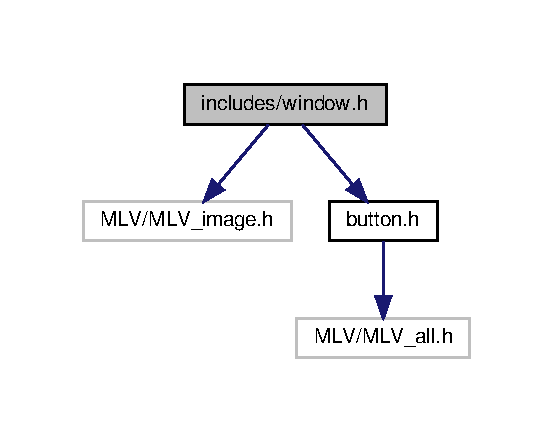
\includegraphics[width=266pt]{window_8h__incl}
\end{center}
\end{figure}
This graph shows which files directly or indirectly include this file\+:
\nopagebreak
\begin{figure}[H]
\begin{center}
\leavevmode
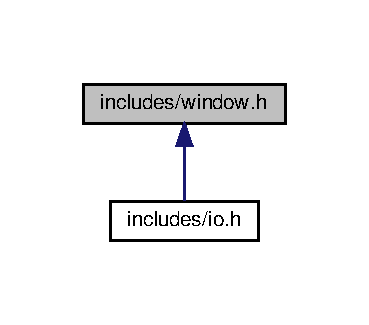
\includegraphics[width=177pt]{window_8h__dep__incl}
\end{center}
\end{figure}
\subsection*{Data Structures}
\begin{DoxyCompactItemize}
\item 
struct \hyperlink{structWin}{Win}
\end{DoxyCompactItemize}
\subsection*{Macros}
\begin{DoxyCompactItemize}
\item 
\#define \hyperlink{window_8h_a07c883b063ae8a373a3c9b5356f5fa8d}{S\+I\+Z\+E\+\_\+\+I\+M\+A\+GE}~512
\item 
\#define \hyperlink{window_8h_a697478ff051a58c25679decfec6480af}{B\+C\+K\+\_\+\+G\+R\+O\+U\+N\+D\+\_\+\+C\+O\+L\+OR}~= M\+L\+V\+\_\+\+C\+O\+L\+O\+R\+\_\+\+B\+L\+A\+CK
\end{DoxyCompactItemize}
\subsection*{Functions}
\begin{DoxyCompactItemize}
\item 
void \hyperlink{window_8h_aff2959875cb29ac85a62acd8c751074b}{init\+\_\+window\+\_\+informations} (\hyperlink{structWin}{Win} $\ast$info)
\begin{DoxyCompactList}\small\item\em This function initialise all variales needed for future handling of window informations. \end{DoxyCompactList}\item 
int \hyperlink{window_8h_a58d67052c9050874b7e97f30e67fa4d5}{place\+\_\+element\+\_\+in\+\_\+window} (\hyperlink{structWin}{Win} $\ast$info)
\begin{DoxyCompactList}\small\item\em This function places all buttons in the window and intialises them their base apearence. \end{DoxyCompactList}\item 
void \hyperlink{window_8h_a189a1e112375436240698f1744e47058}{display\+\_\+base\+\_\+window} (\hyperlink{structWin}{Win} $\ast$info)
\begin{DoxyCompactList}\small\item\em This function displays all elements in the window. \end{DoxyCompactList}\item 
int \hyperlink{window_8h_ae450a64f34975275e0ac426f0b38b97e}{update\+\_\+event} (\hyperlink{structWin}{Win} $\ast$info, \hyperlink{structMouse}{Mouse} $\ast$mouse)
\begin{DoxyCompactList}\small\item\em This function goes throught the liste of recent events and updated the window buttons accordingly using \textquotesingle{}button\+\_\+update\textquotesingle{} (button.\+c). \end{DoxyCompactList}\end{DoxyCompactItemize}


\subsection{Macro Definition Documentation}
\mbox{\Hypertarget{window_8h_a697478ff051a58c25679decfec6480af}\label{window_8h_a697478ff051a58c25679decfec6480af}} 
\index{window.\+h@{window.\+h}!B\+C\+K\+\_\+\+G\+R\+O\+U\+N\+D\+\_\+\+C\+O\+L\+OR@{B\+C\+K\+\_\+\+G\+R\+O\+U\+N\+D\+\_\+\+C\+O\+L\+OR}}
\index{B\+C\+K\+\_\+\+G\+R\+O\+U\+N\+D\+\_\+\+C\+O\+L\+OR@{B\+C\+K\+\_\+\+G\+R\+O\+U\+N\+D\+\_\+\+C\+O\+L\+OR}!window.\+h@{window.\+h}}
\subsubsection{\texorpdfstring{B\+C\+K\+\_\+\+G\+R\+O\+U\+N\+D\+\_\+\+C\+O\+L\+OR}{BCK\_GROUND\_COLOR}}
{\footnotesize\ttfamily \#define B\+C\+K\+\_\+\+G\+R\+O\+U\+N\+D\+\_\+\+C\+O\+L\+OR~= M\+L\+V\+\_\+\+C\+O\+L\+O\+R\+\_\+\+B\+L\+A\+CK}

\mbox{\Hypertarget{window_8h_a07c883b063ae8a373a3c9b5356f5fa8d}\label{window_8h_a07c883b063ae8a373a3c9b5356f5fa8d}} 
\index{window.\+h@{window.\+h}!S\+I\+Z\+E\+\_\+\+I\+M\+A\+GE@{S\+I\+Z\+E\+\_\+\+I\+M\+A\+GE}}
\index{S\+I\+Z\+E\+\_\+\+I\+M\+A\+GE@{S\+I\+Z\+E\+\_\+\+I\+M\+A\+GE}!window.\+h@{window.\+h}}
\subsubsection{\texorpdfstring{S\+I\+Z\+E\+\_\+\+I\+M\+A\+GE}{SIZE\_IMAGE}}
{\footnotesize\ttfamily \#define S\+I\+Z\+E\+\_\+\+I\+M\+A\+GE~512}



\subsection{Function Documentation}
\mbox{\Hypertarget{window_8h_a189a1e112375436240698f1744e47058}\label{window_8h_a189a1e112375436240698f1744e47058}} 
\index{window.\+h@{window.\+h}!display\+\_\+base\+\_\+window@{display\+\_\+base\+\_\+window}}
\index{display\+\_\+base\+\_\+window@{display\+\_\+base\+\_\+window}!window.\+h@{window.\+h}}
\subsubsection{\texorpdfstring{display\+\_\+base\+\_\+window()}{display\_base\_window()}}
{\footnotesize\ttfamily void display\+\_\+base\+\_\+window (\begin{DoxyParamCaption}\item[{\hyperlink{structWin}{Win} $\ast$}]{info }\end{DoxyParamCaption})}



This function displays all elements in the window. 


\begin{DoxyParams}{Parameters}
{\em info} & a pointer on the structure holding all window-\/relevent infromation. \\
\hline
\end{DoxyParams}
\begin{DoxyReturn}{Returns}
Nothing. 
\end{DoxyReturn}
\mbox{\Hypertarget{window_8h_aff2959875cb29ac85a62acd8c751074b}\label{window_8h_aff2959875cb29ac85a62acd8c751074b}} 
\index{window.\+h@{window.\+h}!init\+\_\+window\+\_\+informations@{init\+\_\+window\+\_\+informations}}
\index{init\+\_\+window\+\_\+informations@{init\+\_\+window\+\_\+informations}!window.\+h@{window.\+h}}
\subsubsection{\texorpdfstring{init\+\_\+window\+\_\+informations()}{init\_window\_informations()}}
{\footnotesize\ttfamily void init\+\_\+window\+\_\+informations (\begin{DoxyParamCaption}\item[{\hyperlink{structWin}{Win} $\ast$}]{info }\end{DoxyParamCaption})}



This function initialise all variales needed for future handling of window informations. 


\begin{DoxyParams}{Parameters}
{\em info} & a pointer on the structue holding all the information. \\
\hline
\end{DoxyParams}
\begin{DoxyReturn}{Returns}
Nothing. 
\end{DoxyReturn}
\mbox{\Hypertarget{window_8h_a58d67052c9050874b7e97f30e67fa4d5}\label{window_8h_a58d67052c9050874b7e97f30e67fa4d5}} 
\index{window.\+h@{window.\+h}!place\+\_\+element\+\_\+in\+\_\+window@{place\+\_\+element\+\_\+in\+\_\+window}}
\index{place\+\_\+element\+\_\+in\+\_\+window@{place\+\_\+element\+\_\+in\+\_\+window}!window.\+h@{window.\+h}}
\subsubsection{\texorpdfstring{place\+\_\+element\+\_\+in\+\_\+window()}{place\_element\_in\_window()}}
{\footnotesize\ttfamily int place\+\_\+element\+\_\+in\+\_\+window (\begin{DoxyParamCaption}\item[{\hyperlink{structWin}{Win} $\ast$}]{info }\end{DoxyParamCaption})}



This function places all buttons in the window and intialises them their base apearence. 

It allocates memory on the \textquotesingle{}button\+\_\+array\textquotesingle{} field and updates \textquotesingle{}nb\+\_\+button\textquotesingle{} accordingly. 
\begin{DoxyParams}{Parameters}
{\em info} & a pointer on the structure holding all window information. \\
\hline
\end{DoxyParams}
\begin{DoxyReturn}{Returns}
0\+: Memory allocation error. 1\+: All good. 
\end{DoxyReturn}
\mbox{\Hypertarget{window_8h_ae450a64f34975275e0ac426f0b38b97e}\label{window_8h_ae450a64f34975275e0ac426f0b38b97e}} 
\index{window.\+h@{window.\+h}!update\+\_\+event@{update\+\_\+event}}
\index{update\+\_\+event@{update\+\_\+event}!window.\+h@{window.\+h}}
\subsubsection{\texorpdfstring{update\+\_\+event()}{update\_event()}}
{\footnotesize\ttfamily int update\+\_\+event (\begin{DoxyParamCaption}\item[{\hyperlink{structWin}{Win} $\ast$}]{info,  }\item[{\hyperlink{structMouse}{Mouse} $\ast$}]{mouse }\end{DoxyParamCaption})}



This function goes throught the liste of recent events and updated the window buttons accordingly using \textquotesingle{}button\+\_\+update\textquotesingle{} (button.\+c). 


\begin{DoxyParams}{Parameters}
{\em info} & a pointer on the structure holding all window information. \\
\hline
{\em mouse} & -\/$>$ a pointer on a structure to store all mouse relvent informations. \\
\hline
\end{DoxyParams}
\begin{DoxyReturn}{Returns}
info.\+nb\+\_\+button -\/$>$ no event affecting the window buttons found. \mbox{[}0; nb\+\_\+button\mbox{[} -\/$>$ the numbre in the button\+\_\+array field of info corresponding to the affected button. 
\end{DoxyReturn}

\hypertarget{zone_8h}{}\section{includes/zone.h File Reference}
\label{zone_8h}\index{includes/zone.\+h@{includes/zone.\+h}}
This graph shows which files directly or indirectly include this file\+:
\nopagebreak
\begin{figure}[H]
\begin{center}
\leavevmode
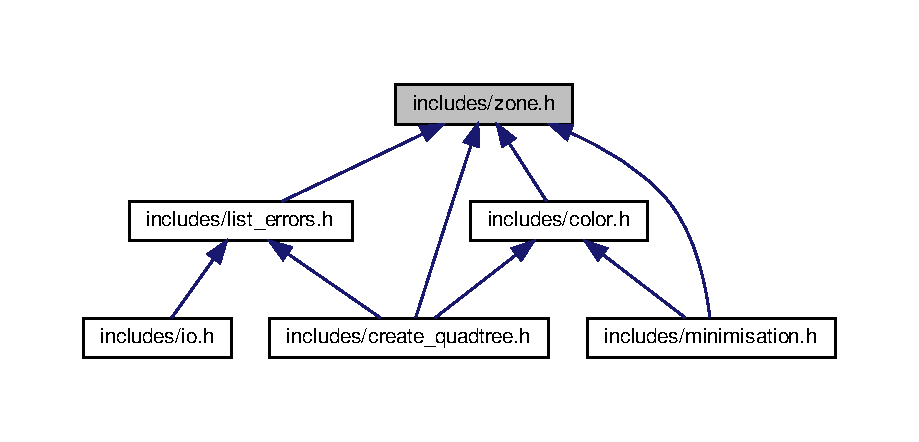
\includegraphics[width=350pt]{zone_8h__dep__incl}
\end{center}
\end{figure}
\subsection*{Data Structures}
\begin{DoxyCompactItemize}
\item 
struct \hyperlink{structZone}{Zone}
\end{DoxyCompactItemize}
\subsection*{Functions}
\begin{DoxyCompactItemize}
\item 
\hyperlink{structZone}{Zone} \hyperlink{zone_8h_a880e5e8bcb5437e630a29139047f9de7}{return\+\_\+zone} (int x1, int y1, int x2, int y2)
\begin{DoxyCompactList}\small\item\em Return a struct \char`\"{}\+Zone\char`\"{} with the fields equal to those in parameters. \end{DoxyCompactList}\item 
\hyperlink{structZone}{Zone} \hyperlink{zone_8h_a5de6549b4a1b43944a855c3ebef65626}{no\+\_\+zone} (\hyperlink{structZone}{Zone} zone)
\begin{DoxyCompactList}\small\item\em Return the NO zone of the \char`\"{}zone\char`\"{} in parameter. \end{DoxyCompactList}\item 
\hyperlink{structZone}{Zone} \hyperlink{zone_8h_a4fb27715d3e5161f19f6a58349db8327}{ne\+\_\+zone} (\hyperlink{structZone}{Zone} zone)
\begin{DoxyCompactList}\small\item\em Return the NE zone of the \char`\"{}zone\char`\"{} in parameter. \end{DoxyCompactList}\item 
\hyperlink{structZone}{Zone} \hyperlink{zone_8h_a35c35ccd584138ee8f7d6d6cb39f9ea6}{so\+\_\+zone} (\hyperlink{structZone}{Zone} zone)
\begin{DoxyCompactList}\small\item\em Return the SO zone of the \char`\"{}zone\char`\"{} in parameter. \end{DoxyCompactList}\item 
\hyperlink{structZone}{Zone} \hyperlink{zone_8h_aa8f0ac5486b44c421cd41e66ef06abab}{se\+\_\+zone} (\hyperlink{structZone}{Zone} zone)
\begin{DoxyCompactList}\small\item\em Return the SE zone of the \char`\"{}zone\char`\"{} in parameter. \end{DoxyCompactList}\end{DoxyCompactItemize}


\subsection{Function Documentation}
\mbox{\Hypertarget{zone_8h_a4fb27715d3e5161f19f6a58349db8327}\label{zone_8h_a4fb27715d3e5161f19f6a58349db8327}} 
\index{zone.\+h@{zone.\+h}!ne\+\_\+zone@{ne\+\_\+zone}}
\index{ne\+\_\+zone@{ne\+\_\+zone}!zone.\+h@{zone.\+h}}
\subsubsection{\texorpdfstring{ne\+\_\+zone()}{ne\_zone()}}
{\footnotesize\ttfamily \hyperlink{structZone}{Zone} ne\+\_\+zone (\begin{DoxyParamCaption}\item[{\hyperlink{structZone}{Zone}}]{zone }\end{DoxyParamCaption})}



Return the NE zone of the \char`\"{}zone\char`\"{} in parameter. 


\begin{DoxyParams}{Parameters}
{\em zone} & The zone we\textquotesingle{}ll subdivise to get its NE zone \\
\hline
\end{DoxyParams}
\begin{DoxyReturn}{Returns}
The NE zone of parameter \char`\"{}zone\char`\"{} 
\end{DoxyReturn}
\mbox{\Hypertarget{zone_8h_a5de6549b4a1b43944a855c3ebef65626}\label{zone_8h_a5de6549b4a1b43944a855c3ebef65626}} 
\index{zone.\+h@{zone.\+h}!no\+\_\+zone@{no\+\_\+zone}}
\index{no\+\_\+zone@{no\+\_\+zone}!zone.\+h@{zone.\+h}}
\subsubsection{\texorpdfstring{no\+\_\+zone()}{no\_zone()}}
{\footnotesize\ttfamily \hyperlink{structZone}{Zone} no\+\_\+zone (\begin{DoxyParamCaption}\item[{\hyperlink{structZone}{Zone}}]{zone }\end{DoxyParamCaption})}



Return the NO zone of the \char`\"{}zone\char`\"{} in parameter. 


\begin{DoxyParams}{Parameters}
{\em zone} & The zone we\textquotesingle{}ll subdivise to get its NO zone \\
\hline
\end{DoxyParams}
\begin{DoxyReturn}{Returns}
The NO zone of parameter \char`\"{}zone\char`\"{} 
\end{DoxyReturn}
\mbox{\Hypertarget{zone_8h_a880e5e8bcb5437e630a29139047f9de7}\label{zone_8h_a880e5e8bcb5437e630a29139047f9de7}} 
\index{zone.\+h@{zone.\+h}!return\+\_\+zone@{return\+\_\+zone}}
\index{return\+\_\+zone@{return\+\_\+zone}!zone.\+h@{zone.\+h}}
\subsubsection{\texorpdfstring{return\+\_\+zone()}{return\_zone()}}
{\footnotesize\ttfamily \hyperlink{structZone}{Zone} return\+\_\+zone (\begin{DoxyParamCaption}\item[{int}]{x1,  }\item[{int}]{y1,  }\item[{int}]{x2,  }\item[{int}]{y2 }\end{DoxyParamCaption})}



Return a struct \char`\"{}\+Zone\char`\"{} with the fields equal to those in parameters. 


\begin{DoxyParams}{Parameters}
{\em x1} & Field x1 of the zone we are returning \\
\hline
{\em y1} & Field y1 of the zone we are returning \\
\hline
{\em x2} & Field x2 of the zone we are returning \\
\hline
{\em y2} & Field y2 of the zone we are returning \\
\hline
\end{DoxyParams}
\begin{DoxyReturn}{Returns}
\hyperlink{structZone}{Zone} with x1, y1, x2, y2 parameters values 
\end{DoxyReturn}
\mbox{\Hypertarget{zone_8h_aa8f0ac5486b44c421cd41e66ef06abab}\label{zone_8h_aa8f0ac5486b44c421cd41e66ef06abab}} 
\index{zone.\+h@{zone.\+h}!se\+\_\+zone@{se\+\_\+zone}}
\index{se\+\_\+zone@{se\+\_\+zone}!zone.\+h@{zone.\+h}}
\subsubsection{\texorpdfstring{se\+\_\+zone()}{se\_zone()}}
{\footnotesize\ttfamily \hyperlink{structZone}{Zone} se\+\_\+zone (\begin{DoxyParamCaption}\item[{\hyperlink{structZone}{Zone}}]{zone }\end{DoxyParamCaption})}



Return the SE zone of the \char`\"{}zone\char`\"{} in parameter. 


\begin{DoxyParams}{Parameters}
{\em zone} & The zone we\textquotesingle{}ll subdivise to get its SE zone \\
\hline
\end{DoxyParams}
\begin{DoxyReturn}{Returns}
The SE zone of parameter \char`\"{}zone\char`\"{} 
\end{DoxyReturn}
\mbox{\Hypertarget{zone_8h_a35c35ccd584138ee8f7d6d6cb39f9ea6}\label{zone_8h_a35c35ccd584138ee8f7d6d6cb39f9ea6}} 
\index{zone.\+h@{zone.\+h}!so\+\_\+zone@{so\+\_\+zone}}
\index{so\+\_\+zone@{so\+\_\+zone}!zone.\+h@{zone.\+h}}
\subsubsection{\texorpdfstring{so\+\_\+zone()}{so\_zone()}}
{\footnotesize\ttfamily \hyperlink{structZone}{Zone} so\+\_\+zone (\begin{DoxyParamCaption}\item[{\hyperlink{structZone}{Zone}}]{zone }\end{DoxyParamCaption})}



Return the SO zone of the \char`\"{}zone\char`\"{} in parameter. 


\begin{DoxyParams}{Parameters}
{\em zone} & The zone we\textquotesingle{}ll subdivise to get its SO zone \\
\hline
\end{DoxyParams}
\begin{DoxyReturn}{Returns}
The SO zone of parameter \char`\"{}zone\char`\"{} 
\end{DoxyReturn}

%--- End generated contents ---

% Index
\backmatter
\newpage
\phantomsection
\clearemptydoublepage
\addcontentsline{toc}{chapter}{Index}
\printindex

\end{document}
